\section[Le Memorie]{Le Memorie}
\label{sec:memory}
\sectionframe{images/covers/cover_sd_memory.png}{Le Memorie}	 


\subsection[Lo scopo delle memorie]{Lo scopo delle memorie}
\begin{frame}
	\frametitle{Lo scopo delle memorie}
	
	\begin{block}{Lo scopo delle memorie}
		La memoria, in informatica, è un elemento di un computer che ha il compito di garantire la \textbf{persistenza dei dati e/o delle istruzioni dei programmi}.\\\vspace{0.5em}
		Esistono diversi \textbf{tipi di memoria} e la loro realizzazione fisica dà vita a vari supporti di memorizzazione differenti tra loro.\\\vspace{0.5em}
		Noi ne approfondiremo alcune:
		
		\begin{itemize}
			\item I flip-flop
			\item La ROM
			\item La RAM
			\item La memoria di massa
		\end{itemize}
		
	\end{block}
	
\end{frame}


\subsection[La memorie volatili e non volatili]{La memorie volatili e non volatili}
\begin{frame}
	\frametitle{La memorie volatili e non volatili}
	 
	\begin{block}{La memoria volatile}
		è una memoria che \textbf{necessita dell'alimentazione elettrica} continua al fine di \textbf{mantenere memorizzate le informazioni}. Questo tipo di memorie sono anche note come memorie temporanee.
	\end{block}
	\vspace{1.0em}
	\begin{block}{La memoria non volatile}
		è una tipologia di memoria in grado di \textbf{mantenere le informazioni anche quando non viene alimentata}.
	\end{block}
	
\end{frame}


\subsection[Il collo di bottiglia delle memorie]{Il collo di bottiglia delle memorie}
\begin{frame}
	\frametitle{Il collo di bottiglia delle memorie}
	 
	\begin{block}{Il collo di bottiglia}
		Il \textbf{collo di bottiglia} è un fenomeno che si verifica quando le prestazioni di un sistema o le sue capacità sono fortemente vincolate da un singolo componente. Il termine è una metafora del collo di bottiglia reale, che limita il flusso d'uscita dell'acqua.
	\end{block}
	\pause
	\begin{block}{Le prestazioni della memoria RAM}
		Le velocità delle CPU si sono evolute nel tempo aumentando ad un ritmo esponenziale (vedi \hyperlink{subsub:moore_law}{\textbf{Legge di Moore}}).\\
		
		Il canale di comunicazione tra \textbf{CPU} e \textbf{memoria} è diventato quindi \textbf{punto critico} del sistema in quanto l'evoluzione delle velocità di accesso alle memorie non è riuscita a tenere il passo con il ritmo di miglioramento di prestazioni delle CPU (collo di bottiglia).\\
		Determinante è stato anche il fattore costo dei componenti elettronici.
	\end{block}
	
\end{frame}


\subsubsection[Il fattore costo]{Il fattore costo}
\begin{frame}
	\frametitle{Il fattore costo}
	
	\begin{block}{Il fattore costo}
		I \textbf{registri} di memoria della CPU sono in assoluto le \textbf{memorie più veloci} che abbiamo a disposizione. Non possiamo aggiungere infiniti registri a un chip. Occupano spazio e se espandiamo il chip per aggiungere più registri, diventa troppo costoso.\\\vspace{0.8em}
		
		Tuttavia la \textbf{RAM} è molto \textbf{più lenta della CPU}, per migliorare le prestazioni vengono quindi combinati tipi di memoria veloce con tipi di memoria più capienti e meno costose (a parità di capacità) se pur più lente (cache).
	\end{block}
	
\end{frame}


\subsubsection[L'organizzazione in livelli gerarchici]{L'organizzazione in livelli gerarchici}
\begin{frame}
	\frametitle{L'organizzazione in livelli gerarchici}
	 
	\begin{block}{La gerarchia delle memorie}
		La memoria del PC viene quindi organizzata in \textbf{livelli gerarchici}, ogni livello è caratterizzato da una \underline{\textbf{dimensione crescente}} e da un \underline{\textbf{tempo di accesso decrescente}}: registri di memoria, cache L1, L2 (anche L3 ed L4 nei processori più moderni), la memoria RAM e la memoria di massa.
	\end{block}
	
	\begin{figure}[!htbp] 
		\centering
		%\advance\leftskip-0.25cm
		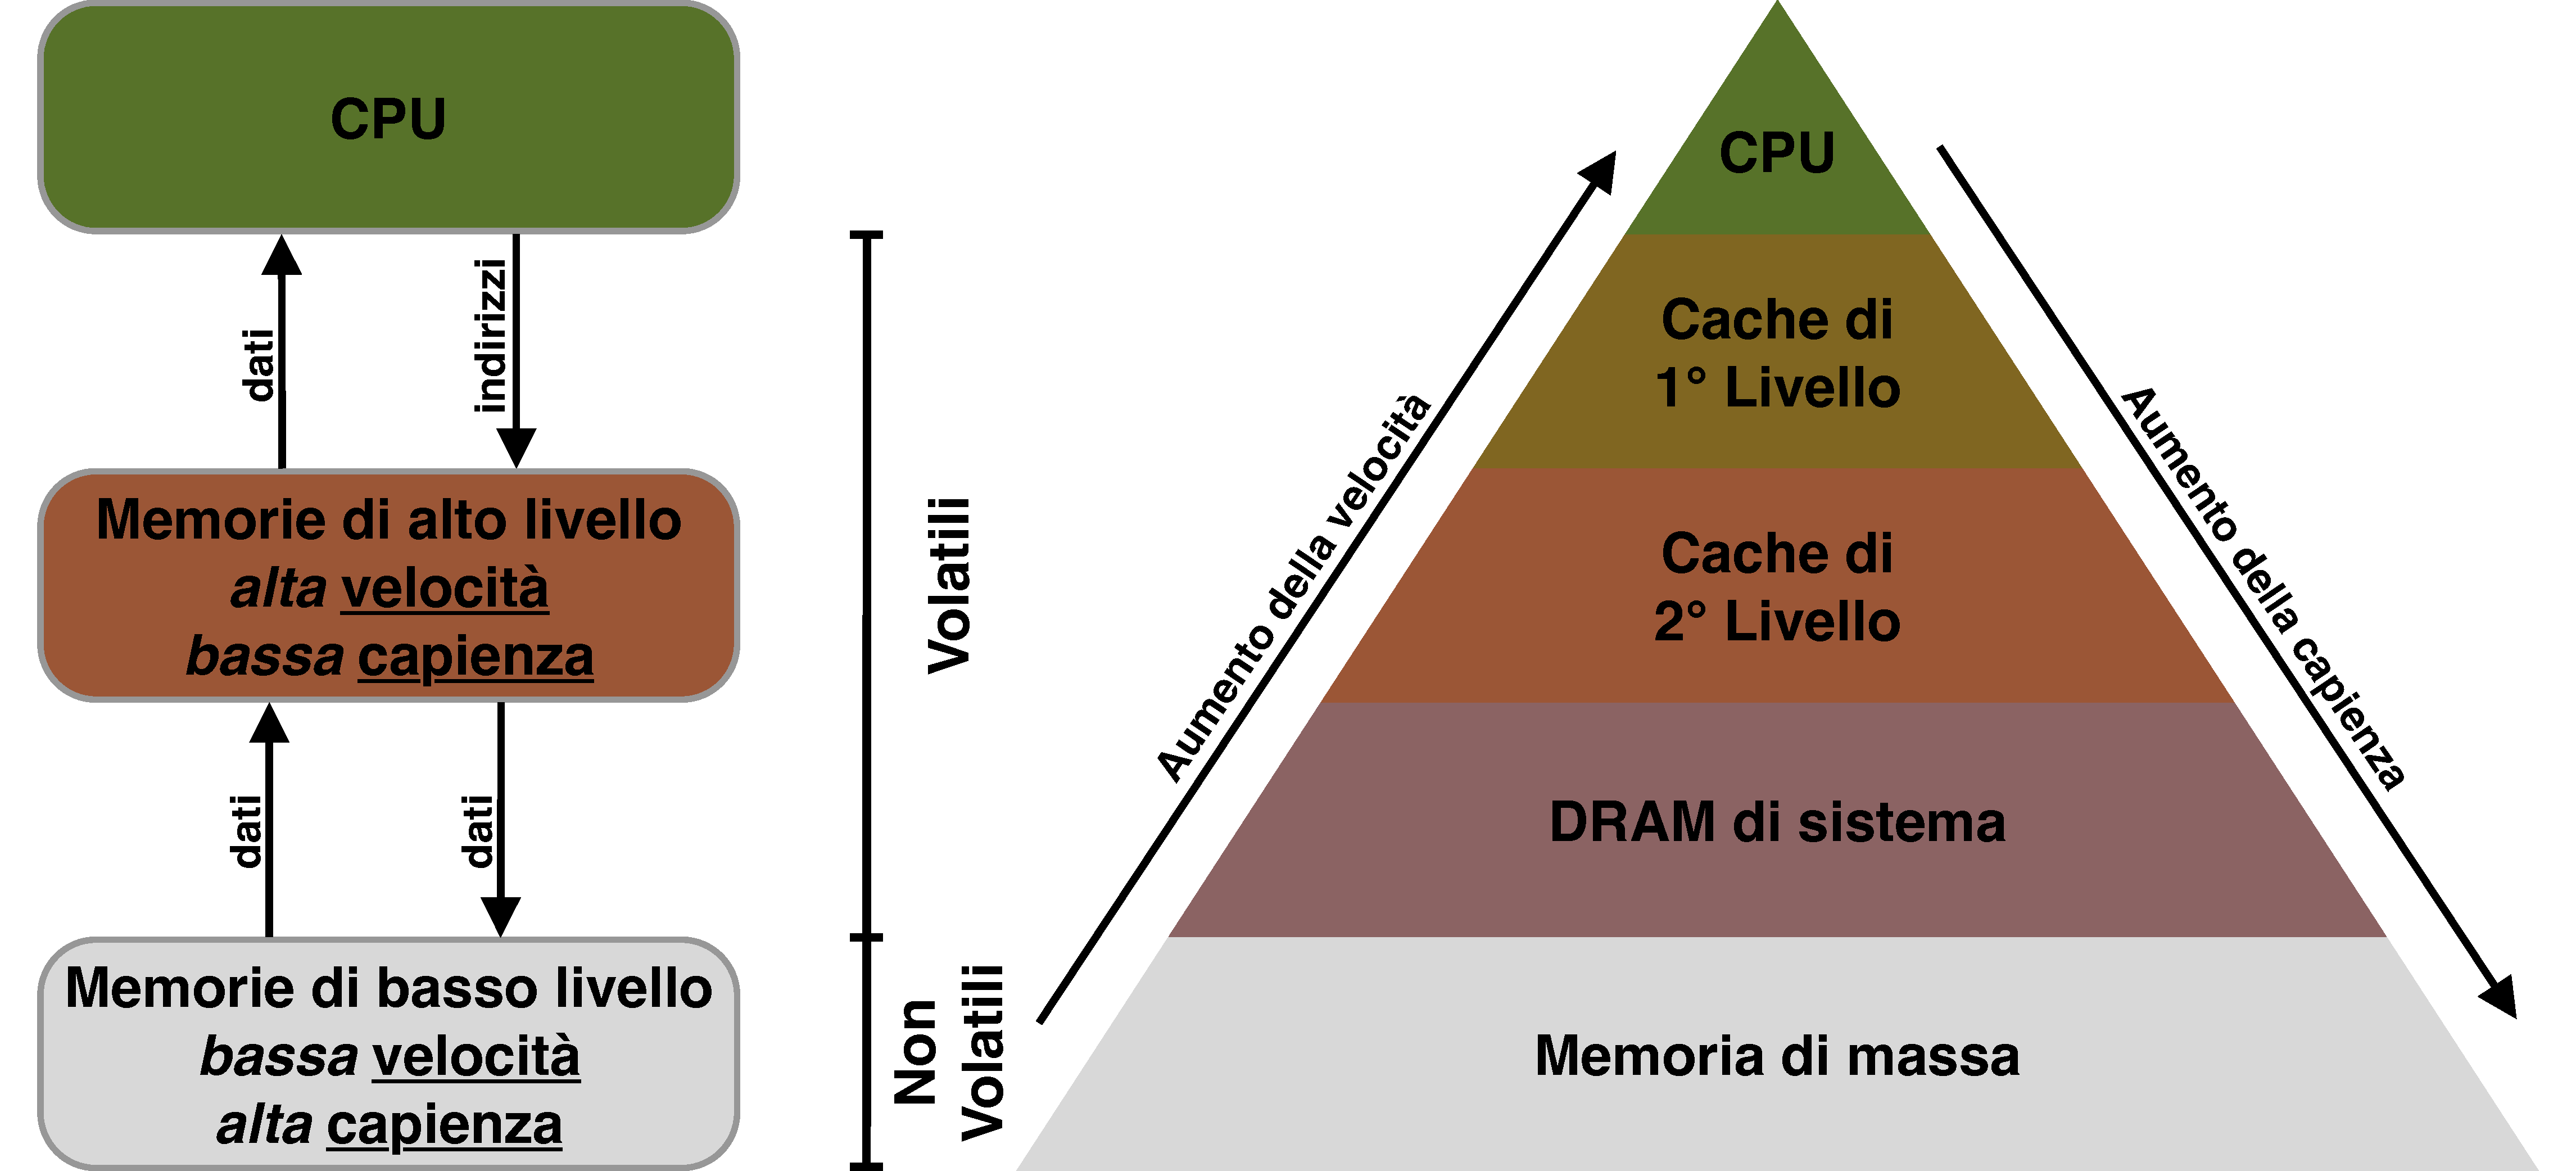
\includegraphics[width=0.8\linewidth]{images/5_memory/memory_hierarchy.pdf}
%		\caption{La CPU: CU, ALU e registri}
		\label{fig:memory_hierarchy}
	\end{figure} 

\end{frame}


\begin{frame}
	\frametitle{L'organizzazione in livelli gerarchici}

	\begin{figure}[!htbp] 
		\centering
		%\advance\leftskip-0.25cm
		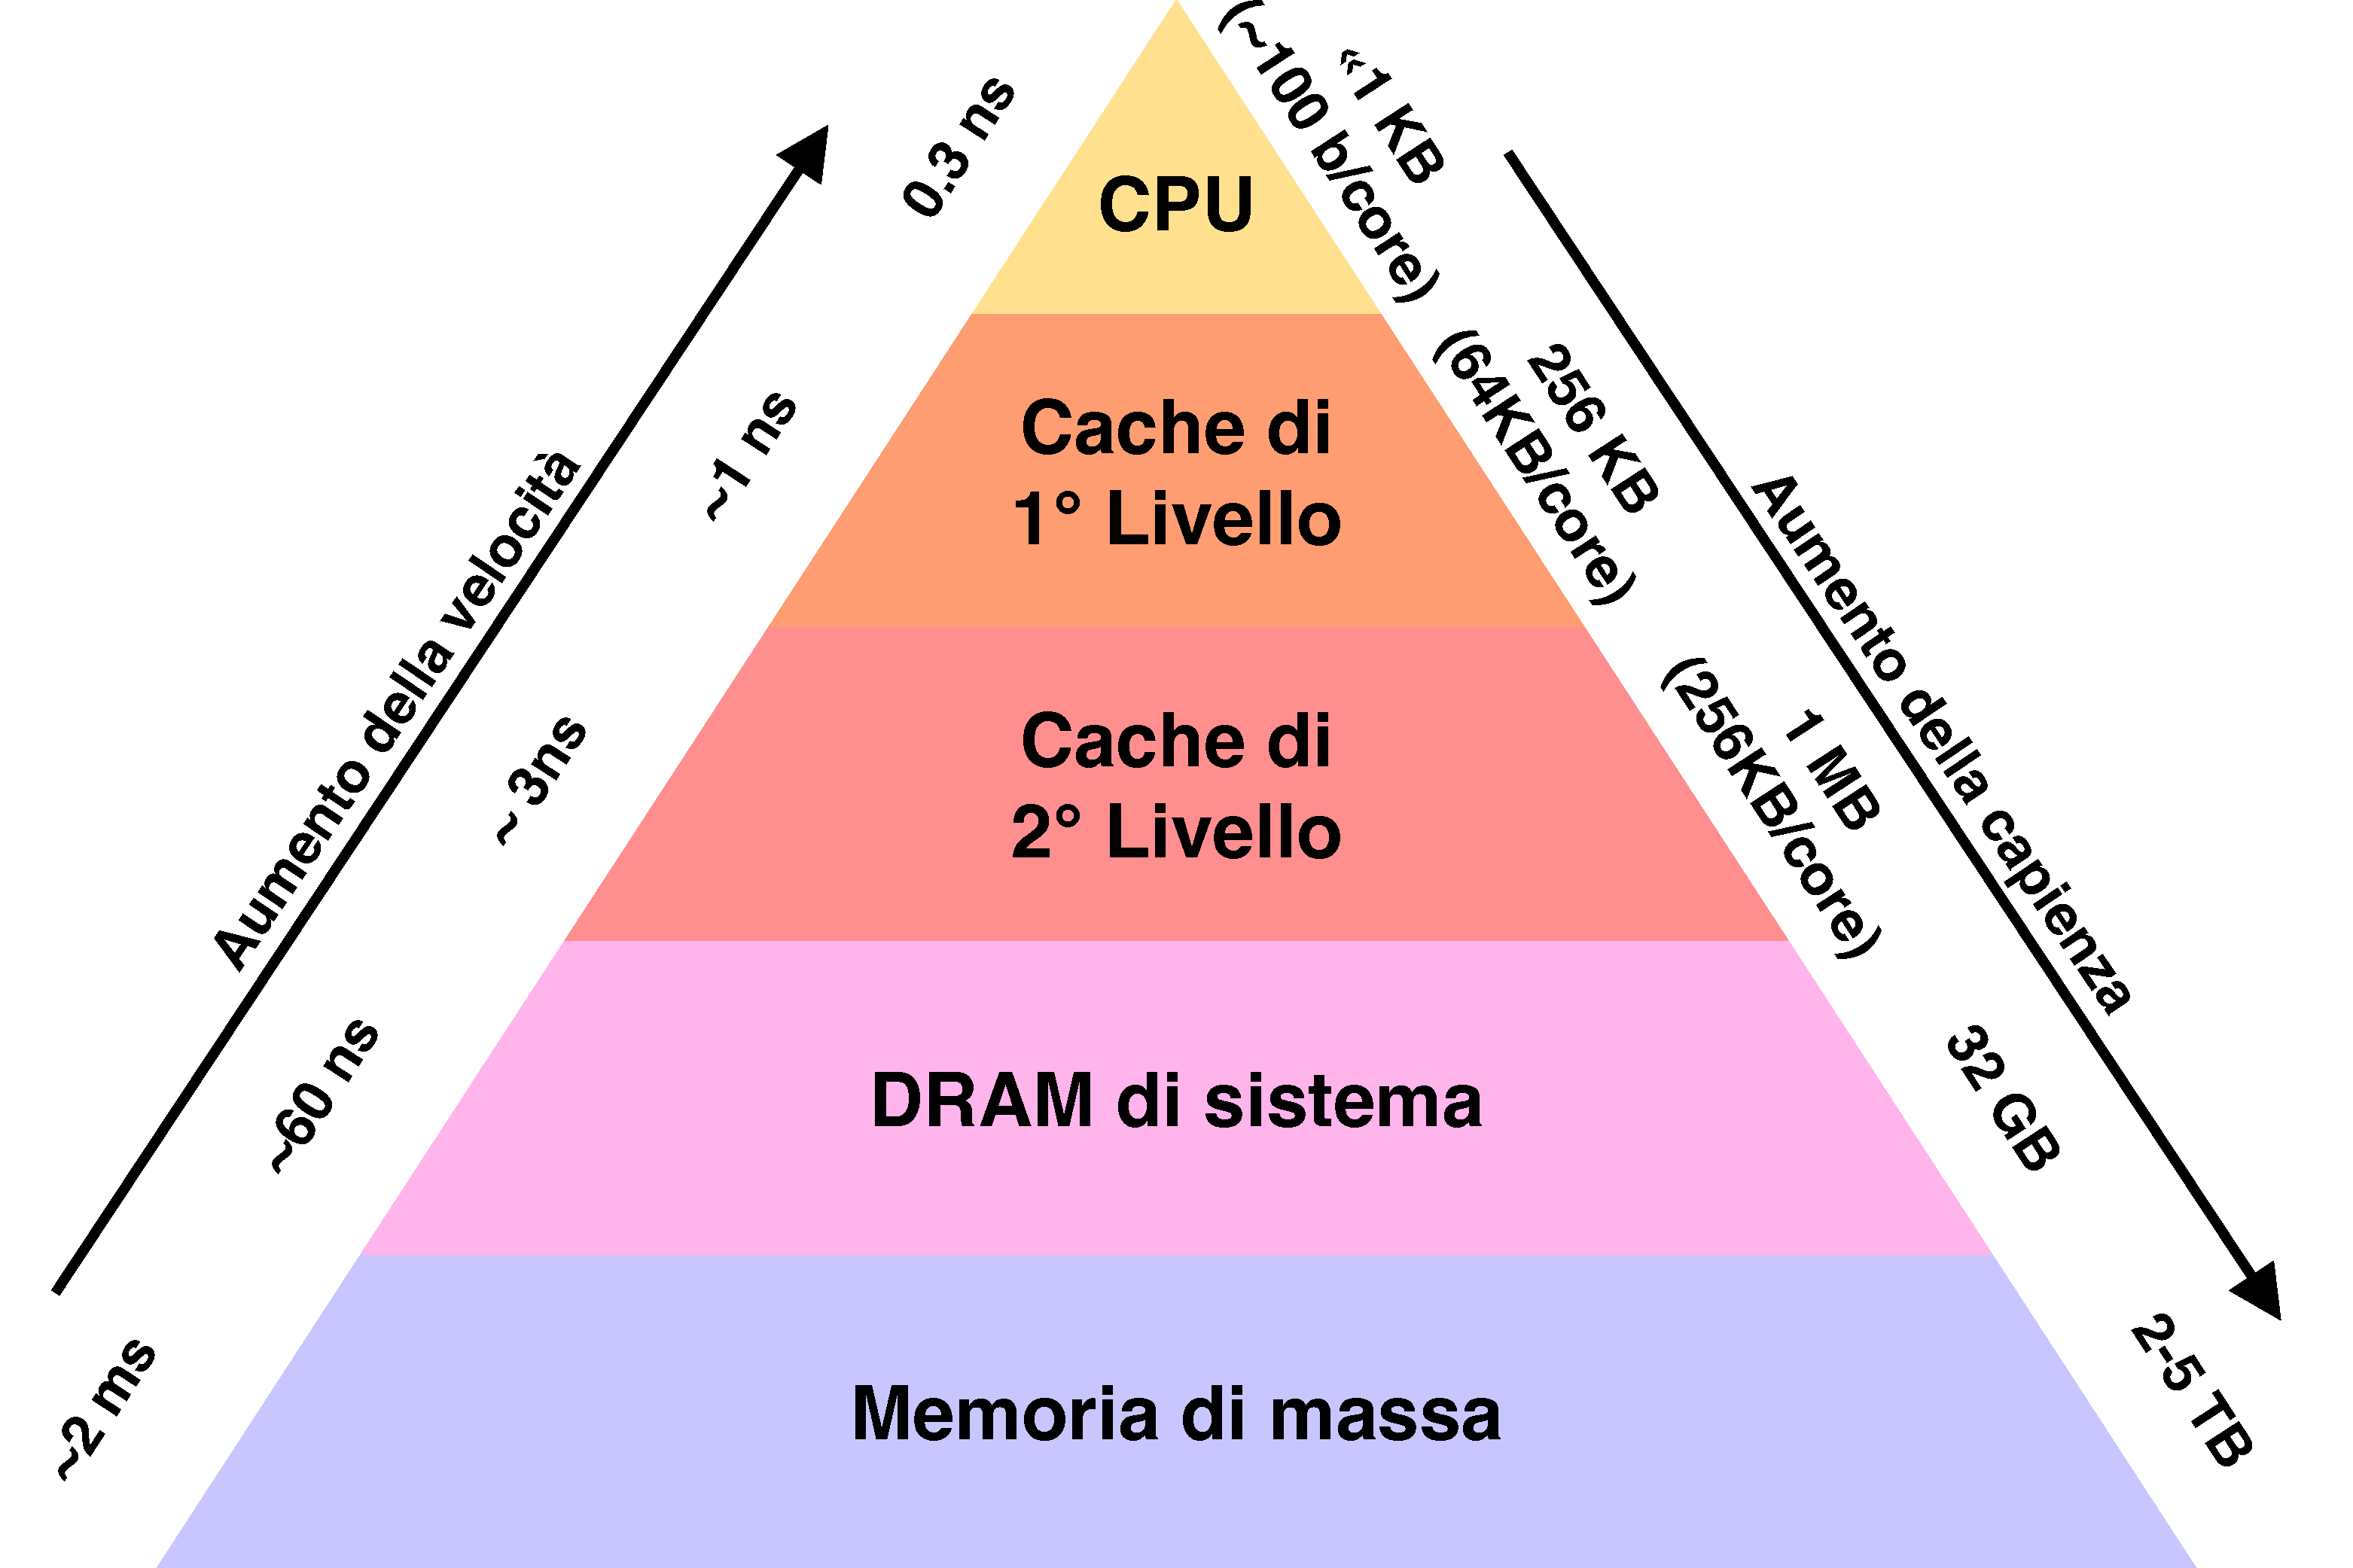
\includegraphics[width=0.9\linewidth]{images/5_memory/memory_hierarchy_info.pdf}
%		\caption{}
		\label{fig:memory_hierarchy}
	\end{figure} 

\end{frame}

\begin{frame}
	\frametitle{L'organizzazione in livelli gerarchici}
	 
	\begin{figure}[!htbp] 
		\centering
		%\advance\leftskip-0.25cm
		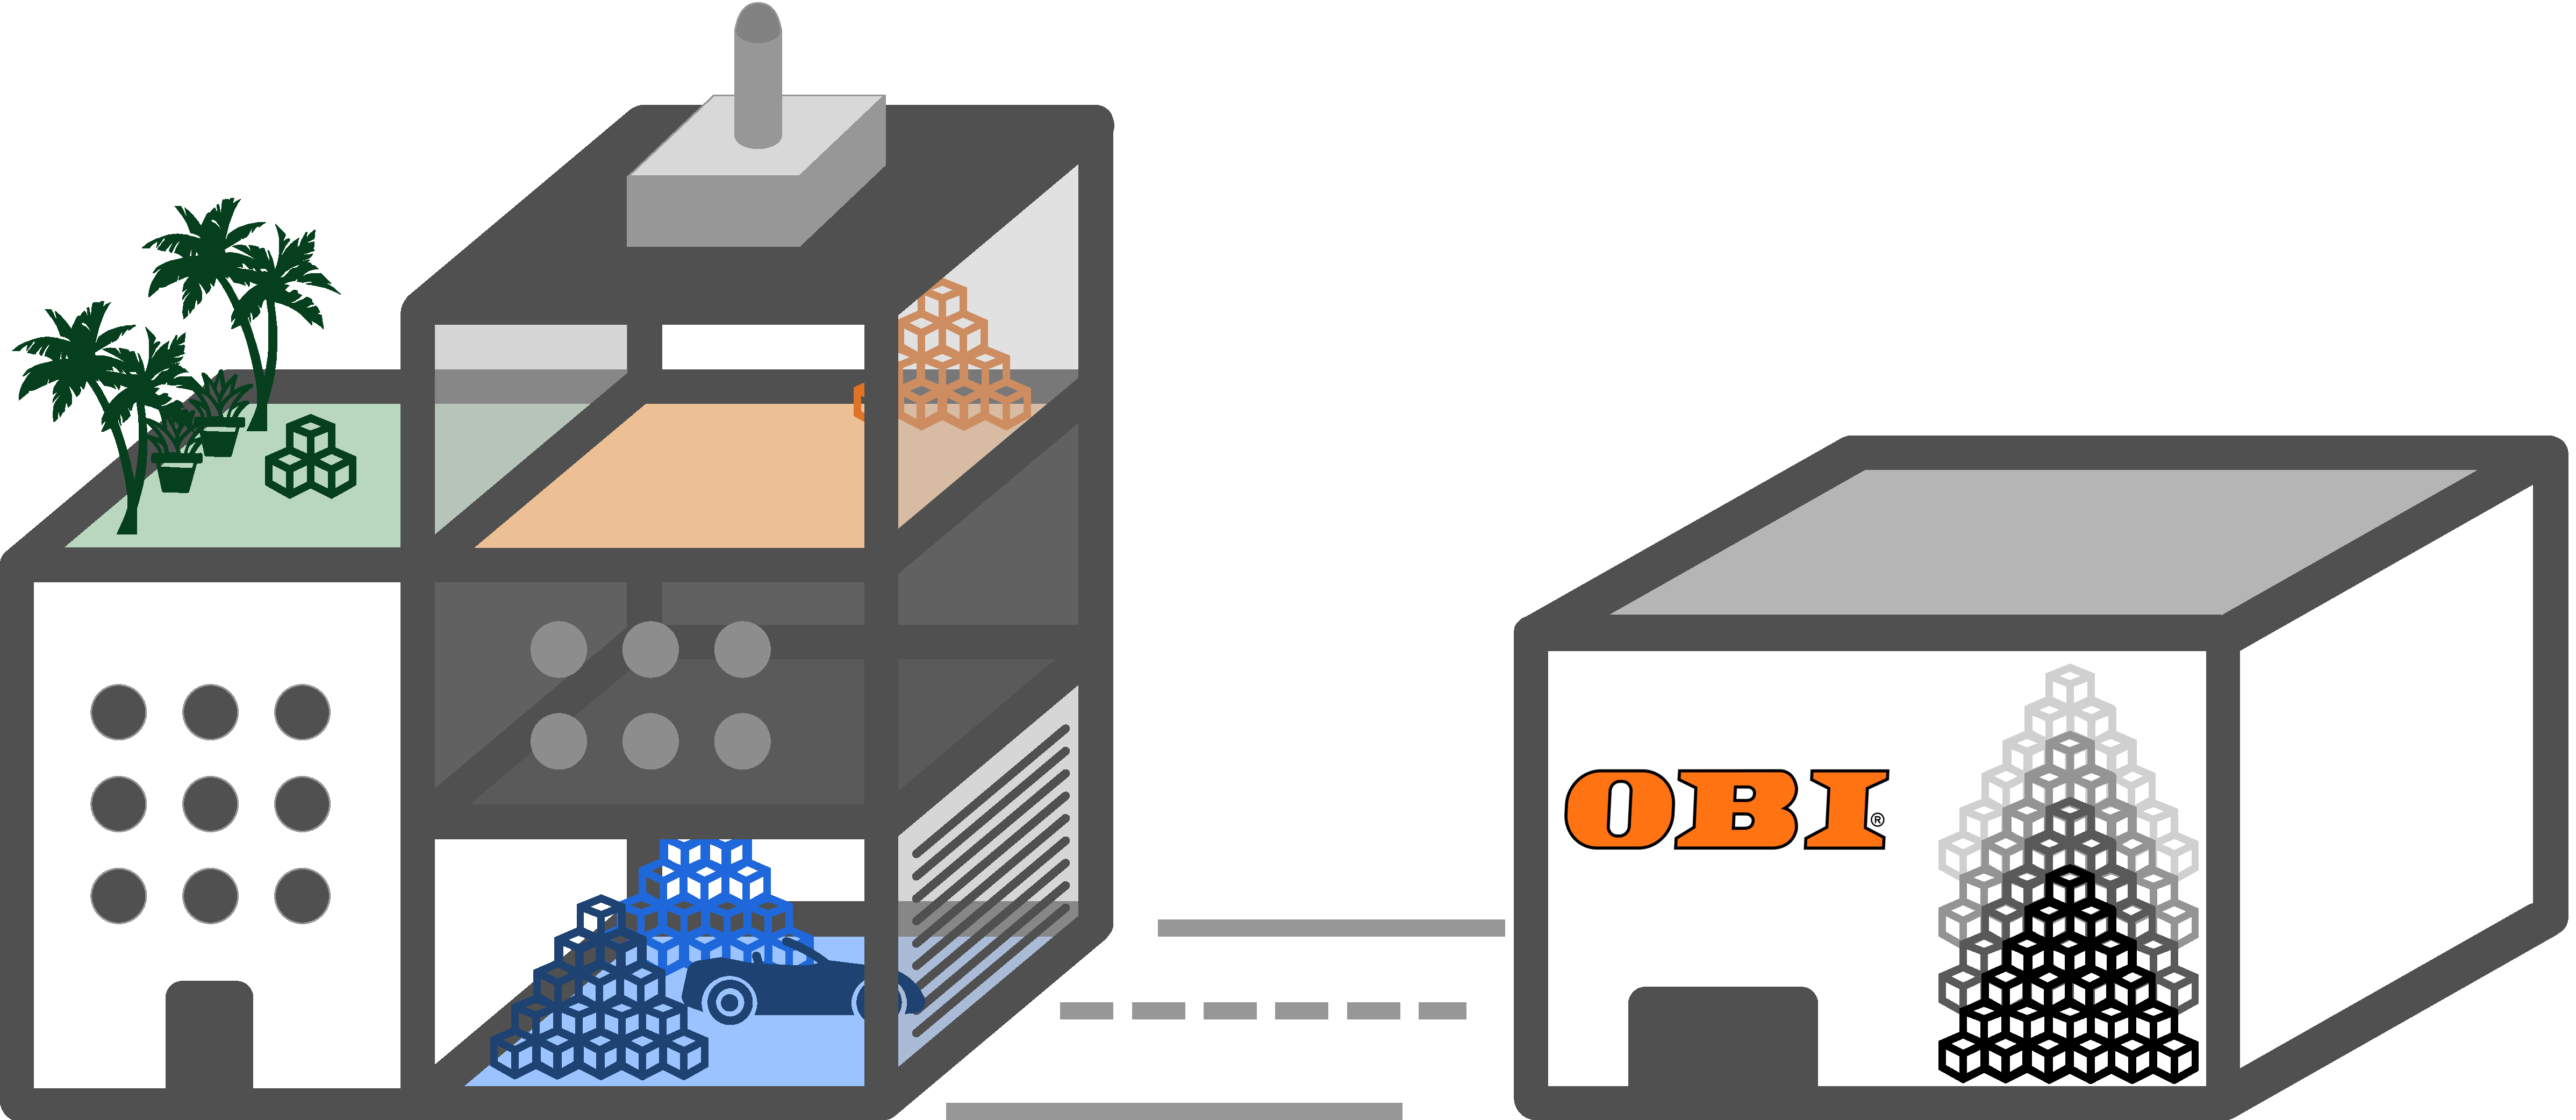
\includegraphics[width=1.0\linewidth]{images/5_memory/gardening.pdf}
		%\caption{}
	\end{figure}
	
\end{frame}

\begin{frame}
	\frametitle{L'organizzazione in livelli gerarchici}
	 
	 Immagina di vivere al terzo piano di un palazzo.\\
	 Vuoi fare giardinaggio sul tuo terrazzo, per lavorare hai bisogno di uno specifico attrezzo, ad esempio un rastrello. \pause
	 \begin{enumerate}
	 	\item se hai già un rastrello in uno dei cassetti per gli attrezzi del terrazzo (hit) procedi con i tuoi lavori, altrimenti (miss) \pause
	 	\item ti sposti in casa e cerchi il rastrello nei cassetti degli attrezzi del ripostiglio, se lo trovi (hit) torni sul terrazzo, altrimenti (miss) \pause
	 	\item ti sposti in garage e cerchi il rastrello nei cassetti degli attrezzi del garage, se lo trovi torni sul terrazzo, altrimenti (miss) \pause
	 	\item prendi la macchina e ti sposti all'OBI, cerchi il rastrello nei cassetti dell'OBI, se lo trovi torni sul terrazzo \pause
	 \end{enumerate}
	 Ogni volta che hai un hit copi questo e una piccola porzione adiacente ad essa nel livello superiore e così via fino a che non raggiungi il terrazzo. \pause
	 Ogni volta che hai un miss invece ti sposti a cercare nel livello inferiore.
	
\end{frame}


\begin{frame}
	\frametitle{L'organizzazione in livelli gerarchici}
	
	\begin{figure}[!htbp] 
		\centering
		%\advance\leftskip-0.25cm
		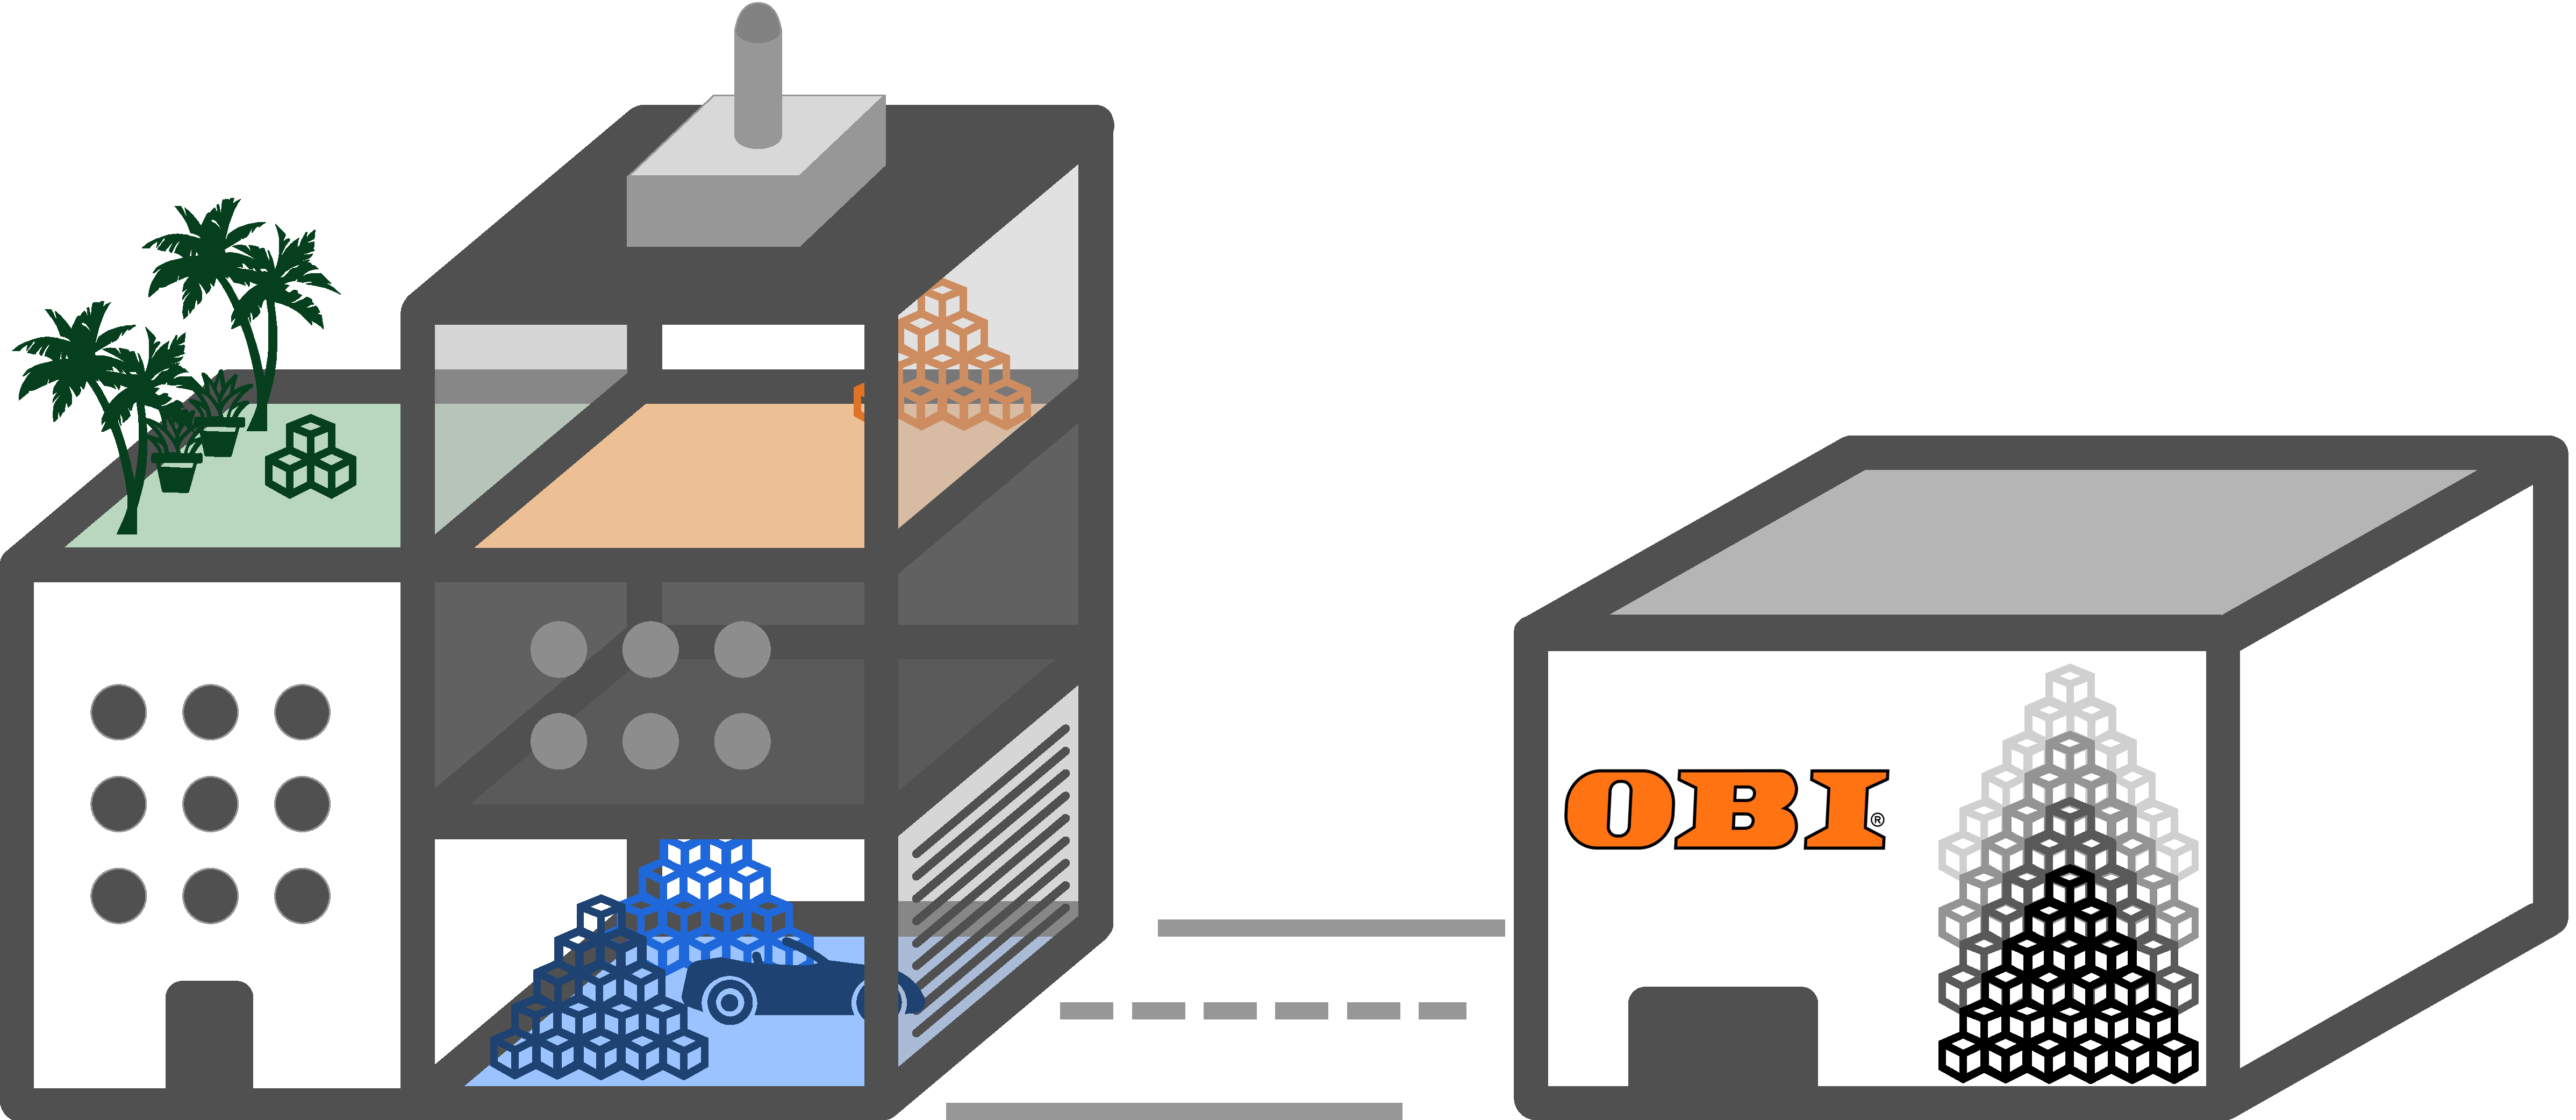
\includegraphics[width=0.6\linewidth]{images/5_memory/gardening.pdf}
		%\caption{}
	\end{figure}
	 \pause
	 Nell'esempio presentato: \pause
	 \begin{enumerate}
	 	\item il terrazzo e la abitazione: \pause \textbf{la CPU} \pause
	 	\item i cassetti degli attrezzi sul terrazzo: \pause \textbf{i registri} \pause
	 	\item i cassetti degli attrezzi nel ripostiglio: \pause la \textbf{memoria cache L1} \pause
	 	\item i cassetti degli attrezzi nel garage: \pause la \textbf{memoria cache L2} \pause
	 	\item i cassetti degli attrezzi da OBI: \pause la \textbf{RAM}
	 \end{enumerate}
	
\end{frame}


%\begin{frame}
%	\frametitle{Esercizi sulla relazione tra $\mathrm{T}$ e $f$:}
%	
%	\begin{block}{Esercizio 1: calcola il periodo $\mathrm{T}$ conoscendo la frequenza $f$}
%		Un \textbf{processore} con \textbf{frequenza di clock} (o velocità di clock) di \textbf{4.0 $\pmb{GHz}$} (giga$Hz$) esegue 4 miliardi di cicli completi al secondo.\\
%		In passato le CPU erano molto più lente di oggi e la frequenza di clock era misurata in $MHz$ (mega$Hz$) ovvero milioni di cicli completi al secondo.\\
%		\textbf{Quanto dura il periodo di clock $\pmb{\mathrm{T}}$ per il suddetto processore?}\\~\\
%		\pause
%		Ricordando che la relazione tra $\mathrm{T}$ e $f$ è del tipo $\mathrm{T} = \frac{1}{f}$ possiamo calcolare la durata del periodo di clock $\mathrm{T}$ conoscendo la frequenza $f$ come segue:\\~\\
%		\pause
%		$\quad\,\, \mathrm{T} = \frac{1}{f} = \frac{1}{4 GHz} = \frac{1}{4 \cdot 10^9 Hz} = \frac{1}{4 \cdot 10^9 1/s} = \frac{1}{4 \cdot 10^9 s^{-1}} = \frac{1}{4} \cdot 10^{-9} s = 0.25ns$\\ \vspace{0.4em}
%		\pause
%		$\qquad\qquad\qquad\qquad\qquad\qquad\qquad$	quindi:\\ \vspace{0.4em}
%%		\begin{center}
%%			quindi:
%%		\end{center}
%		$\qquad\qquad\qquad\qquad \mathrm{T} = 0.25ns = 250 ps = 250$ picosecondi
%	\end{block}
%	
%\end{frame}


\subsection[I flip-flop]{I flip-flop}
\begin{frame}
%	\frametitle{I flip-flop}
	
	\begin{block}{I flip-flop}
		Esistono diverse tecnologie per la realizzazione dei circuiti di memoria. Uno dei dispositivi elettronici più semplici per la memorizzazione dei bit è il \textbf{flip-flop}. Il flip-flop è una delle possibili implementazioni della \textbf{cella di memoria elementare} volatile. \\ Ricordiamo che il bit è la più piccola unità di informazione elettronica che possiamo memorizzare.
	\end{block}
	
	\begin{block}{I flip-flop SR (detti SR Latch)}
		Il \textbf{flip-flop SR}, noto anche come \textbf{SR Latch}, può essere considerato uno dei circuiti logici sequenziali più basilari possibili. Questo semplice flip-flop è fondamentalmente un dispositivo bistabile di memoria a un bit che ha due ingressi:
		\begin{itemize}
			\item \textbf{S}: che prende il nome di \textbf{set}, che imposta l'uscita a 1
			\item \textbf{R}: che prende il nome di \textbf{reset}, che imposta l'uscita a 0
		\end{itemize}
	\end{block}
	
\end{frame}


\subsubsection[Flip-flop SR - NOR Gate]{Flip-flop SR - NOR Gate}
\begin{frame}
	\frametitle{Flip-flop SR - NOR Gate}
	 
	\begin{figure}[!htbp] 
		\centering
		%\advance\leftskip-0.25cm
		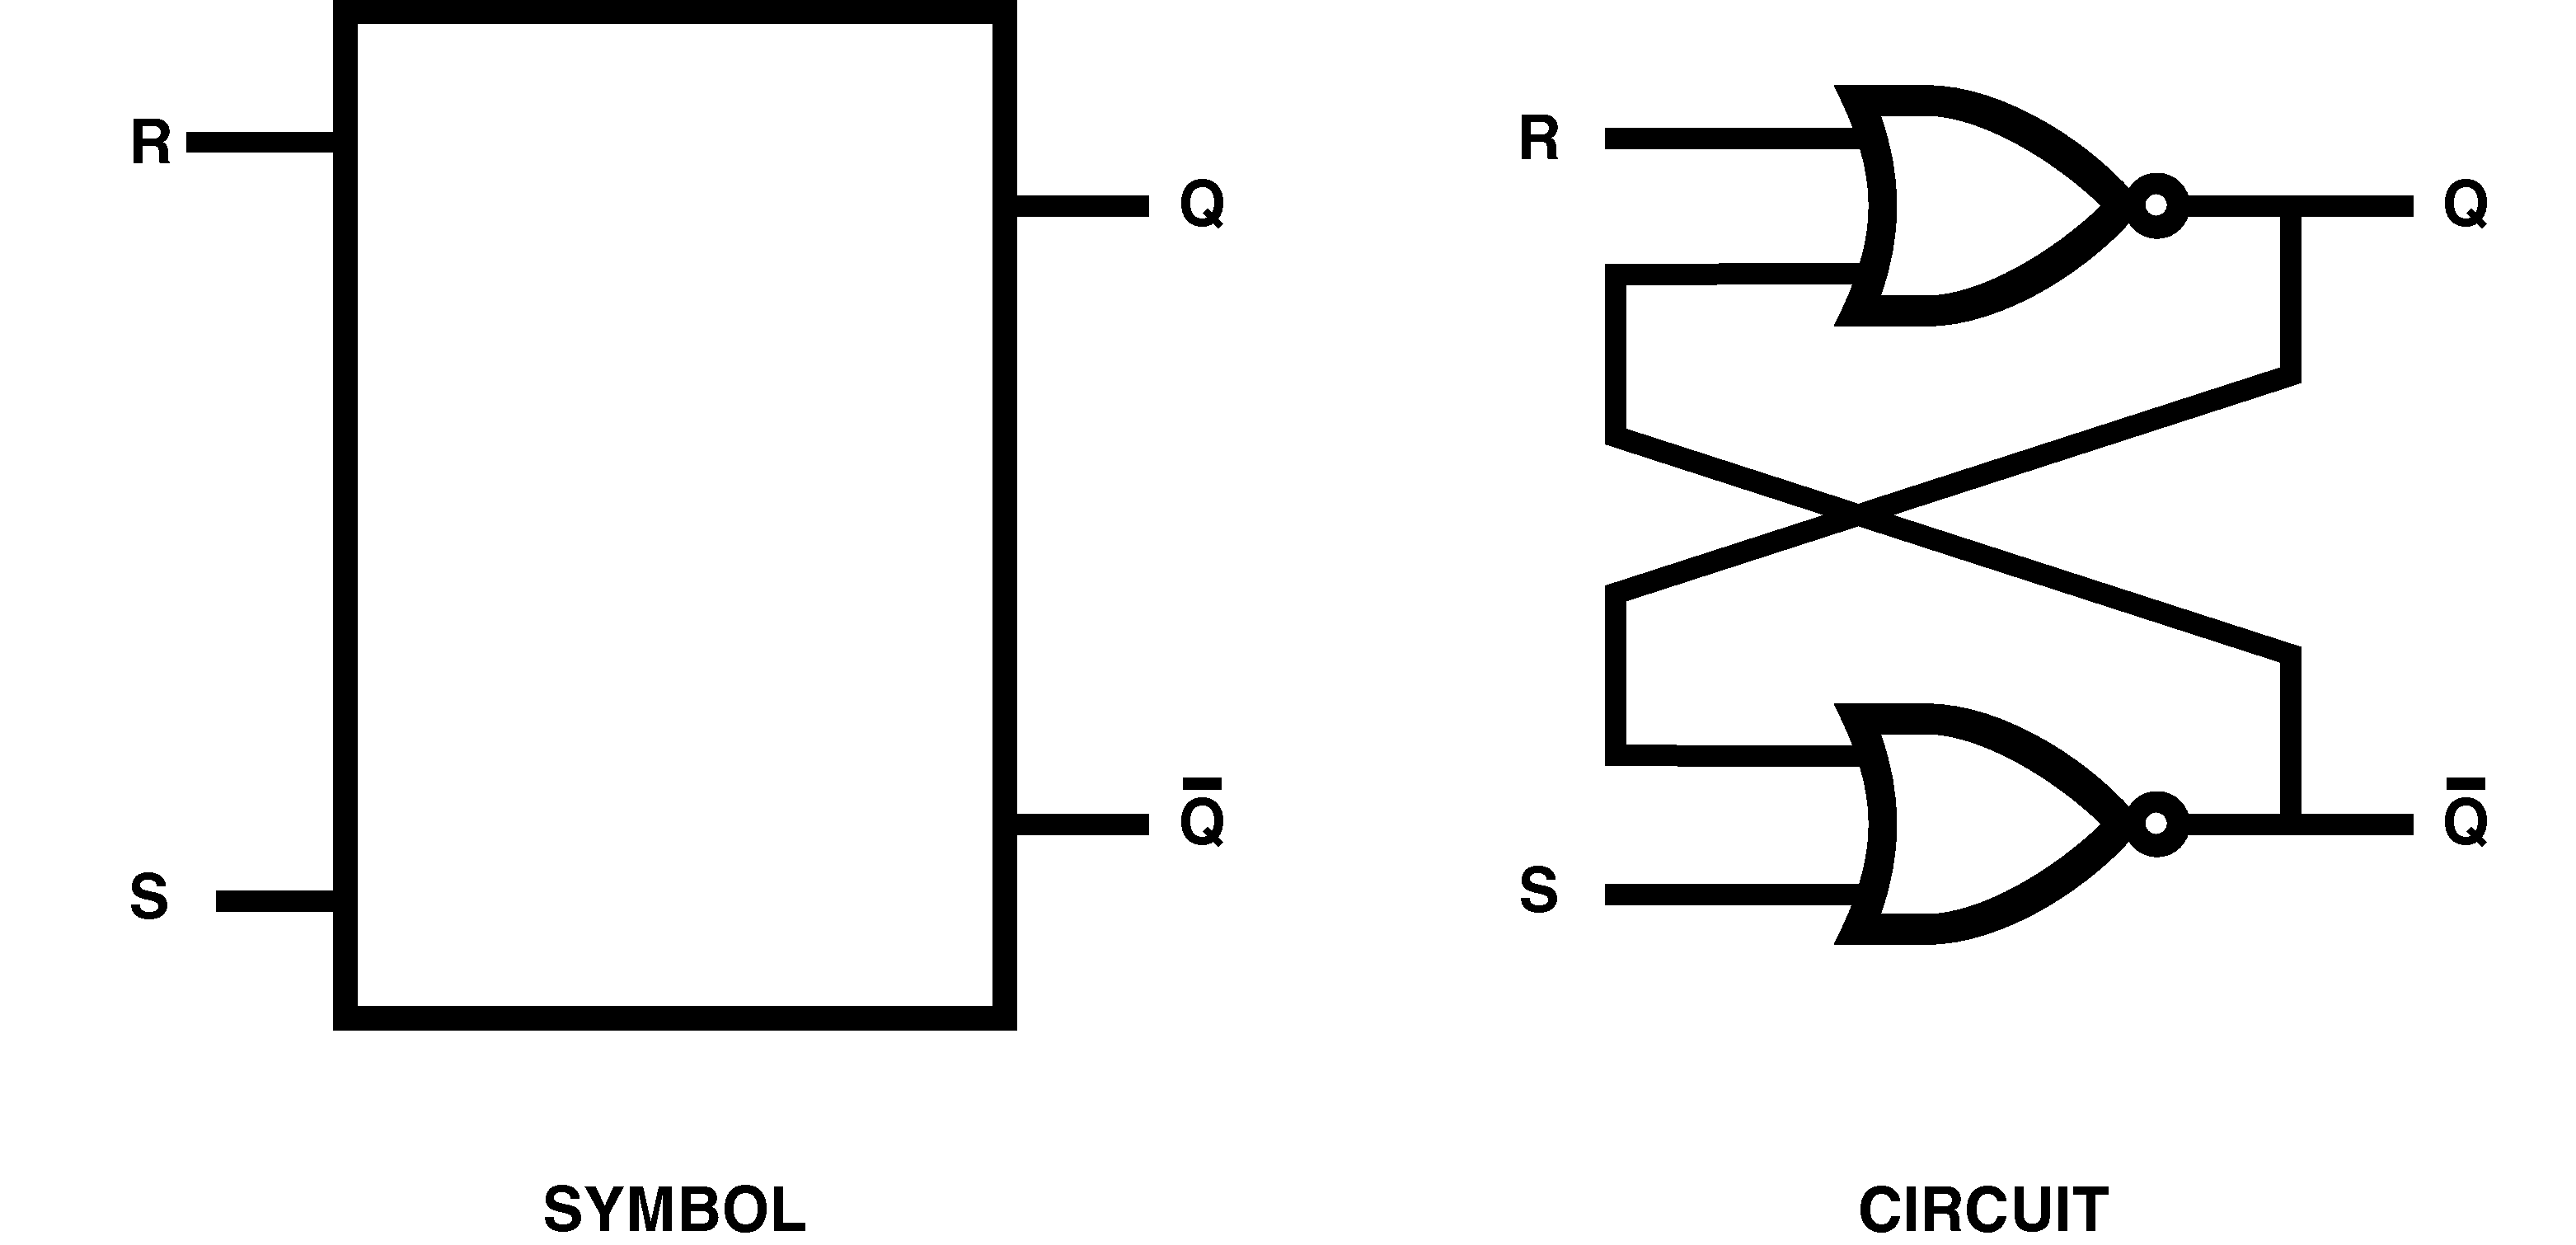
\includegraphics[width=0.95\linewidth]{images/5_memory/flip_flop_sr_nor.pdf}
		\caption{Il flip-flop SR: vedi il \underline{\href{https://www.youtube.com/watch?v=br2pbjAnP2k}{video su youtube}}}
	\end{figure}
	
\end{frame}

\begin{frame}
	\frametitle{Flip-flop SR - NOR Gate}
	 
	\begin{figure}[!htbp] 
		\centering
		%\advance\leftskip-0.25cm
		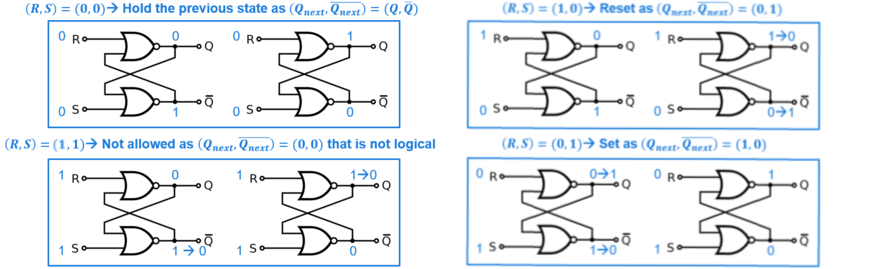
\includegraphics[width=1.0\linewidth]{images/5_memory/flip_flop_sr_nor.png}
		\caption{Il flip-flop SR con NOR, esempi}
	\end{figure}
	
\end{frame}

\begin{frame}

	\frametitle{Flip-flop SR - NOR Gate}

%	\begin{block}{K-means: algoritmo}
		\centering
		\animategraphics[controls={play, step, stop}, height=7cm]{3.0}{images/5_memory/flip_flop_sr_nor/flip_flop_sr_nor-}{0}{15}
		\label{fig:flip_flop_sr_nor}
%	\end{block}

\end{frame}


\subsubsection[Flip-flop SR - NAND Gate]{Flip-flop SR - NAND Gate}
\begin{frame}
	\frametitle{Flip-flop SR - NAND Gate}
	 
	\begin{figure}[!htbp]  
		\centering
		%\advance\leftskip-0.25cm
		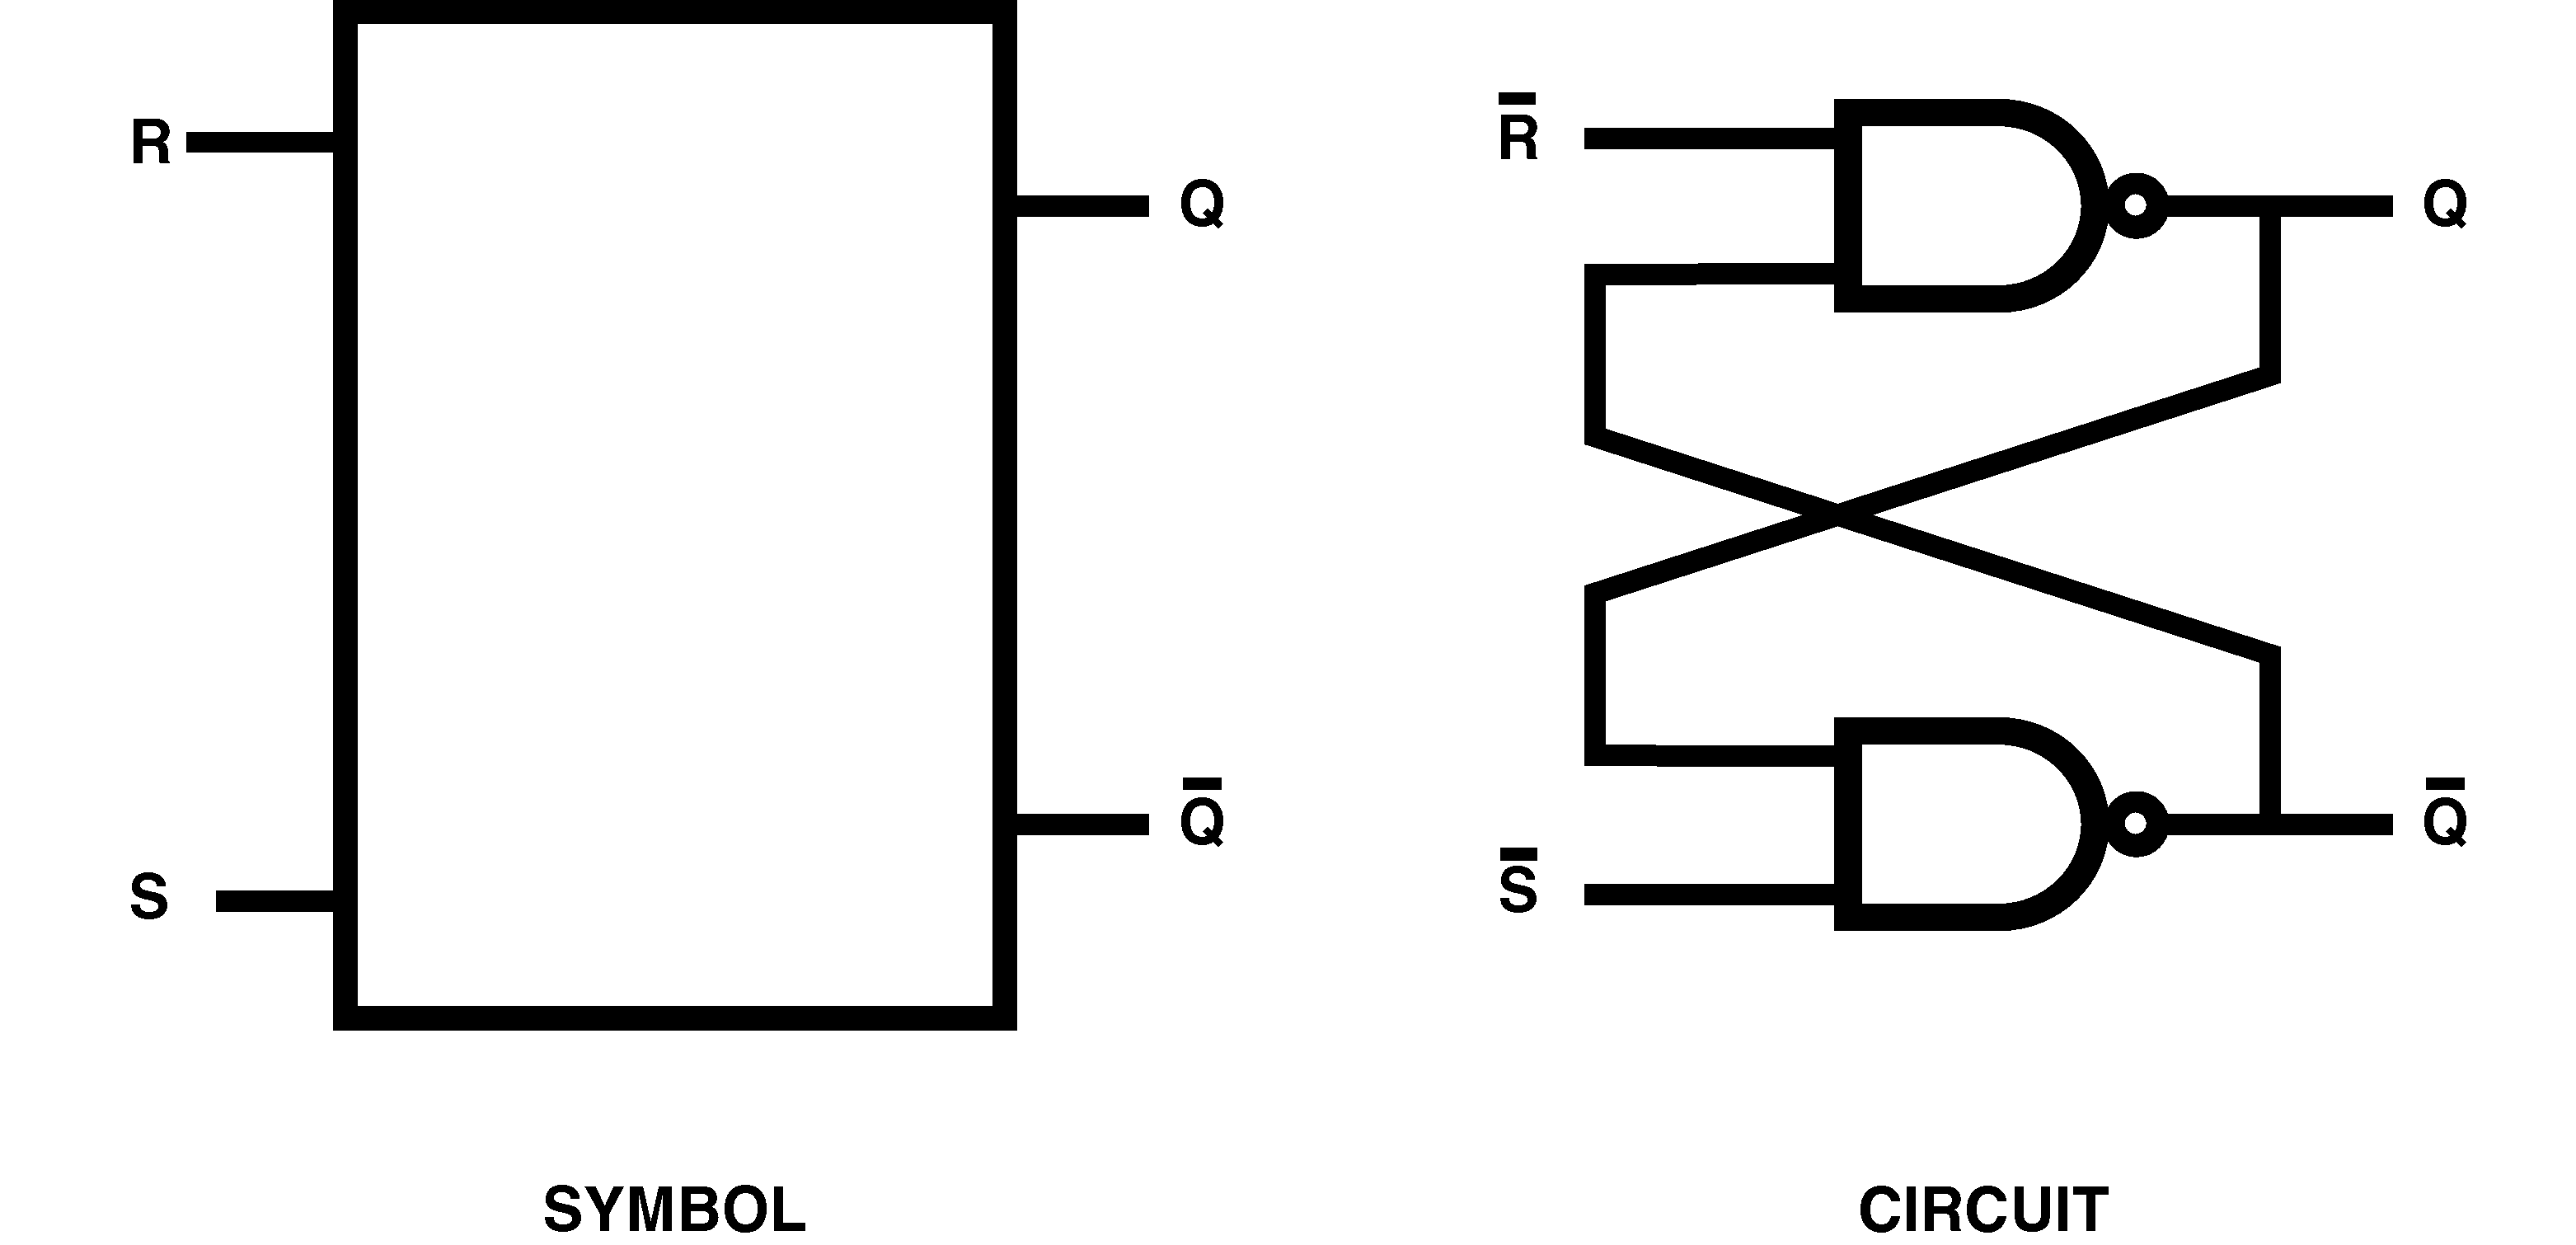
\includegraphics[width=0.95\linewidth]{images/5_memory/flip_flop_sr_nand.pdf}
		\caption{Il flip-flop SR: vedi il \underline{\href{https://www.youtube.com/watch?v=Y9k2oiSJkz4}{video su youtube}}}
	\end{figure}
	
\end{frame}


\subsubsection[Flip-flop D]{Flip-flop D}
\begin{frame}
	\frametitle{Flip-flop D}
	 
	\begin{figure}[!htbp] 
		\centering
		%\advance\leftskip-0.25cm
		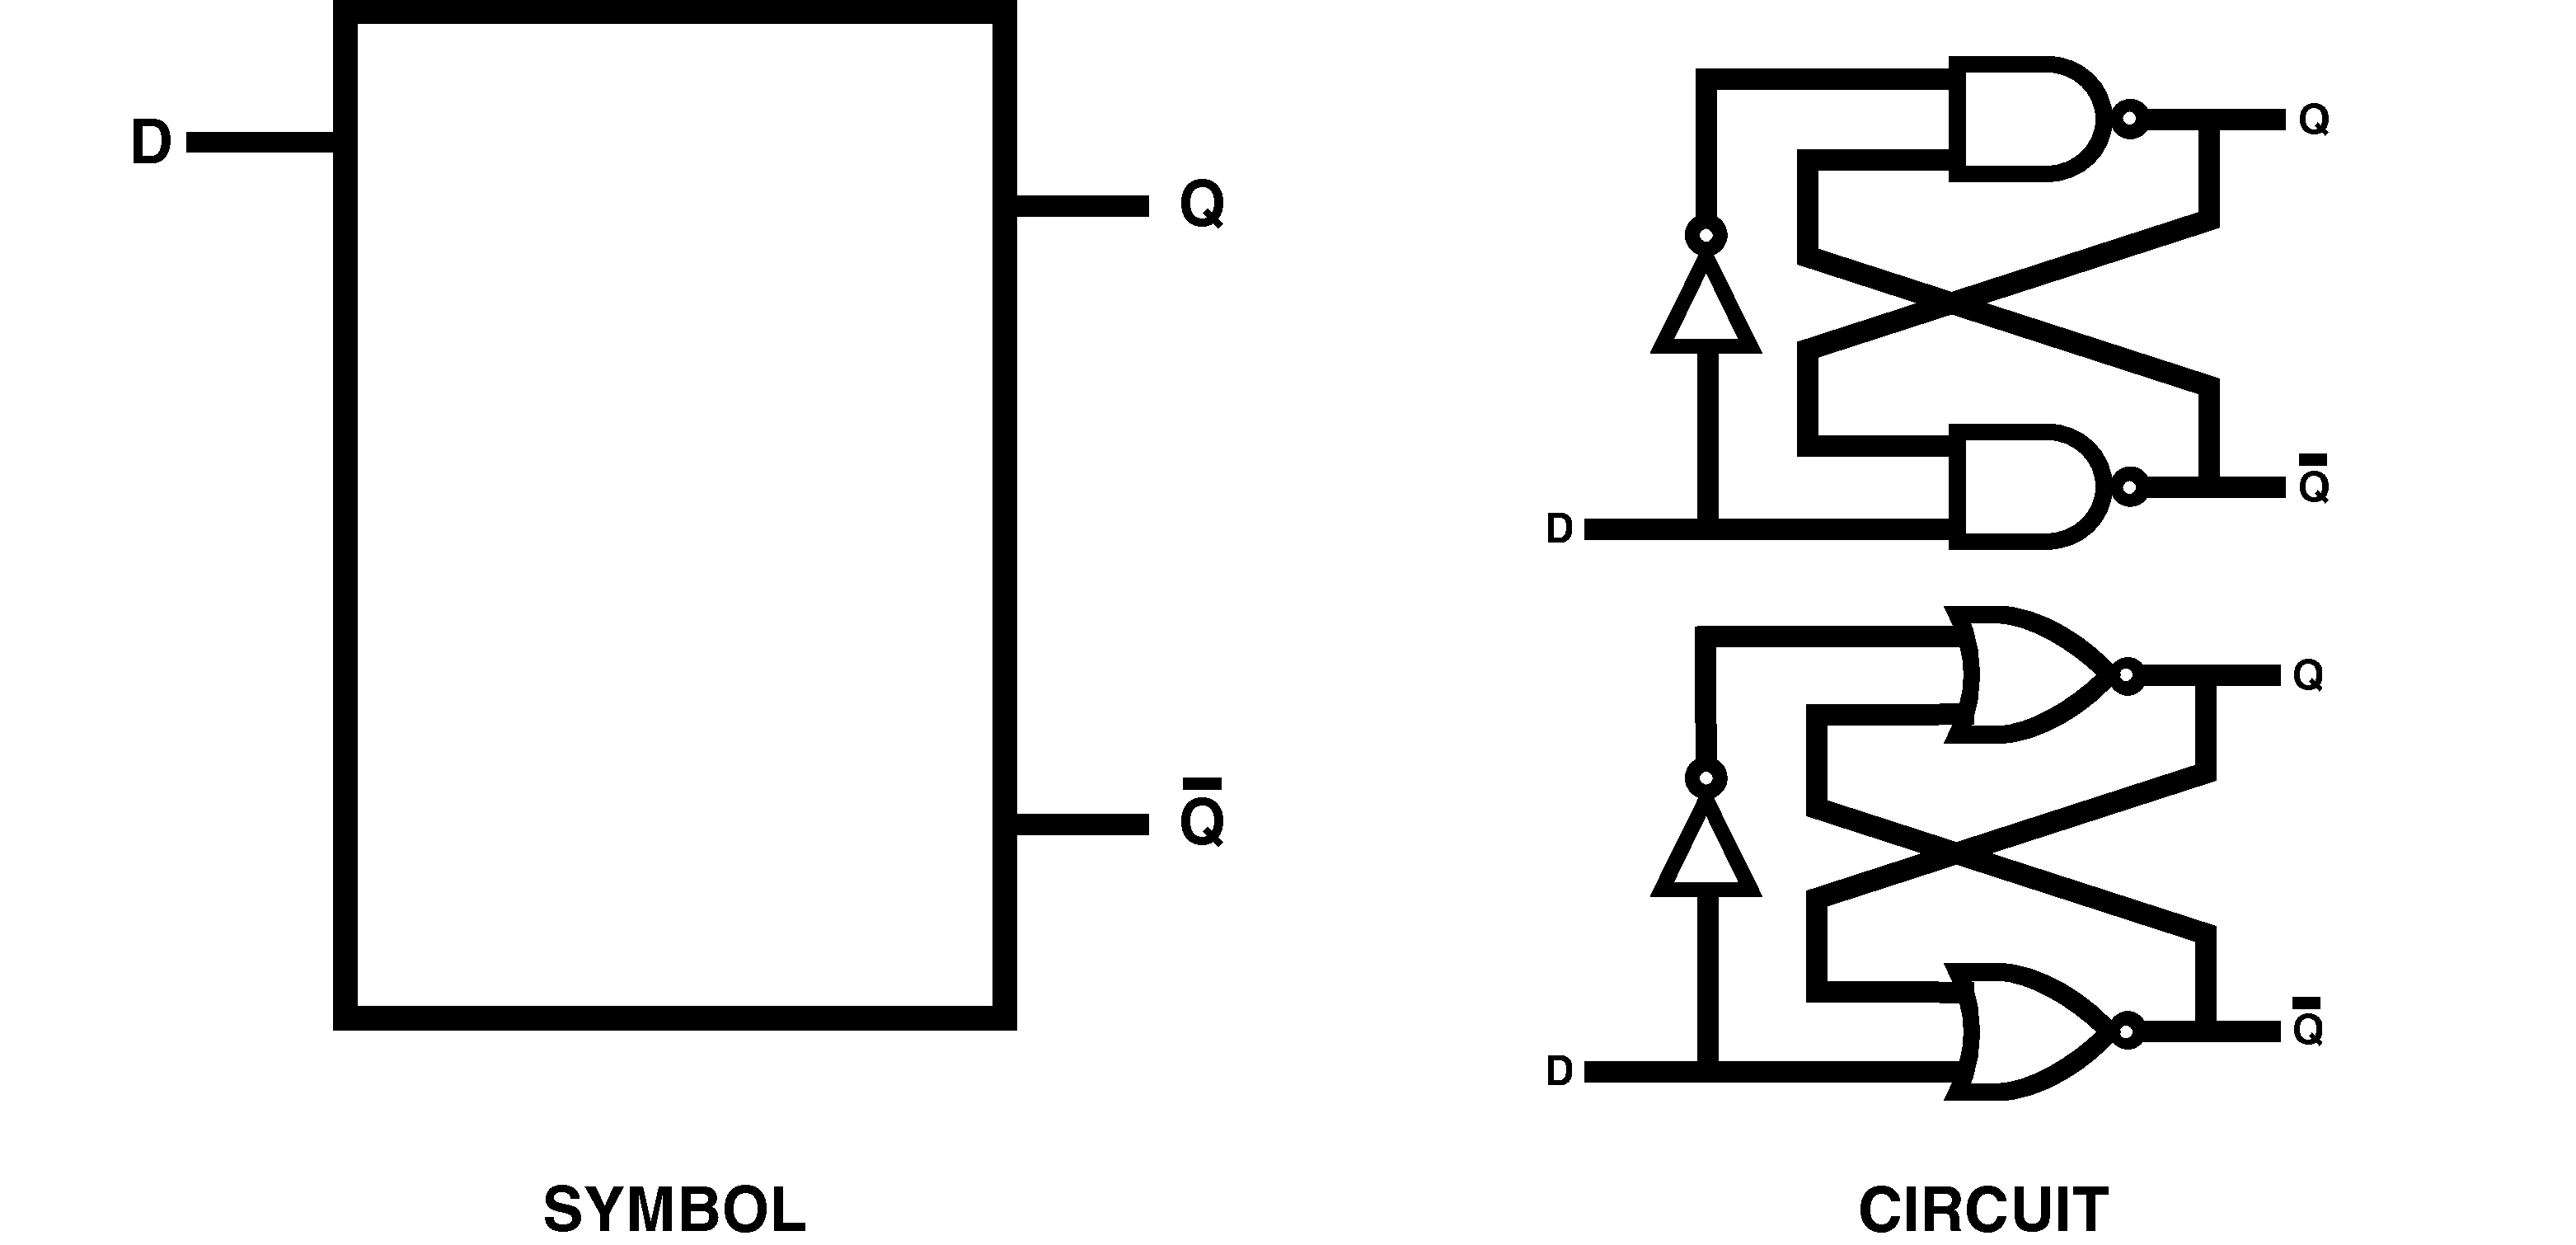
\includegraphics[width=0.75\linewidth]{images/5_memory/flip_flop_d.pdf}
		\caption{Il flip-flop D: è utile per memorizzare un bit di informazione che vengono presentate su una sola line detta "\textbf{Data Line}" (da cui la lettera \textbf{D})}
	\end{figure}
	
\end{frame}




\subsection[La ROM (Read Only Memory)]{La ROM (Read Only Memory)}
\begin{frame}
	\frametitle{La ROM (Read Only Memory)}
	  
	\begin{block}{}
		In elettronica e informatica, una memoria di sola lettura, meglio nota come \textbf{ROM (Read Only Memory)}, indica un tipo di memoria \textit{non volatile} in cui i dati sono memorizzati tramite collegamenti elettronici fisici e stabili.
		
		\begin{figure}[!htbp] 
			\centering
			%\advance\leftskip-0.25cm
			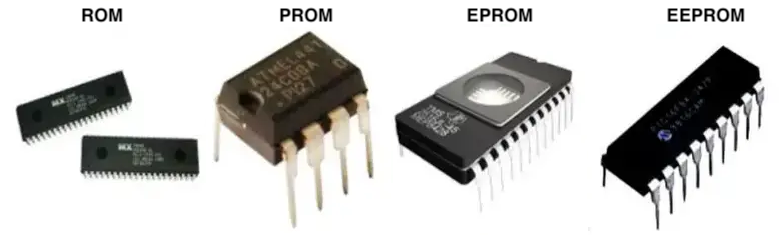
\includegraphics[width=0.80\linewidth]{images/5_memory/roms.png}
			%\caption{Il flip-flop D: è utile per memorizzare un bit di informazione che vengono presentate su una sola line detta "\textbf{Data Line}" (da cui la lettera \textbf{D})}
		\end{figure}
		
		Nonostante il nome suggerisca diversamente alcune ROM possono essere riscritte se sottoposte a specifiche condizioni fisiche.
		
		
		%Contrariamente alla maggior parte delle unità di memoria di massa il suo contenuto non è modificabile durante il normale funzionamento, ma può esserlo, con diverse tecniche, in fase di progettazione, prototipazione o costruzione.
	\end{block}
	
\end{frame}


\subsubsection[Le tipologie di ROM]{Le tipologie di ROM}
\begin{frame}
	\frametitle{Le tipologie di ROM}
	  
	\begin{block}{}
		
		Ogni tipo di ROM è programmata in modo differente a seconda del suo tipo e richiede condizioni speciali per essere cancellata o riscritta.
		
		\begin{figure}[!htbp] 
			\centering
			%\advance\leftskip-0.25cm
			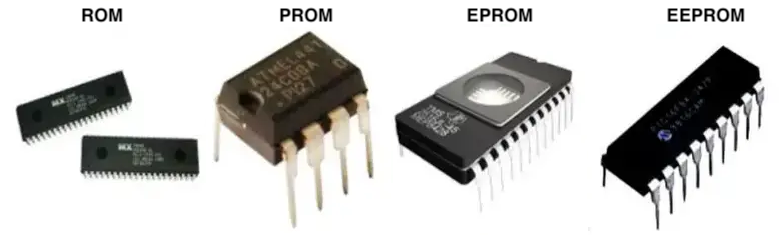
\includegraphics[width=0.80\linewidth]{images/5_memory/roms.png}
			%\caption{Il flip-flop D: è utile per memorizzare un bit di informazione che vengono presentate su una sola line detta "\textbf{Data Line}" (da cui la lettera \textbf{D})}
		\end{figure}
		
		Le  memorie ROM vengono in genere utilizzate per memorizzare programmi e dati di configurazione essenziali per il funzionamento del computer che devono essere memorizzati anche quando il computer è spento.
	\end{block}
	
\end{frame}


\subsubsection[ROM non programmabili]{ROM non programmabili}
\begin{frame}
	\frametitle{Le tipologie di ROM: non programmabili}
	  
	\begin{block}{}
		
		\begin{enumerate}
			\item \textbf{ROM non programmabili}: ROM a maschera, il cui nome deriva dal processo di litografia utilizzato nei circuiti integrati (chip), in cui una fotomaschera permette la creazione del chip. Vengono prodotte già con il programma o i dati "stampati" al loro interno.
		\end{enumerate}
	\end{block}
	
	\begin{columns}			
		\column{0.5\linewidth}
		\begin{figure}[!htbp]
			\centering 
			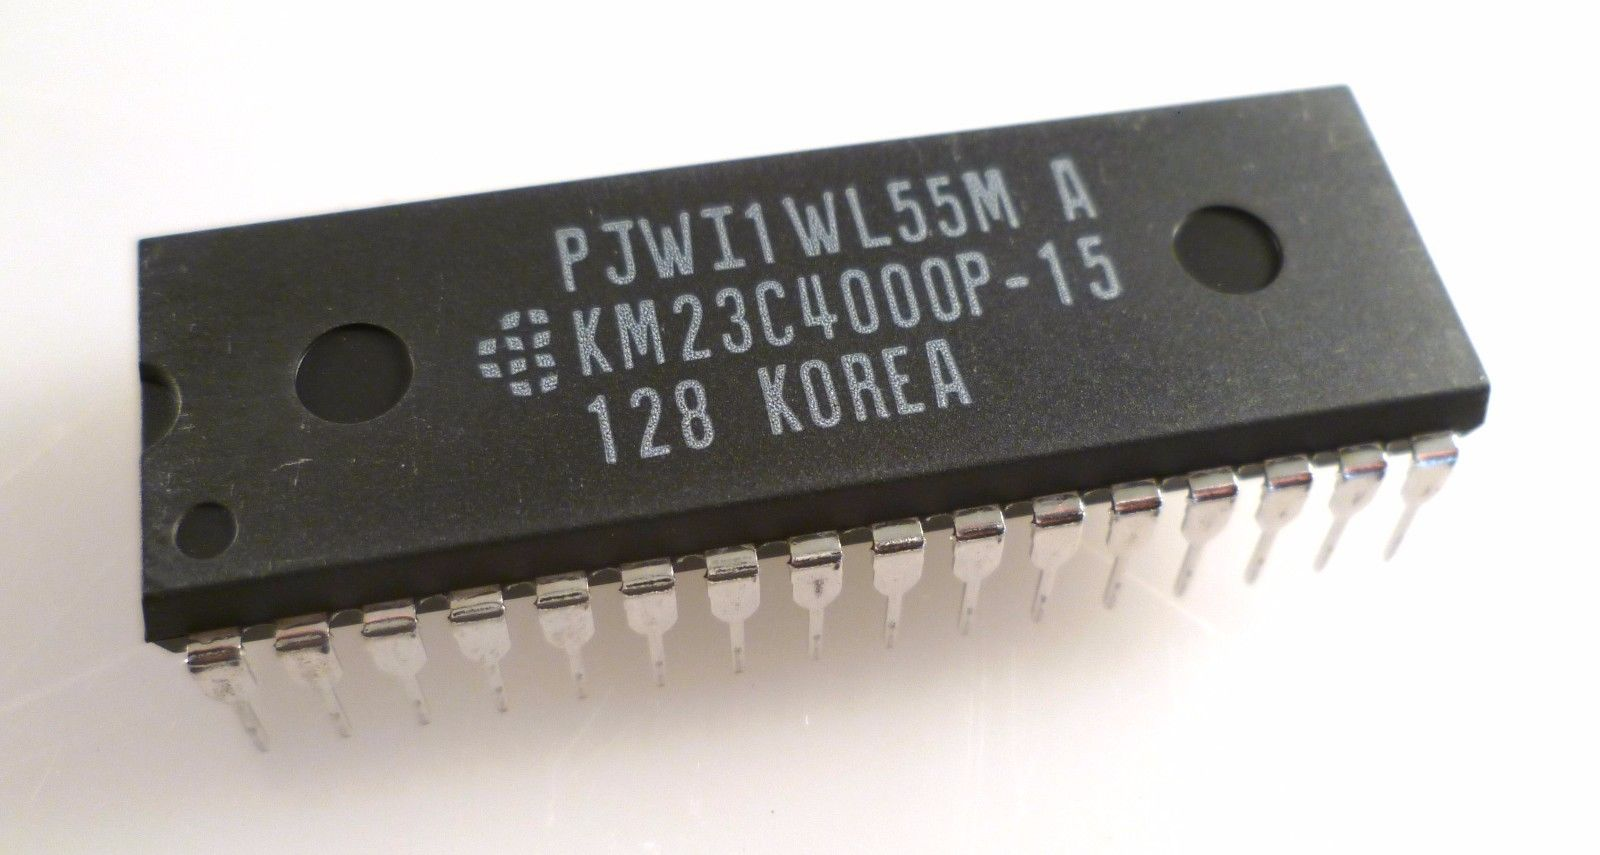
\includegraphics[width=1.0\linewidth]{images/5_memory/rom_mask_top.jpeg}
%				\caption{ROM a maschera}
		\end{figure}
		
		\column{0.5\linewidth}
		\begin{figure}[!htbp]
			\centering 
			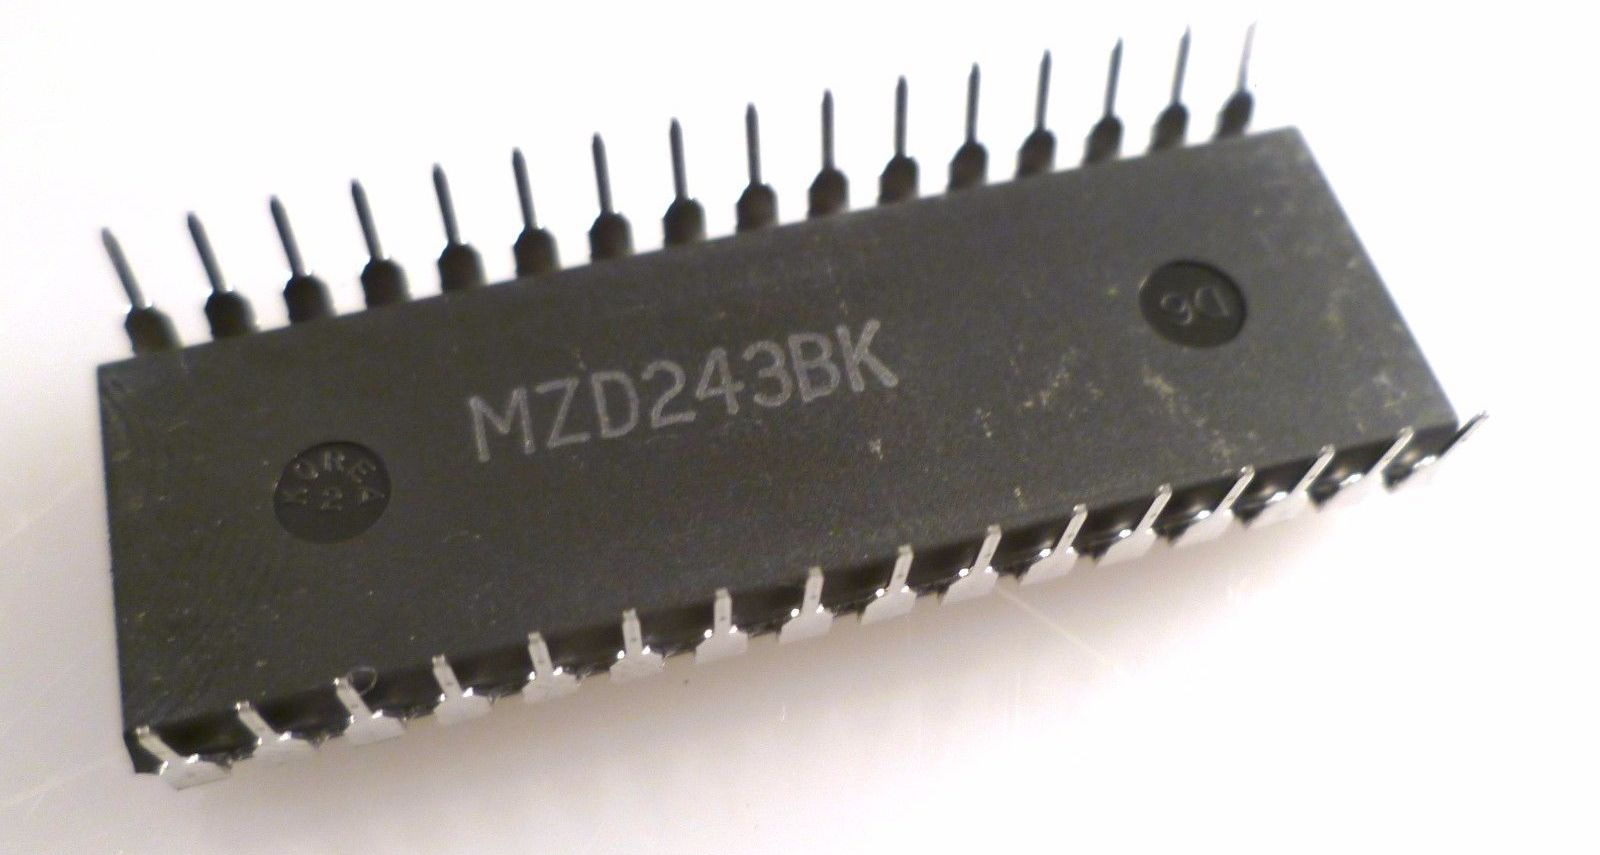
\includegraphics[width=1.0\linewidth]{images/5_memory/rom_mask_bottom.jpeg}
%				\caption{PCI Express: x16, x1, x4, x16} 
		\end{figure}
	\end{columns}
	
\end{frame}


\subsubsection[PROM  (Programmable  ROM)]{PROM  (Programmable  ROM)}
\begin{frame}
	\frametitle{Le tipologie di ROM: PROM}
	  
	\begin{block}{}
		
		\begin{enumerate}
			\setcounter{enumi}{1}
			\item \textbf{PROM  (Programmable  ROM)}: normalmente vengono prodotte vuote al loro interno, possono essere programmate successivamente attraverso appositi \textbf{programmatori di PROM},  tuttavia, una volta programmate, non possono essere più modificate nel  contenuto.
		\end{enumerate}
	\end{block}
	
	\begin{figure}[!htbp] 
		\centering
		%\advance\leftskip-0.25cm
		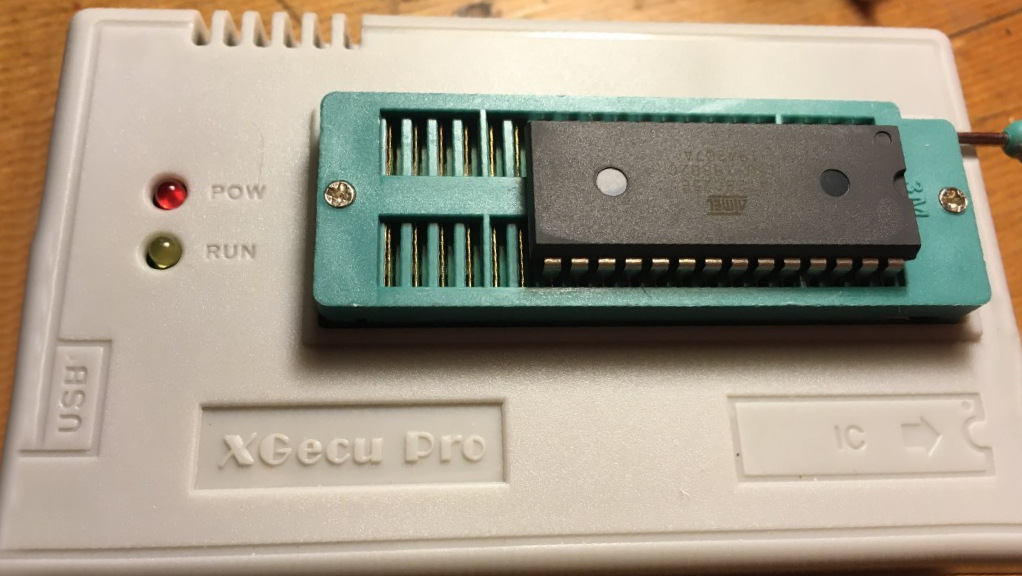
\includegraphics[width=0.7\linewidth]{images/5_memory/prom_programmer.png}
		%\caption{Programmatore di PROM}
	\end{figure}
	
\end{frame}


\subsubsection[EPROM (Erasable Programmable ROM)]{EPROM (Erasable Programmable ROM)}
\begin{frame}
	\frametitle{Le tipologie di ROM: EPROM}
	  
	\begin{block}{}

		\begin{enumerate}
			\setcounter{enumi}{2}
			\item \textbf{EPROM (Erasable Programmable ROM)}: normalmente sono vuote al loro interno e possono  essere  programmate  attraverso appositi programmatori di EPROM. A differenza delle PROM, la programmazione può avvenire più volte, a patto di cancellare la vecchia programmazione tramite raggi UV (ultravioletti).
		\end{enumerate}
		
	\end{block}
	
	\begin{columns}			
		\column{0.5\linewidth}
		\begin{figure}[!htbp]
			\centering 
			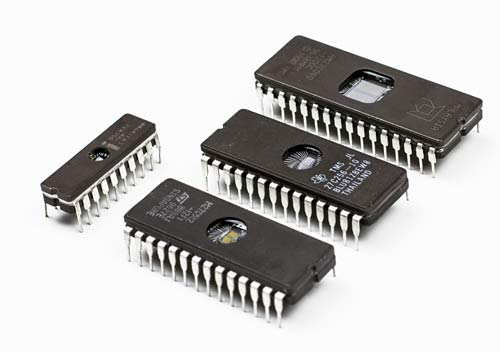
\includegraphics[width=1.0\linewidth]{images/5_memory/eproms.jpg }
%				\caption{ROM a maschera}
		\end{figure}
		
		\column{0.5\linewidth}
		\begin{figure}[!htbp]
			\centering 
			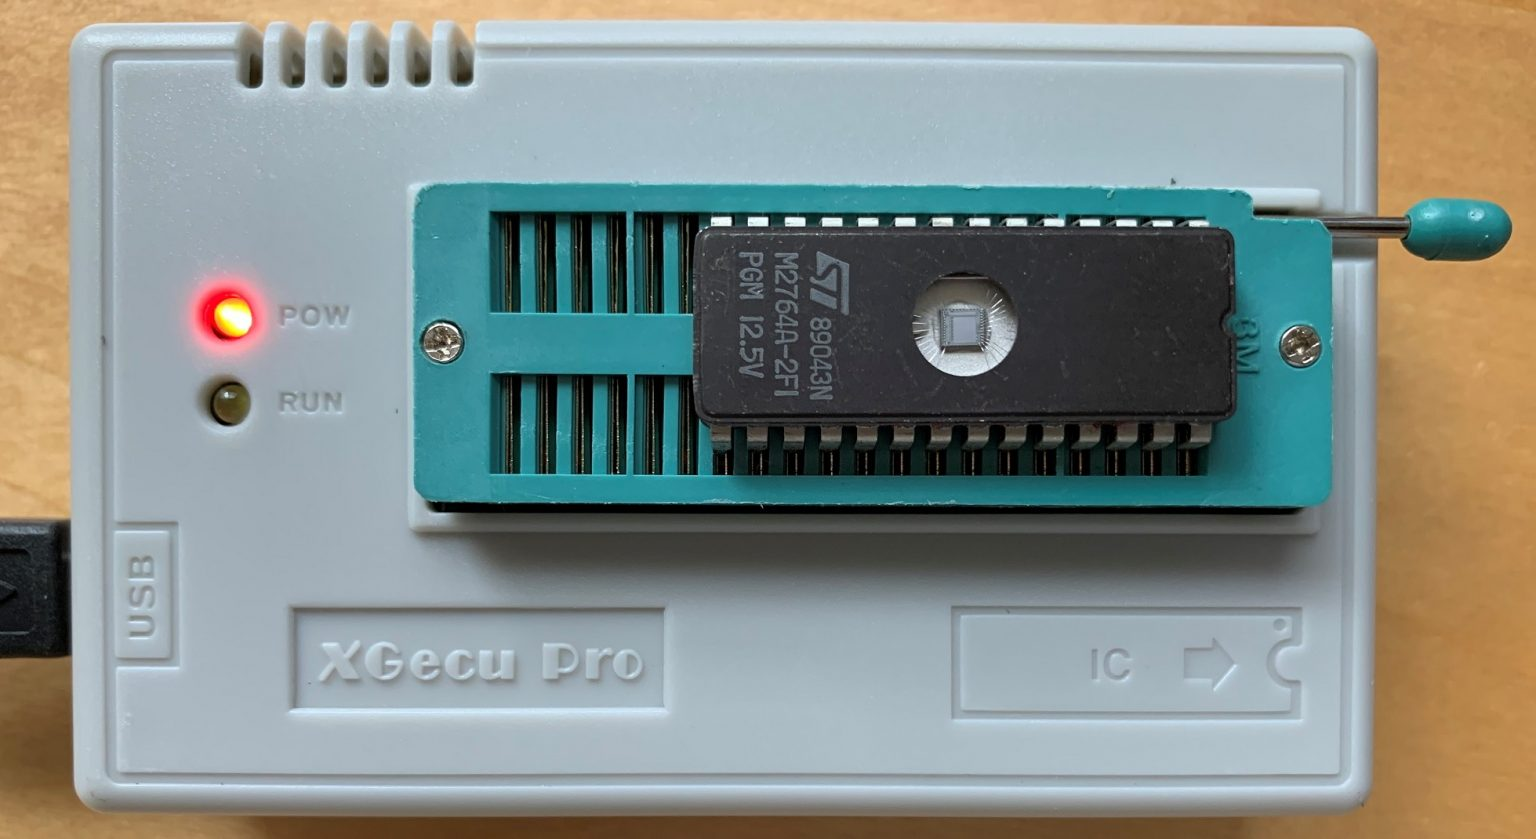
\includegraphics[width=1.0\linewidth]{images/5_memory/eprom_programmer.jpg}
%				\caption{PCI Express: x16, x1, x4, x16} 
		\end{figure}
	\end{columns}
	
	\begin{figure}[!htbp] 
		\centering
		%\advance\leftskip-0.25cm
		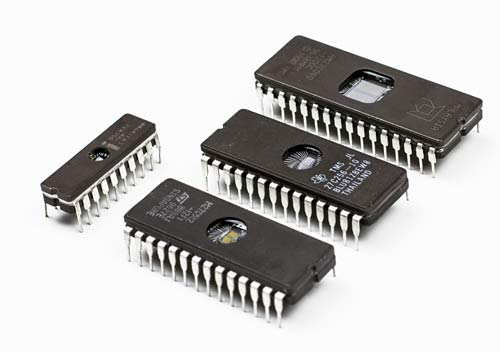
\includegraphics[width=0.5\linewidth]{images/5_memory/eproms.jpg }
		%\caption{PROM: nota la finestrella posta nella parte superiore del  circuito, che permette di ricevere i raggi UV}
	\end{figure}
	
\end{frame}



\begin{frame}
	\frametitle{Le tipologie di ROM: EPROM}
	 
	\begin{figure}[!htbp] 
		\centering
		%\advance\leftskip-0.25cm
		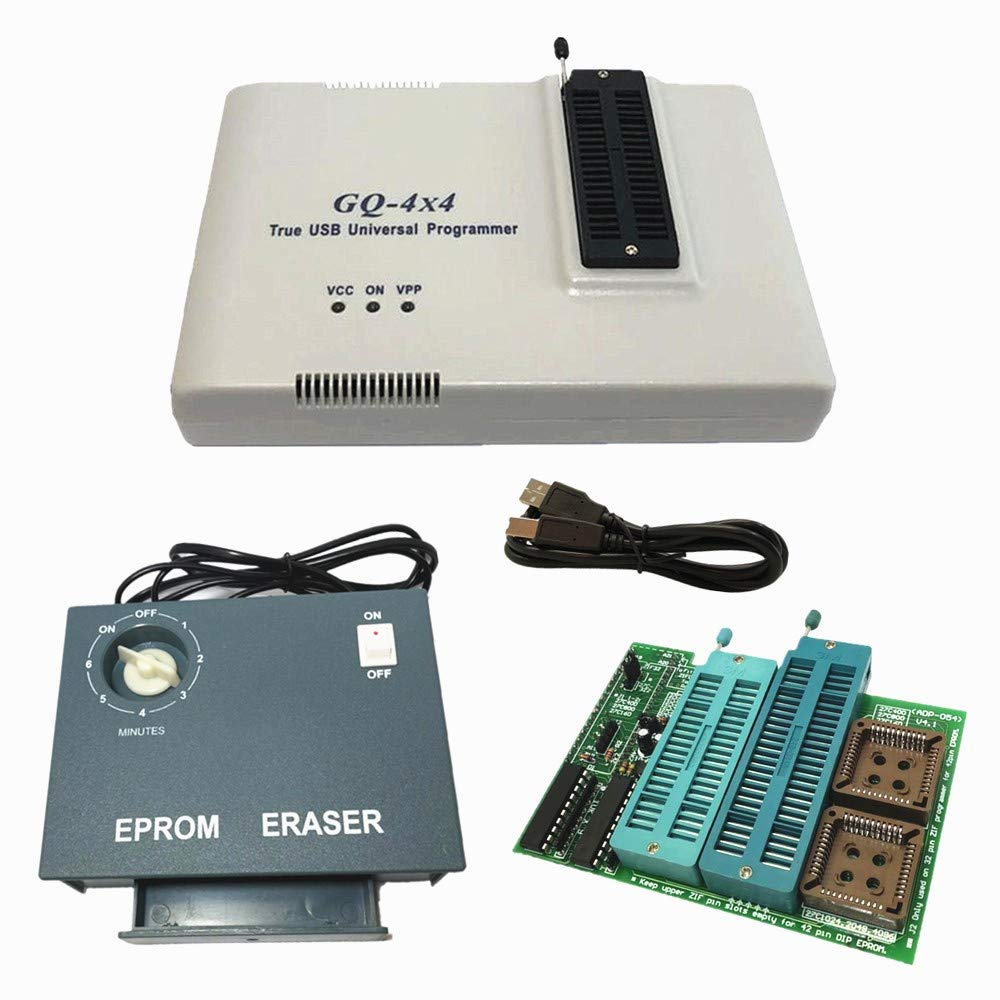
\includegraphics[width=0.6\linewidth]{images/5_memory/eprom_writer_eraser.jpg}
		%\caption{PROM: nota la finestrella posta nella parte superiore del  circuito, che permette di ricevere i raggi UV}
	\end{figure}
	
\end{frame}


\begin{frame}
	\frametitle{Le tipologie di ROM: EPROM}
	 
	\begin{figure}[!htbp] 
		\centering
		%\advance\leftskip-0.25cm
		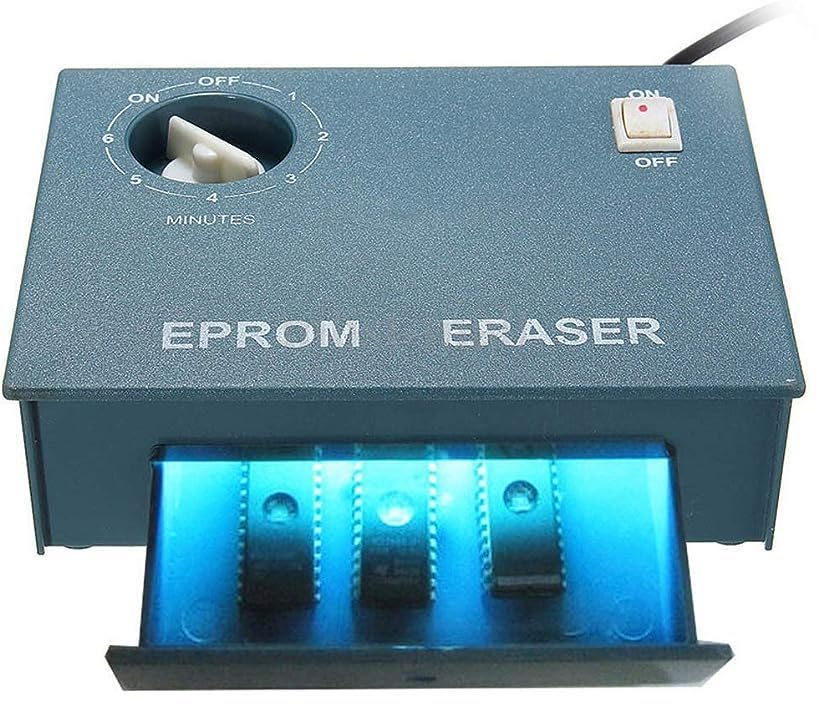
\includegraphics[width=0.6\linewidth]{images/5_memory/eprom_eraser.jpg}
		%\caption{PROM: nota la finestrella posta nella parte superiore del  circuito, che permette di ricevere i raggi UV}
	\end{figure}
	
\end{frame}



\subsubsection[EEPROM (Electrical  Erasable  Programmable  ROM)]{EEPROM (Electrical  Erasable  Programmable  ROM)}
\begin{frame}
	\frametitle{Le tipologie di ROM: EEPROM}
	  
	\begin{block}{}

		\begin{enumerate}
			\setcounter{enumi}{3}
			\item \textbf{EEPROM (Electrical  Erasable  Programmable  ROM)}: identiche alle EPROM, dalle quali differiscono solo per il fatto che la cancellazione della vecchia programmazione è realizzata più semplicemente tramite un flusso di corrente elettrica. 
		\end{enumerate}
		
	\end{block}
	
	\begin{figure}[!htbp] 
		\centering
		%\advance\leftskip-0.25cm
		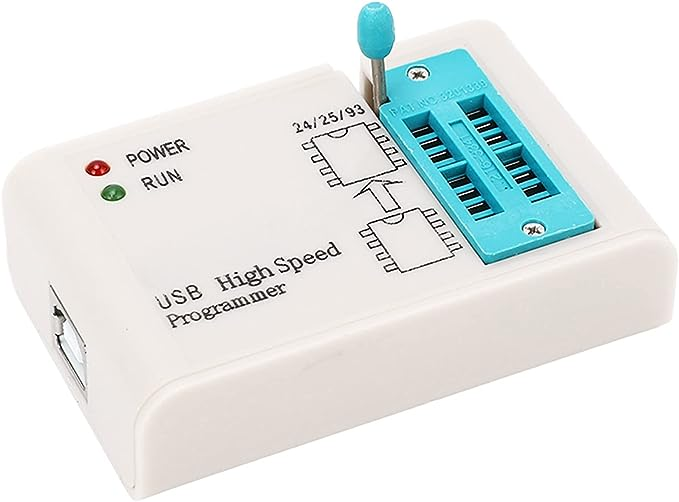
\includegraphics[width=0.55\linewidth]{images/5_memory/eeprom_programmer.jpg}
		%\caption{Programmatore di PROM}
	\end{figure}
	
\end{frame}




\subsection[La RAM (Random Access Memory)]{La RAM (Random Access Memory)}
\begin{frame}
	\frametitle{La RAM (Random Access Memory)}
	  
	\begin{block}{}
		La \textbf{memoria ad accesso casuale} o \textbf{RAM} (Random Access Memory), è un tipo di memoria volatile caratterizzata dal permettere l'accesso diretto a qualunque indirizzo di memoria con le stesse identiche tempistiche.
		
		\begin{figure}[!htbp]
			\centering
			%\advance\leftskip-0.25cm
			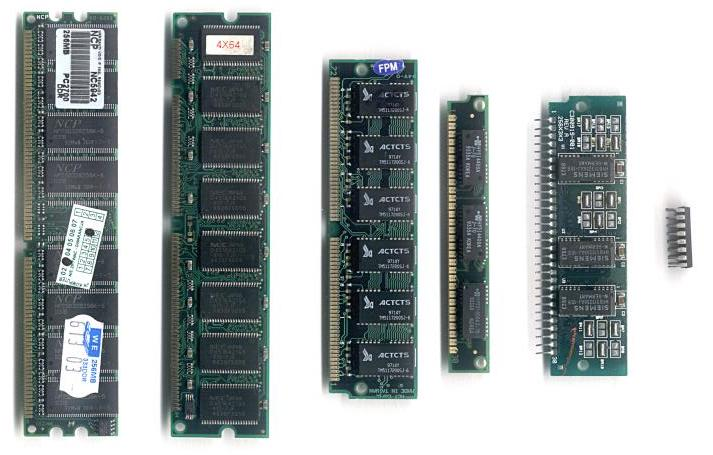
\includegraphics[width=0.58\linewidth]{images/5_memory/ram.jpg}
%			\caption{RAM (Random Access Memory)}
			\label{fig:memory_ram}
		\end{figure}
	\end{block}
\end{frame}



% http://www.brescianet.com/appunti/infobase/pc_C.htm
\subsubsection[I tipi di RAM]{I tipi di RAM}
\begin{frame}
	\frametitle{I tipi di RAM}
	  
	\begin{block}{}
		%La RAM si contrappone alla memoria ad accesso sequenziale, in cui i dati sono disposti in modo sequenziale e per accedervi è necessario scorrere su tutti i dati precedenti.\\~\\
		
		Possiamo distinguere le RAM in diverse tipologie:
		\begin{itemize}
			\item Le \textbf{DRAM} (dynamic RAM): tempo di accesso 20-70ns con refresh. Sono \textbf{poco costose}. Sono principalmente utilizzate per la \textit{\underline{memoria centrale}} del computer.
			\item Le \textbf{SDRAM} (synchronous dynamic RAM): evoluzione della DRAM, sincrona rispetto al BUS di sistema, ovvero utilizza un segnale di clock esterno per la sincronizzazione delle operazioni di I/O; questo permette un incremento delle prestazioni e una maggiore efficienza.
			\item Le \textbf{SRAM} (static RAM): tempo di accesso 5-10ns senza refresh. Sono \textbf{rapide ma costose}. Sono soprattutto utilizzate per le \textit{\underline{memorie cache}} del processore.
			\item ... \textbf{FeRAM}, \textbf{memorie a cambiamento di fase} ...
			%\item Le \textbf{FeRAM} (ferroelectric dynamic RAM): mantiene i dati senza l'ausilio del refresh di sistema. Utilizzano un materiale denominato ferroelettrico che ha la capacità di mantenere la propria polarizzazione anche dopo esser scollegato dalla fonte energetica.
		\end{itemize}
	\end{block}
\end{frame}


\subsubsection[La DRAM: dynamic RAM]{La DRAM: dynamic RAM}
\begin{frame}
	\frametitle{La DRAM: dynamic RAM}
	  
	\begin{block}{}
		La memoria dinamica DRAM è costituita da centinaia di migliaia di piccoli \textbf{condensatori} (sorta di serbatoio elettrico) che immagazzinano delle cariche. Una volta caricato, lo stato software del condensatore è pari a 1, in caso contrario è a 0, il che significa che ogni condensatore rappresenta un bit della memoria.\\~\\
		Dato che i condensatori si scaricano, bisogna costantemente ricaricarli (il termine esatto è \textbf{refresh}) ad un intervallo di tempo regolare detto \textbf{ciclo di refresh}. Le memorie DRAM hanno ad esempio bisogno di cicli di refresh ogni 15 nanosecondi (ns) circa.\\~\\
		
		Oltre a comportare un certo dispendio di energia rendono più lenta la memoria in quanto, mentre si sta eseguendo il refreshing, non è possibile accedervi.
	\end{block}
\end{frame}

\begin{frame}
	\frametitle{La DRAM: dynamic RAM}
	  
	\begin{block}{}
		È importante sottolineare come l'operazione di lettura sia distruttiva, in quanto nel momento in cui un dato viene letto viene anche perso; risulta quindi necessaria la sua riscrittura immediata e questa porta a uno spreco di tempo.\\~\\
		Ogni condensatore è accoppiato ad un transistor (di tipo MOS) che permette di "recuperare" (leggere) o di modificare lo stato del condensatore. Questi transistor sono disposti sotto forma di tabella (matrice). I punti di memoria vengono indicati con una linea e una colonna.
	\end{block}
	
	\begin{columns}			
		\column{0.5\linewidth}
		\begin{figure}[!htbp]
			\centering 
			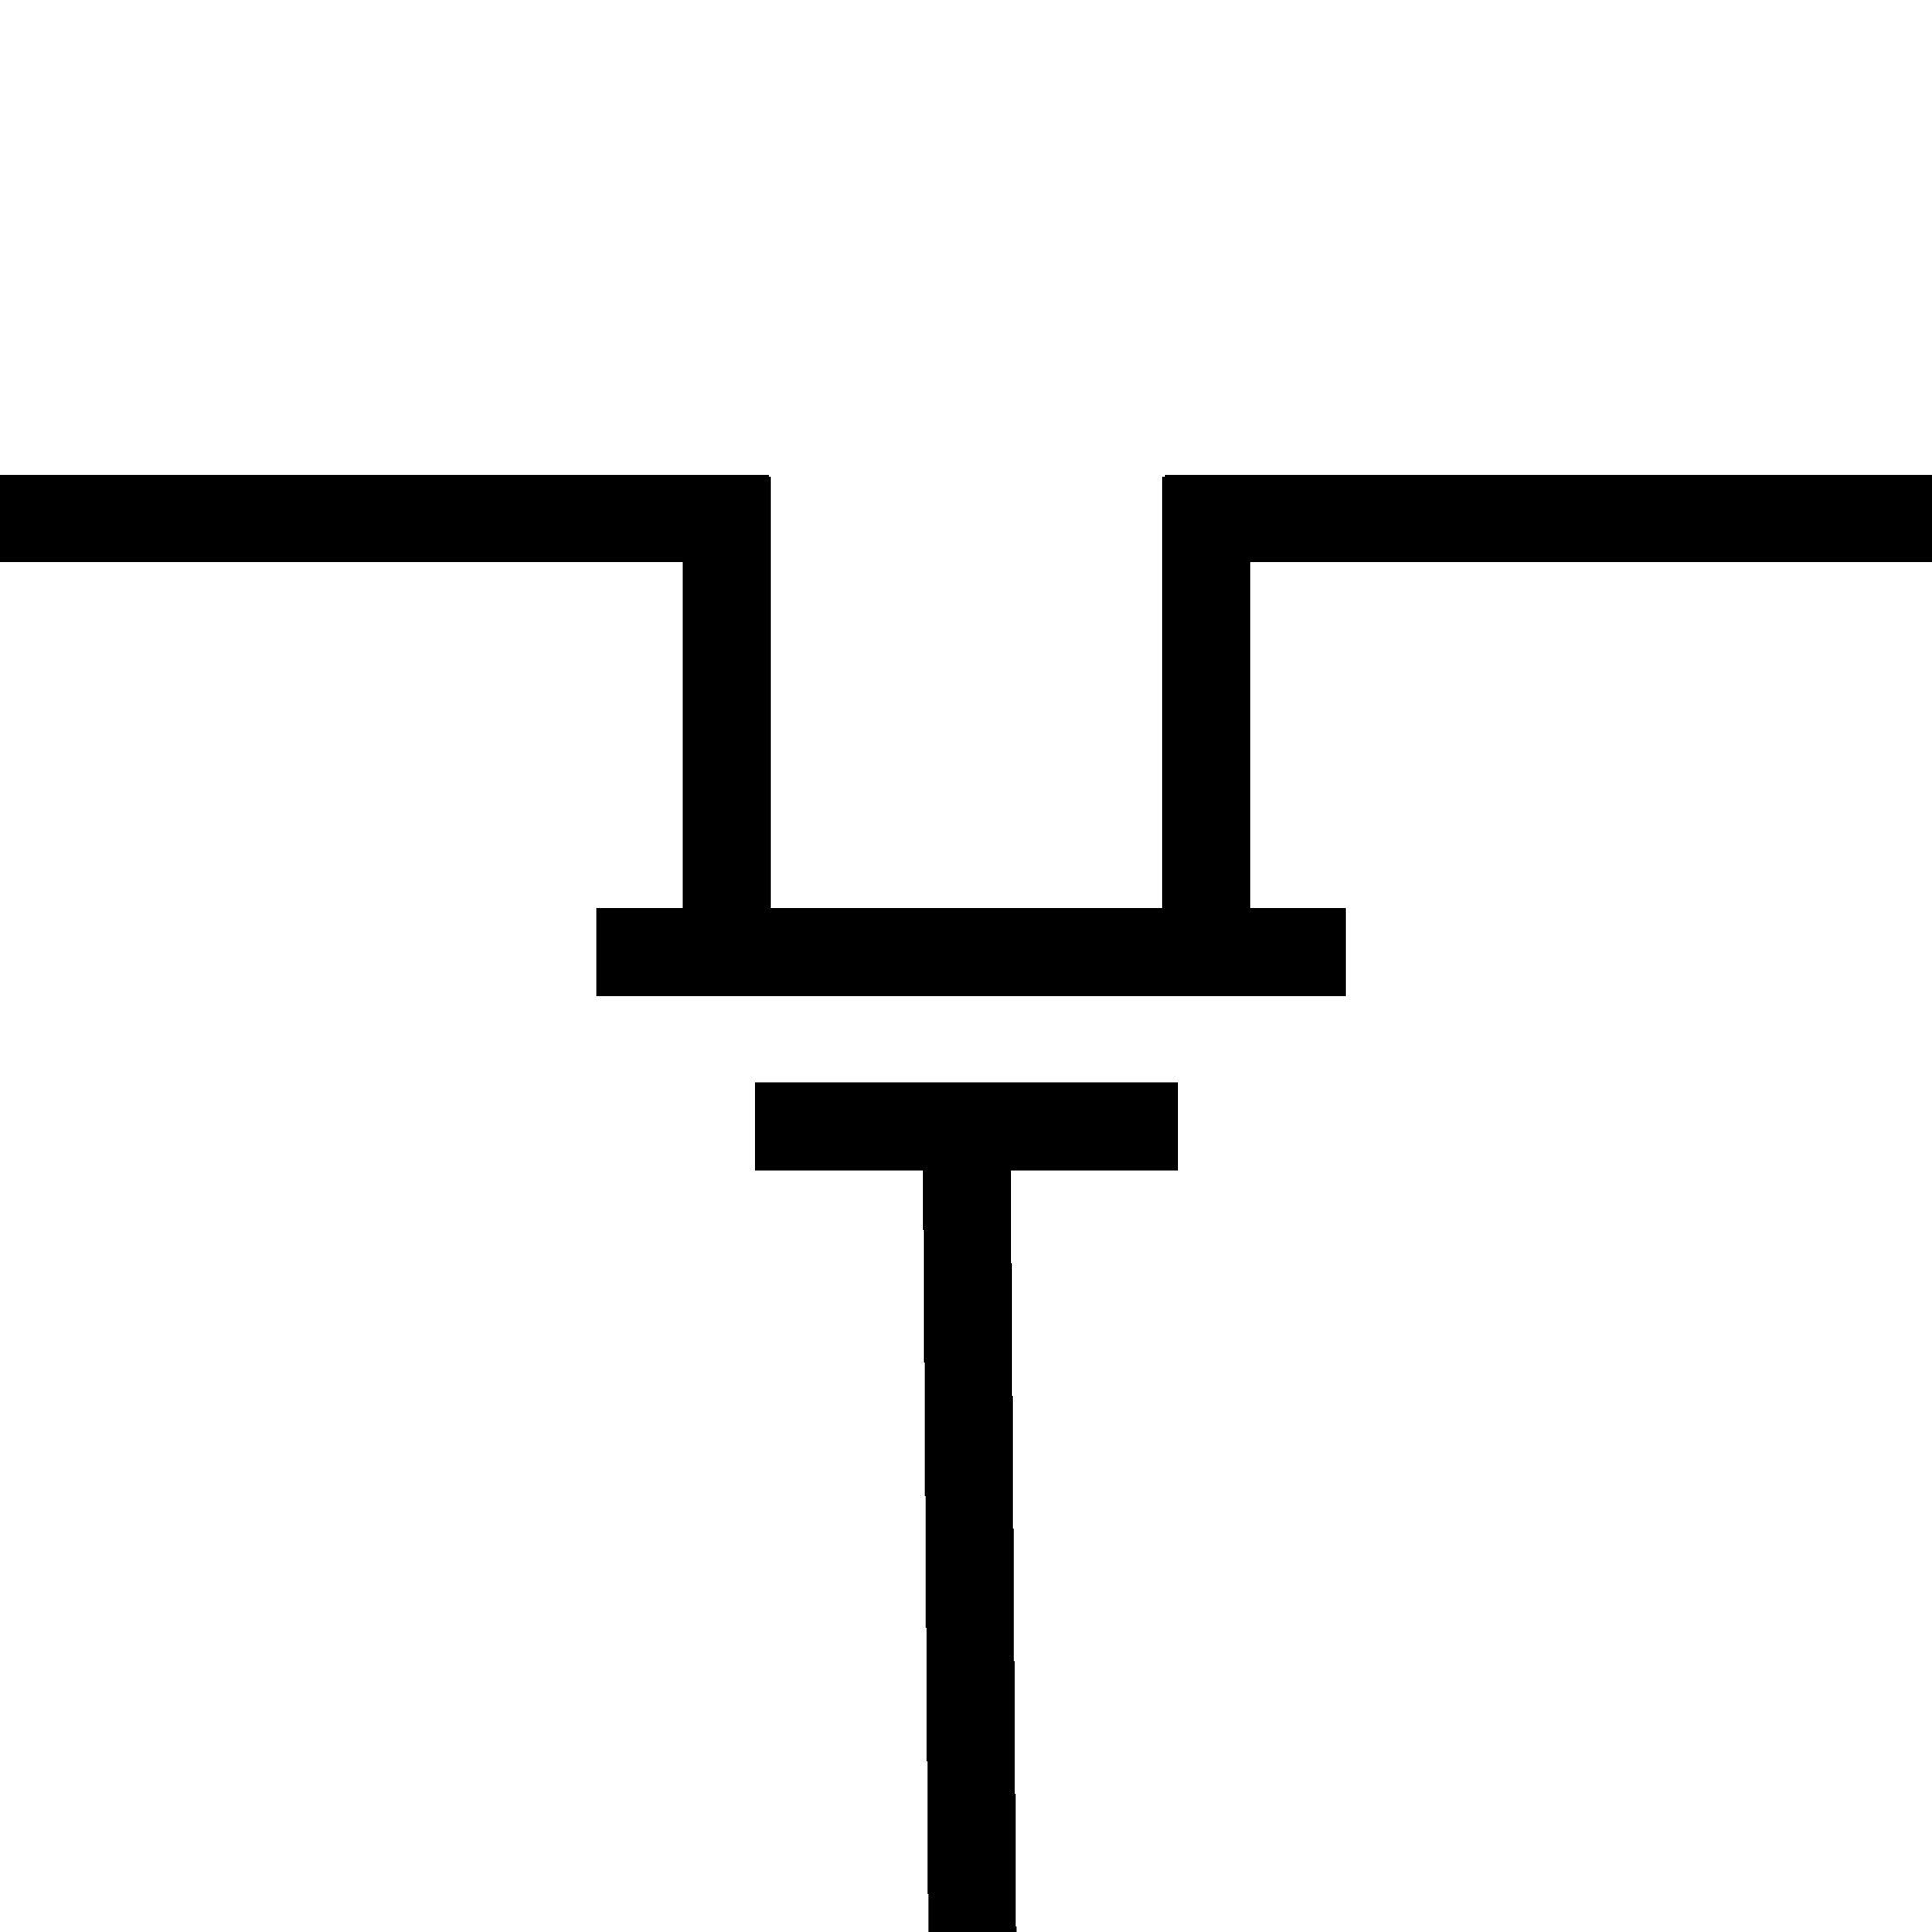
\includegraphics[width=0.15\linewidth]{images/5_memory/transistor.pdf}
				\caption{Transistor}
		\end{figure}
		
		\column{0.5\linewidth}
		\begin{figure}[!htbp]
			\centering 
			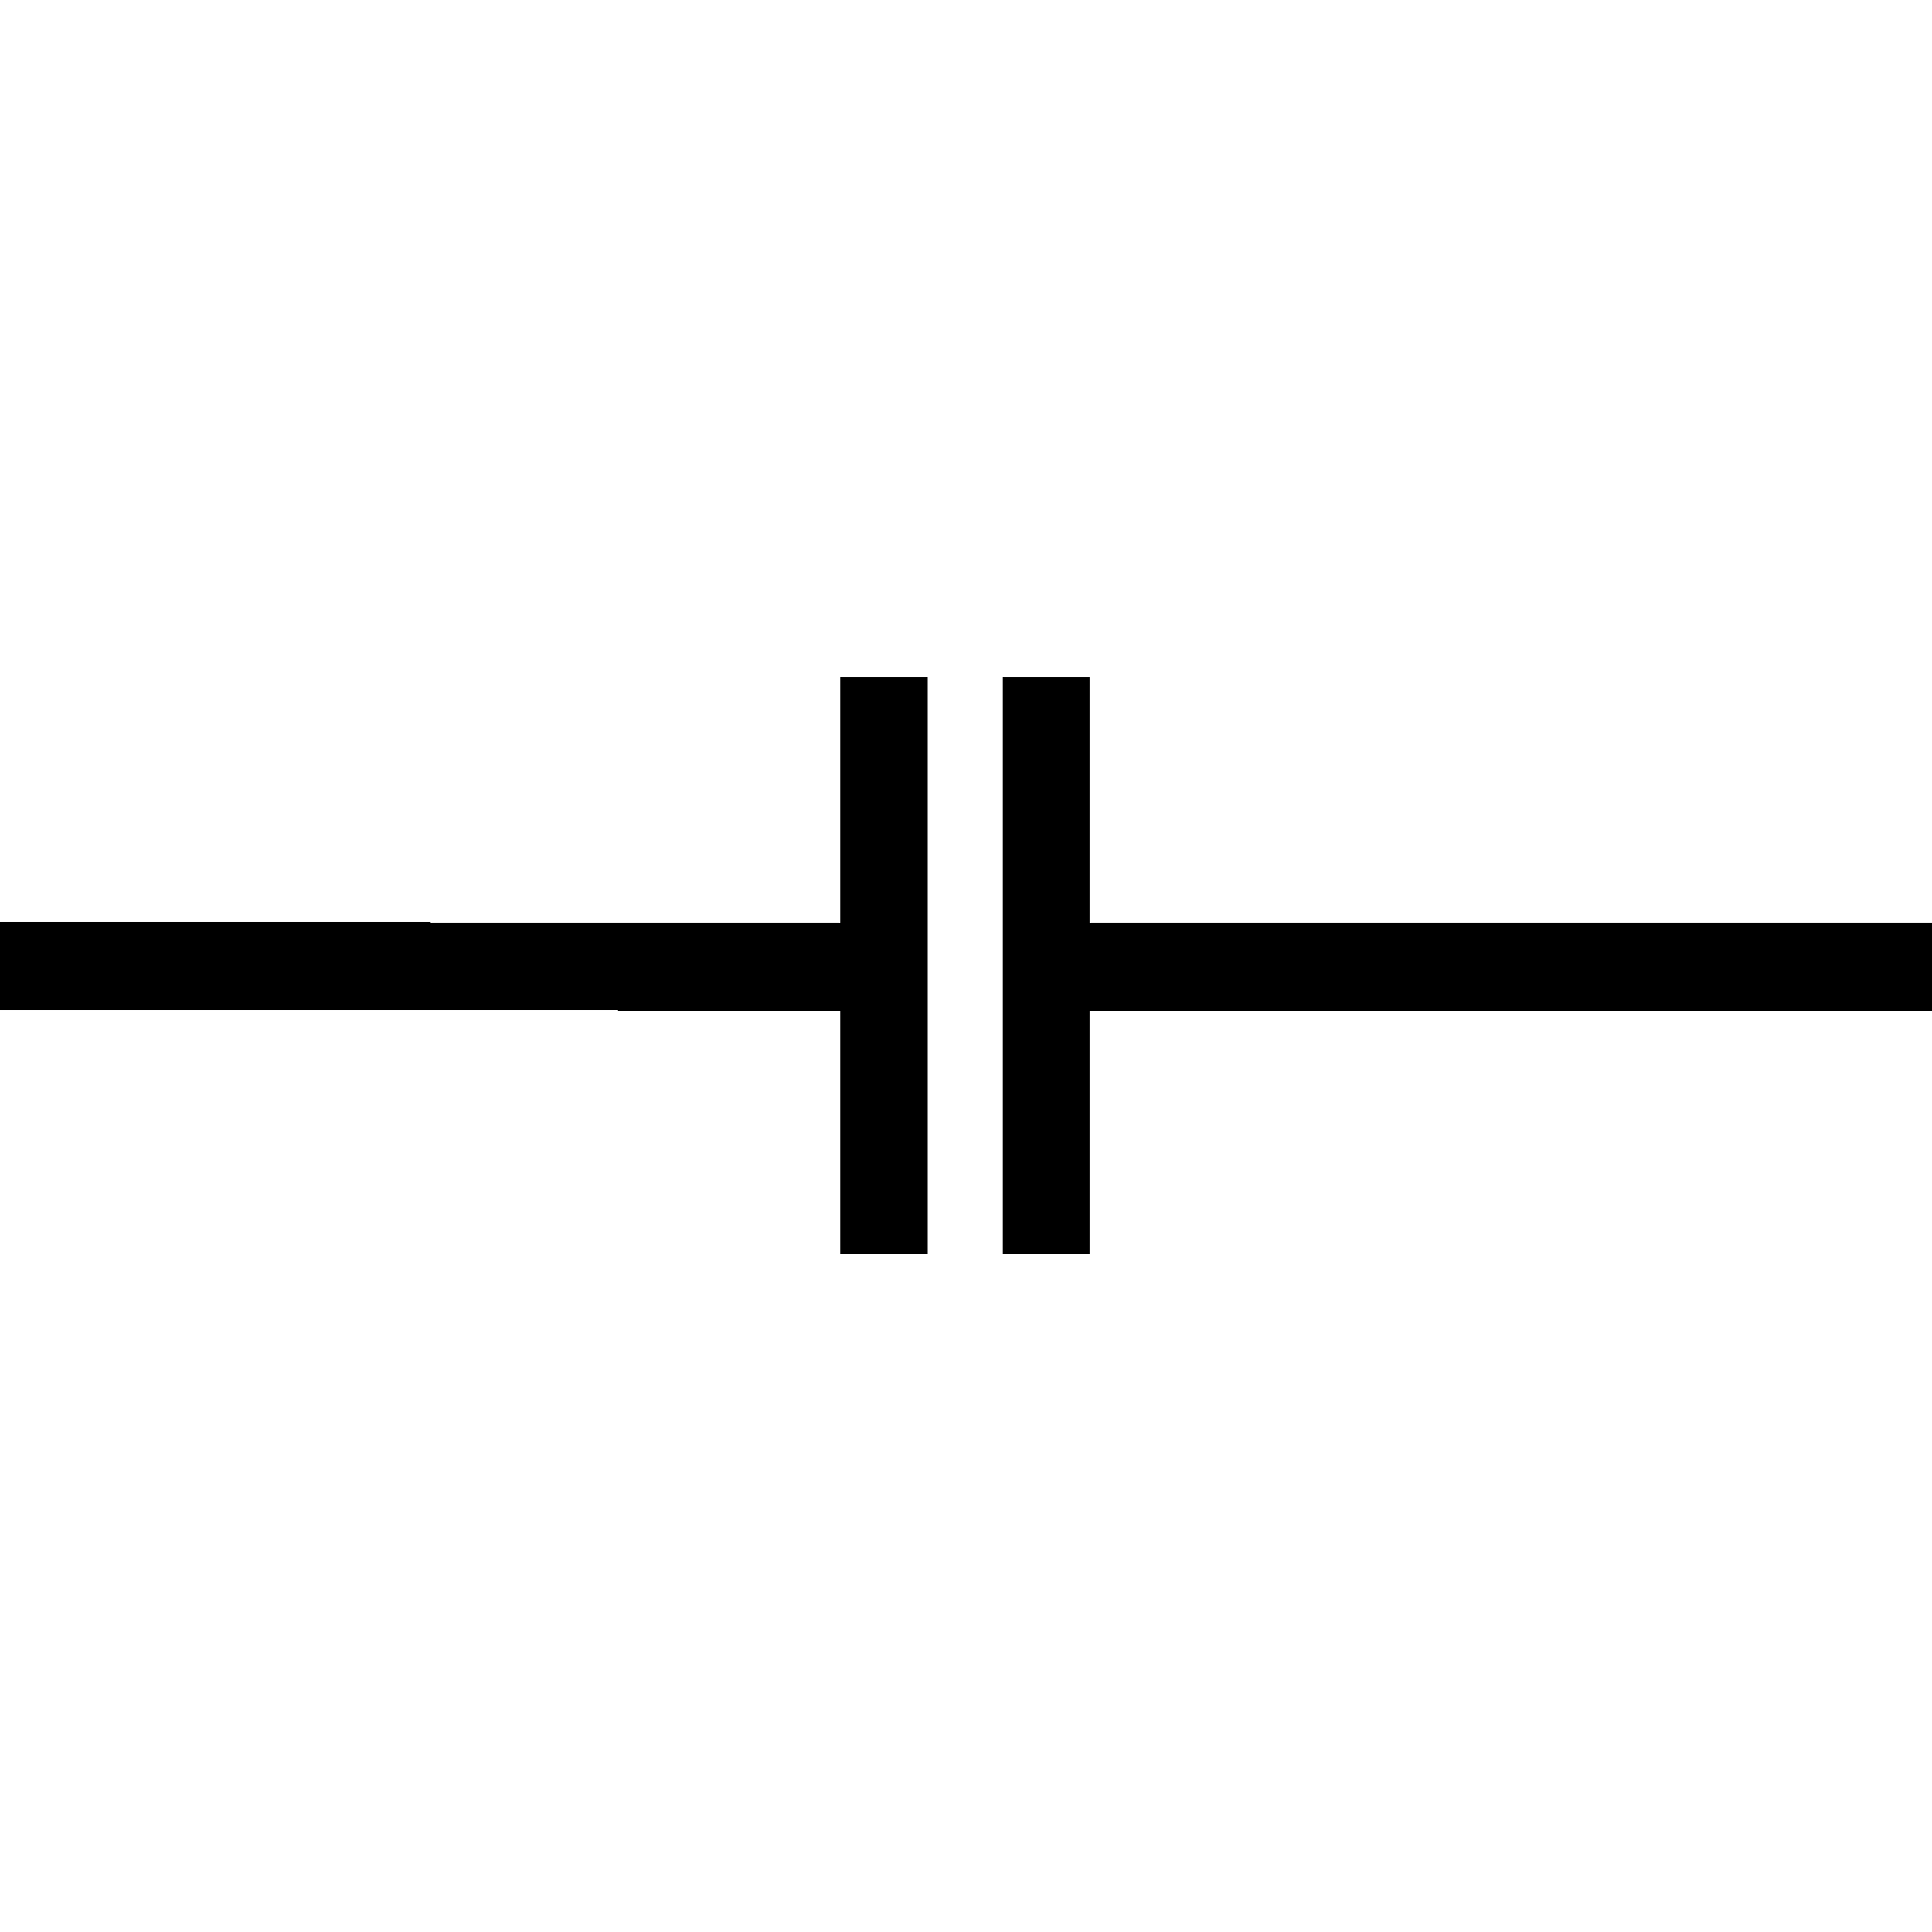
\includegraphics[width=0.15\linewidth]{images/5_memory/condensatore.pdf}
				\caption{Condensatore} 
		\end{figure}
	\end{columns}
\end{frame}


\begin{frame}
	\frametitle{La DRAM: dynamic RAM, }
	 
	\begin{figure}[!htbp] 
		\centering
		%\advance\leftskip-0.25cm
		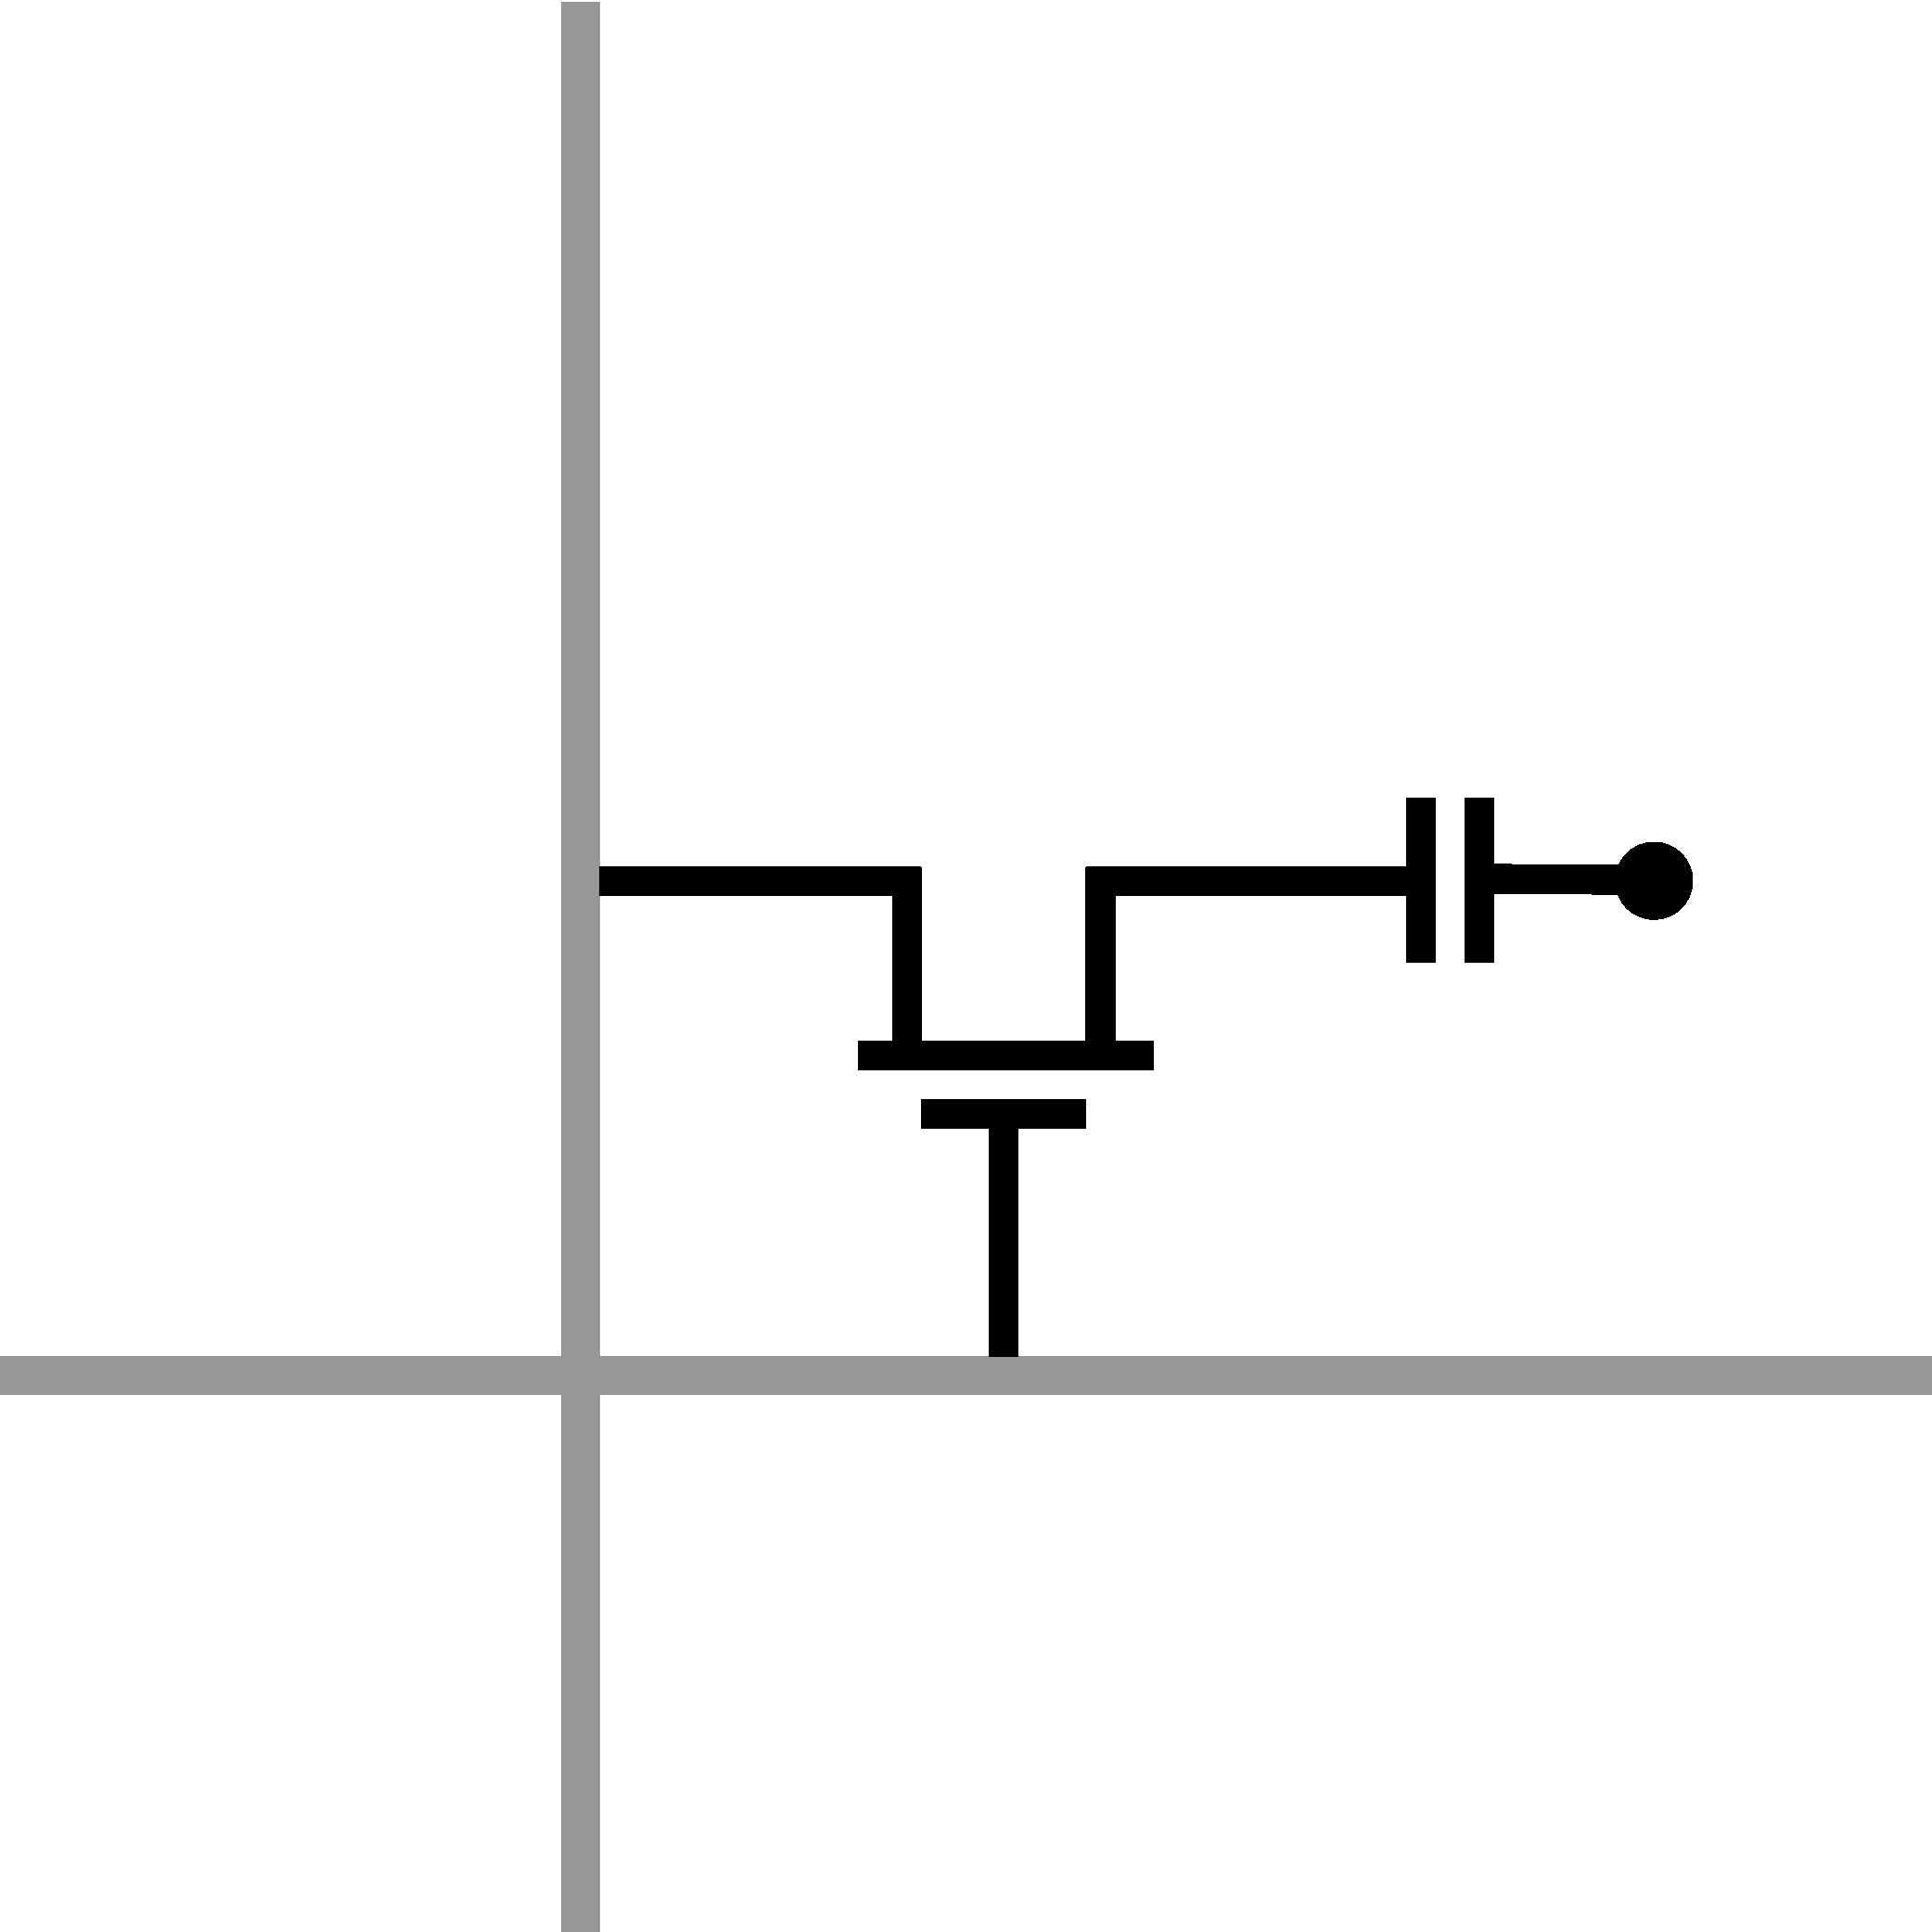
\includegraphics[width=0.6\linewidth]{images/5_memory/dram_bit.pdf}
		%\caption{PROM: nota la finestrella posta nella parte superiore del  circuito, che permette di ricevere i raggi UV}
	\end{figure}
	
\end{frame}


\begin{frame}
	\frametitle{La DRAM: dynamic RAM}
	 
	\begin{figure}[!htbp] 
		\centering
		%\advance\leftskip-0.25cm
		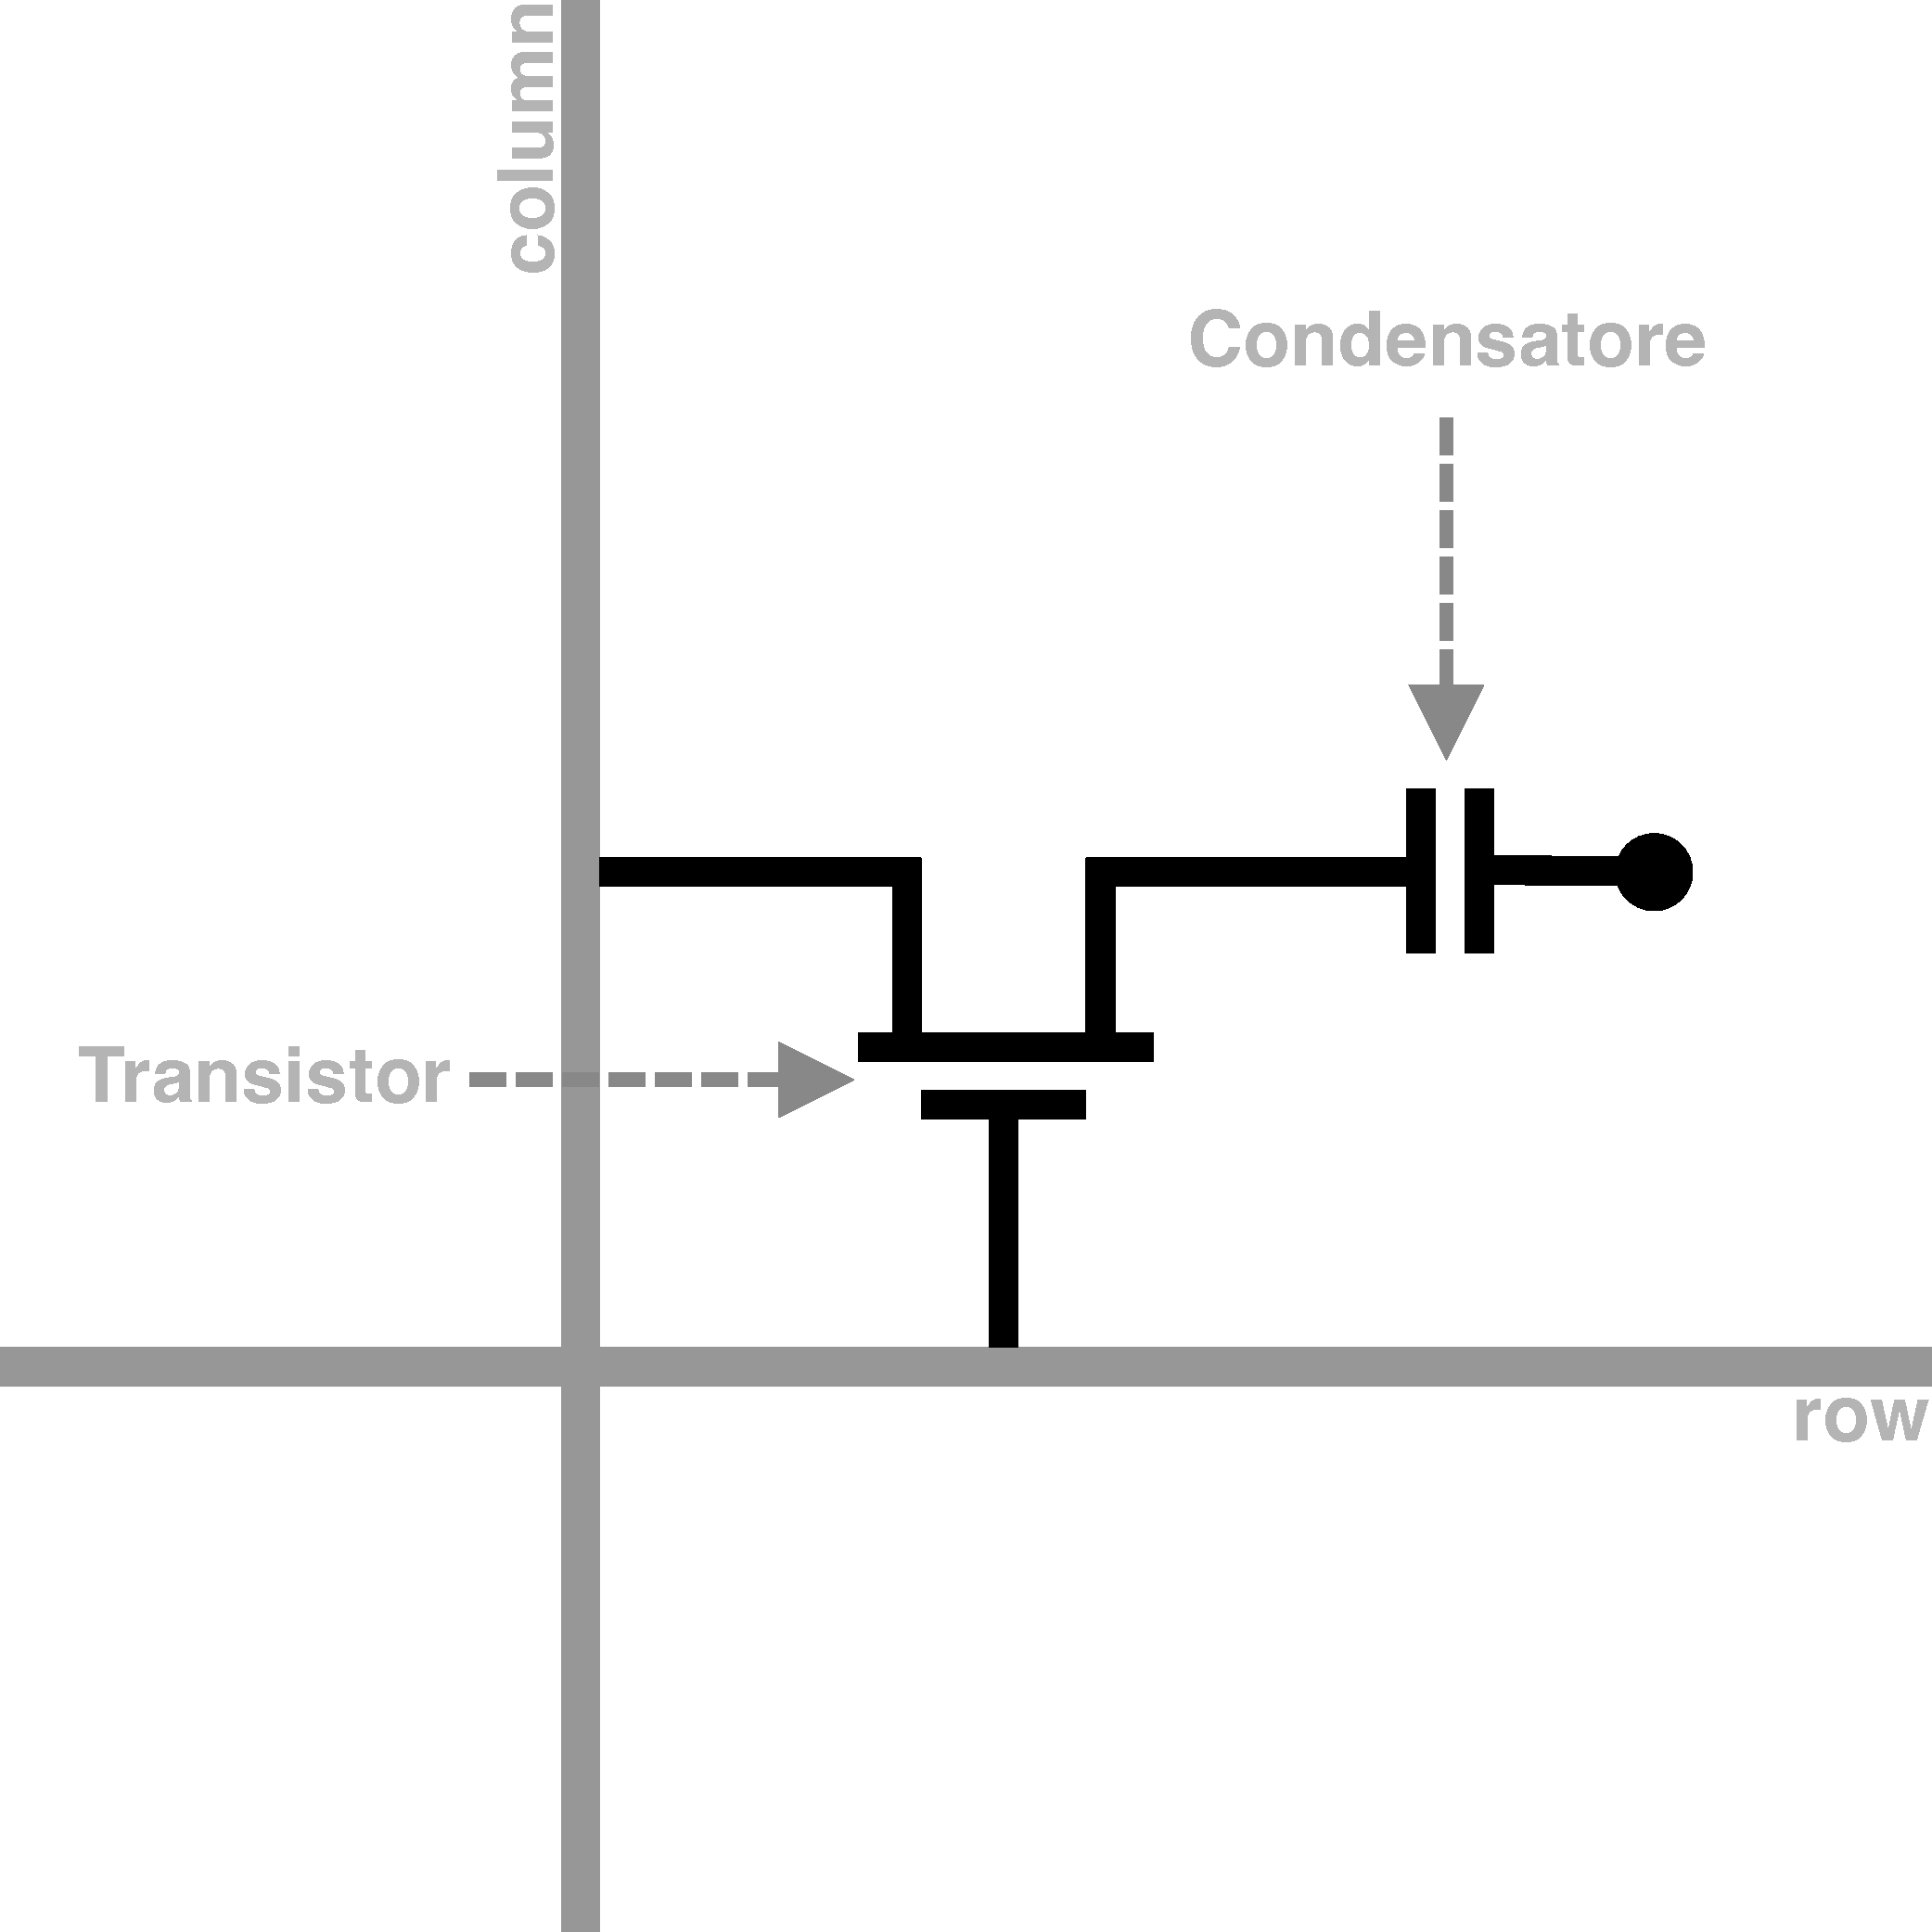
\includegraphics[width=0.6\linewidth]{images/5_memory/dram_bit_details.pdf}
		%\caption{PROM: nota la finestrella posta nella parte superiore del  circuito, che permette di ricevere i raggi UV}
	\end{figure}
	
\end{frame}


\begin{frame}
	\frametitle{La DRAM: dynamic RAM}
	 
	\begin{figure}[!htbp] 
		\centering
		%\advance\leftskip-0.25cm
		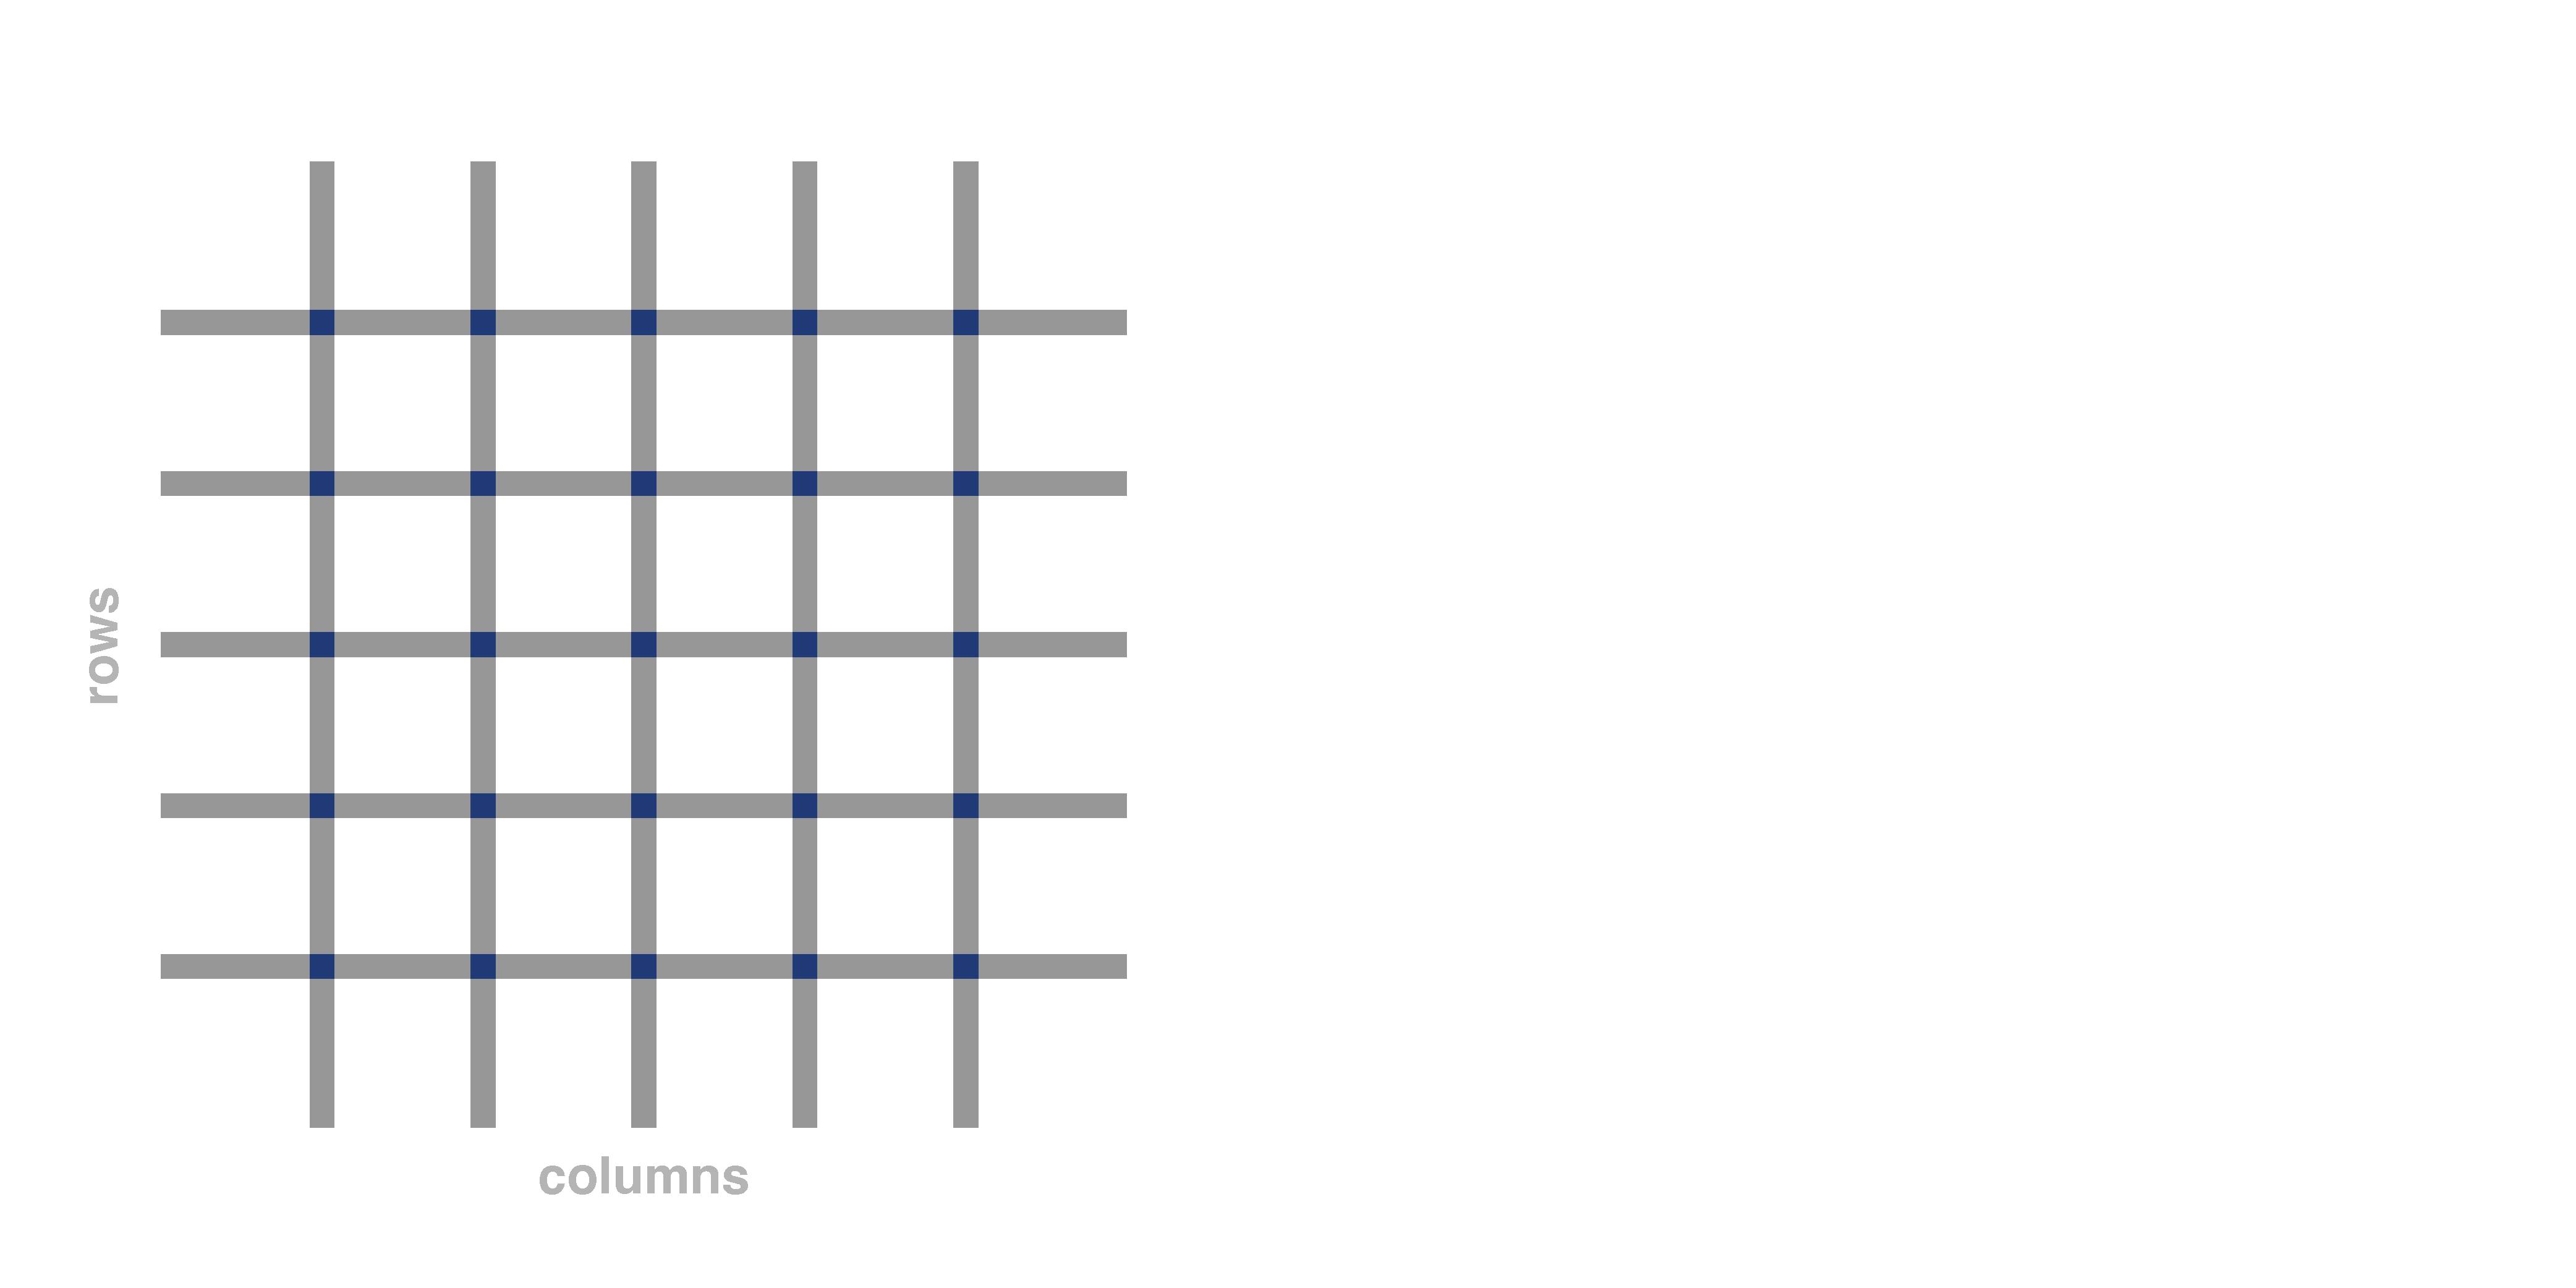
\includegraphics[width=1.0\linewidth]{images/5_memory/dram_matrix_1.pdf}
		%\caption{PROM: nota la finestrella posta nella parte superiore del  circuito, che permette di ricevere i raggi UV}
	\end{figure}
	
\end{frame}

\begin{frame}
	\frametitle{La DRAM: dynamic RAM}
	 
	\begin{figure}[!htbp] 
		\centering
		%\advance\leftskip-0.25cm
		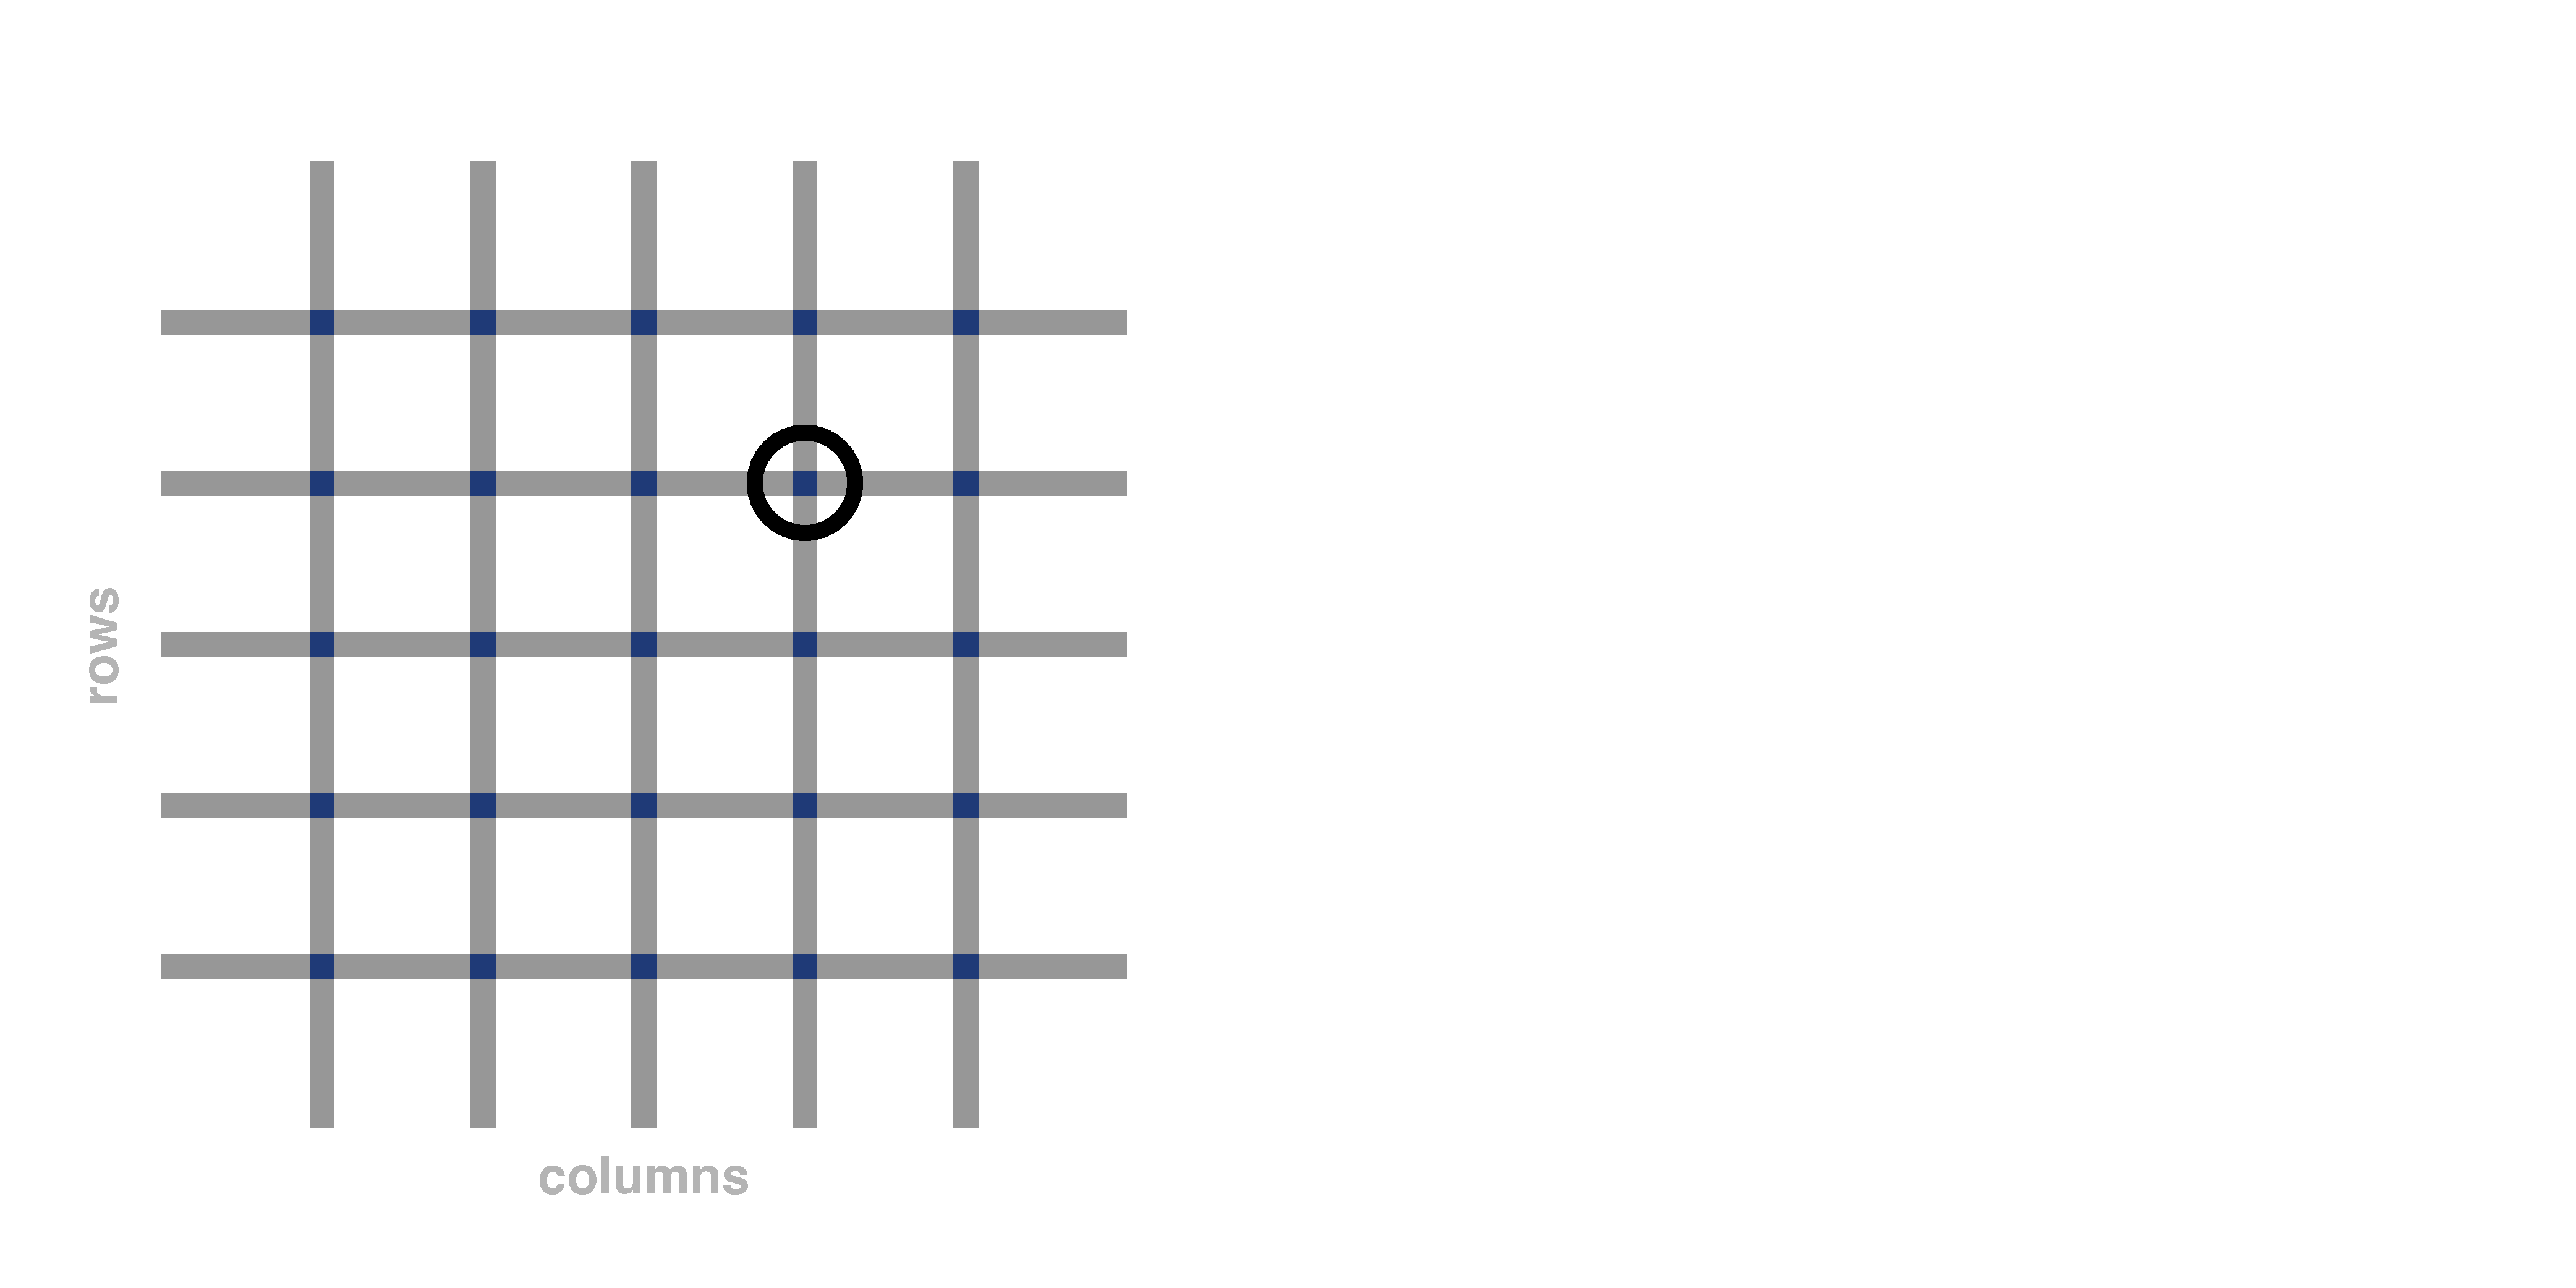
\includegraphics[width=1.0\linewidth]{images/5_memory/dram_matrix_2.pdf}
		%\caption{PROM: nota la finestrella posta nella parte superiore del  circuito, che permette di ricevere i raggi UV}
	\end{figure}
	
\end{frame}

\begin{frame}
	\frametitle{La DRAM: dynamic RAM}
	 
	\begin{figure}[!htbp] 
		\centering
		%\advance\leftskip-0.25cm
		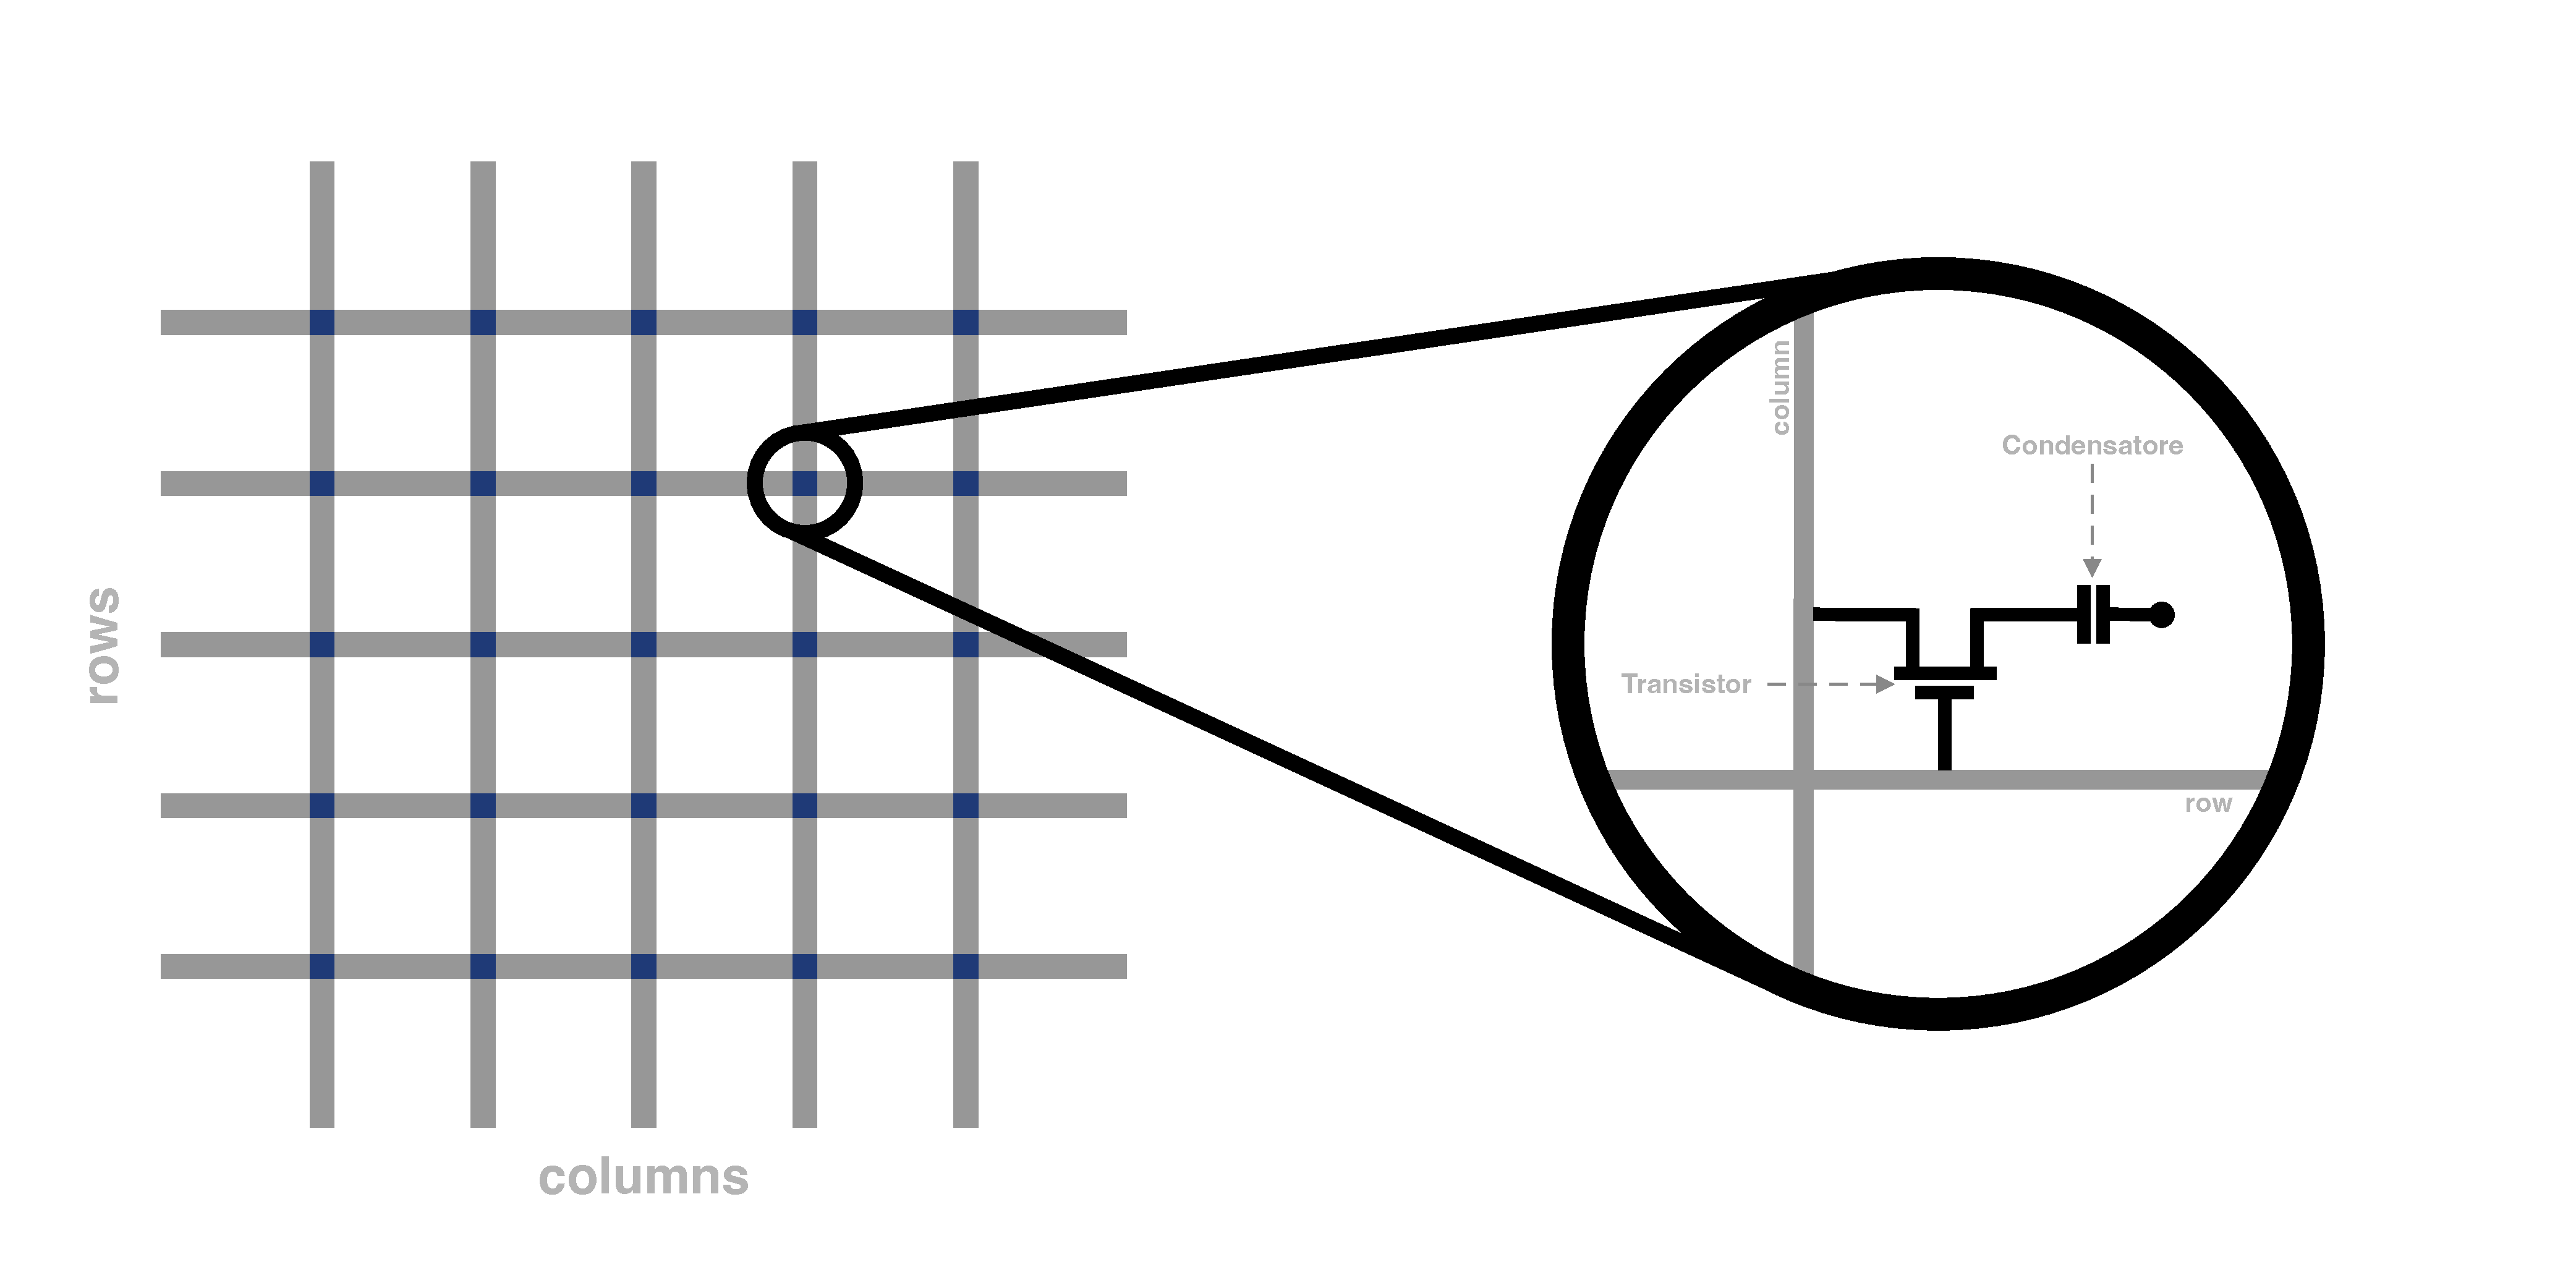
\includegraphics[width=1.0\linewidth]{images/5_memory/dram_matrix_3.pdf}
		%\caption{PROM: nota la finestrella posta nella parte superiore del  circuito, che permette di ricevere i raggi UV}
	\end{figure}
	
\end{frame}


\begin{frame}
	\frametitle{La DRAM: dynamic RAM}
	 
%	\begin{block}{Le prestazioni della memoria RAM}
%		Una delle strategie adottate per migliorare le prestazioni consiste nel combinare tipi di memoria veloce con tipi di memoria più capienti ma lente: un sistema gerarchico di memorie.
%	\end{block}
	
	\begin{figure}[!htbp] 
		\centering
		%\advance\leftskip-0.25cm
		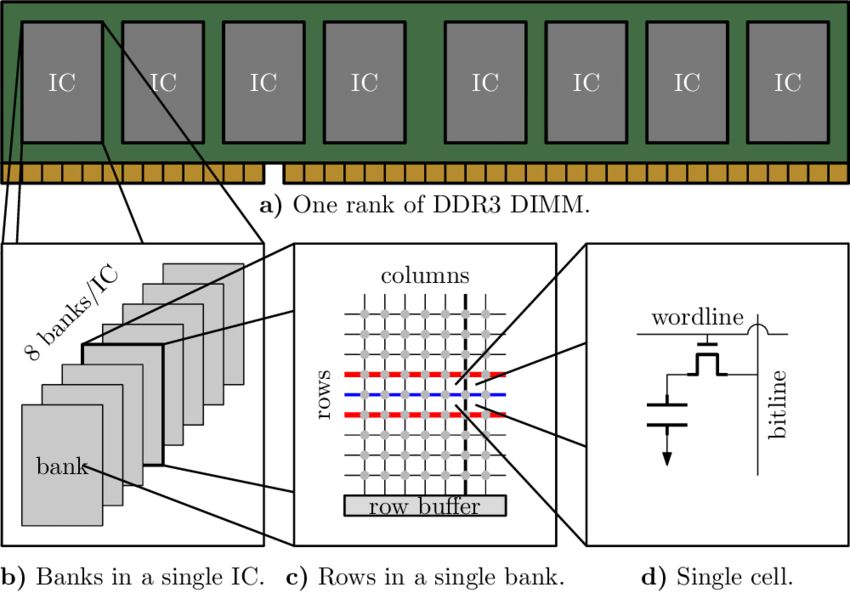
\includegraphics[width=0.8\linewidth]{images/5_memory/dram_organization.png}
%		\caption{La CPU: CU, ALU e registri}
		\label{fig:memory_dram_organization}
	\end{figure} 

\end{frame}


\begin{frame}
	\frametitle{La DRAM: dynamic RAM}
	
	\begin{columns}			
		\column{0.45\linewidth}
		\begin{scriptsize}
			\begin{figure}[!htbp]
				\centering
				\vspace{0.5em}
				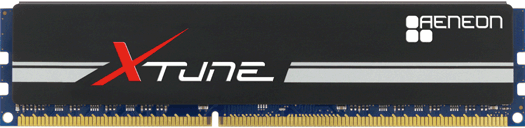
\includegraphics[width=0.9\linewidth]{images/5_memory/ddr3.png}
				\\DDR3 SDRAM - 240 pin - 5,25x1,18 inch\\\vspace{0.9em}
				
				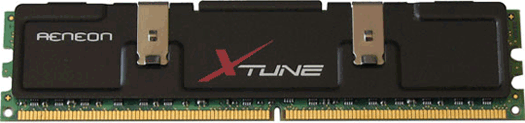
\includegraphics[width=0.9\linewidth]{images/5_memory/ddr2.png}
				\\DDR2 SDRAM - 240 pin - 5,25x1,18 inch\\\vspace{0.5em}
				
				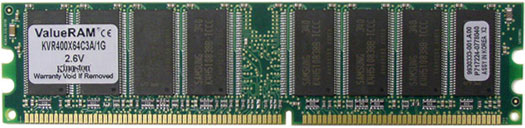
\includegraphics[width=0.9\linewidth]{images/5_memory/ddr1.png}
				\\DDR SDRAM - 184 pin - 5,375x1 inch\\\vspace{1em}
			\end{figure}
		\end{scriptsize}

		
		
		\column{0.55\linewidth}
		\begin{figure}[!htbp]
			\centering 
			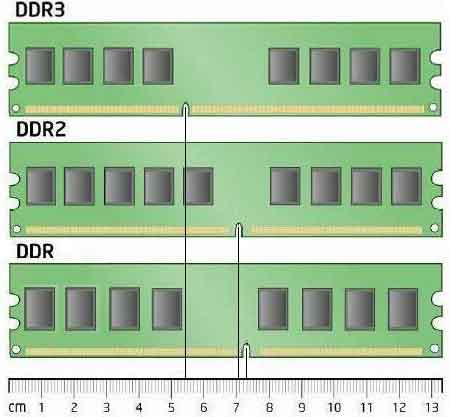
\includegraphics[width=1.0\linewidth]{images/5_memory/ddr_compare.png}
%			\caption{Confronto tra le diverse tipologie di DDR} 
		\end{figure}
	\end{columns}

\end{frame}


\begin{frame}
	\frametitle{La DRAM: dynamic RAM}
	 
	\begin{figure}[!htbp] 
		\centering
		%\advance\leftskip-0.25cm
		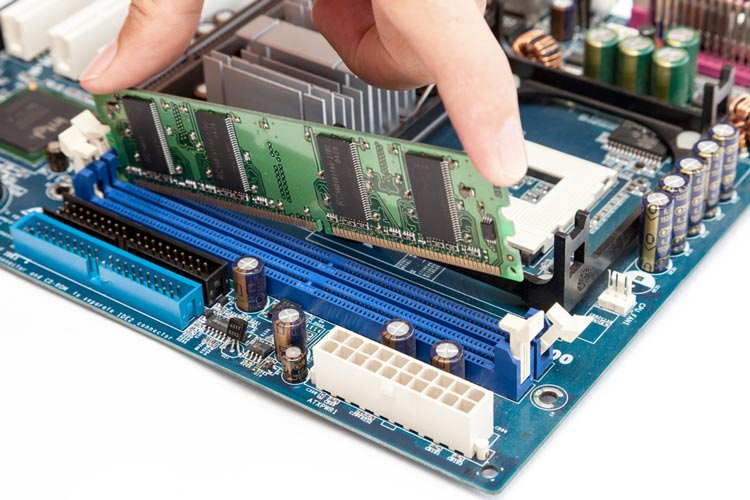
\includegraphics[width=0.9\linewidth]{images/5_memory/ram_installation.jpg}
		%\caption{}
	\end{figure}
	
\end{frame}


\begin{frame}
	\frametitle{La DRAM: dynamic RAM}
	 
%	La memoria RAM per PC viene realizzata in moduli:

	\begin{columns}			
		\column{0.5\linewidth}
		\begin{figure}[!htbp]
			\centering 
			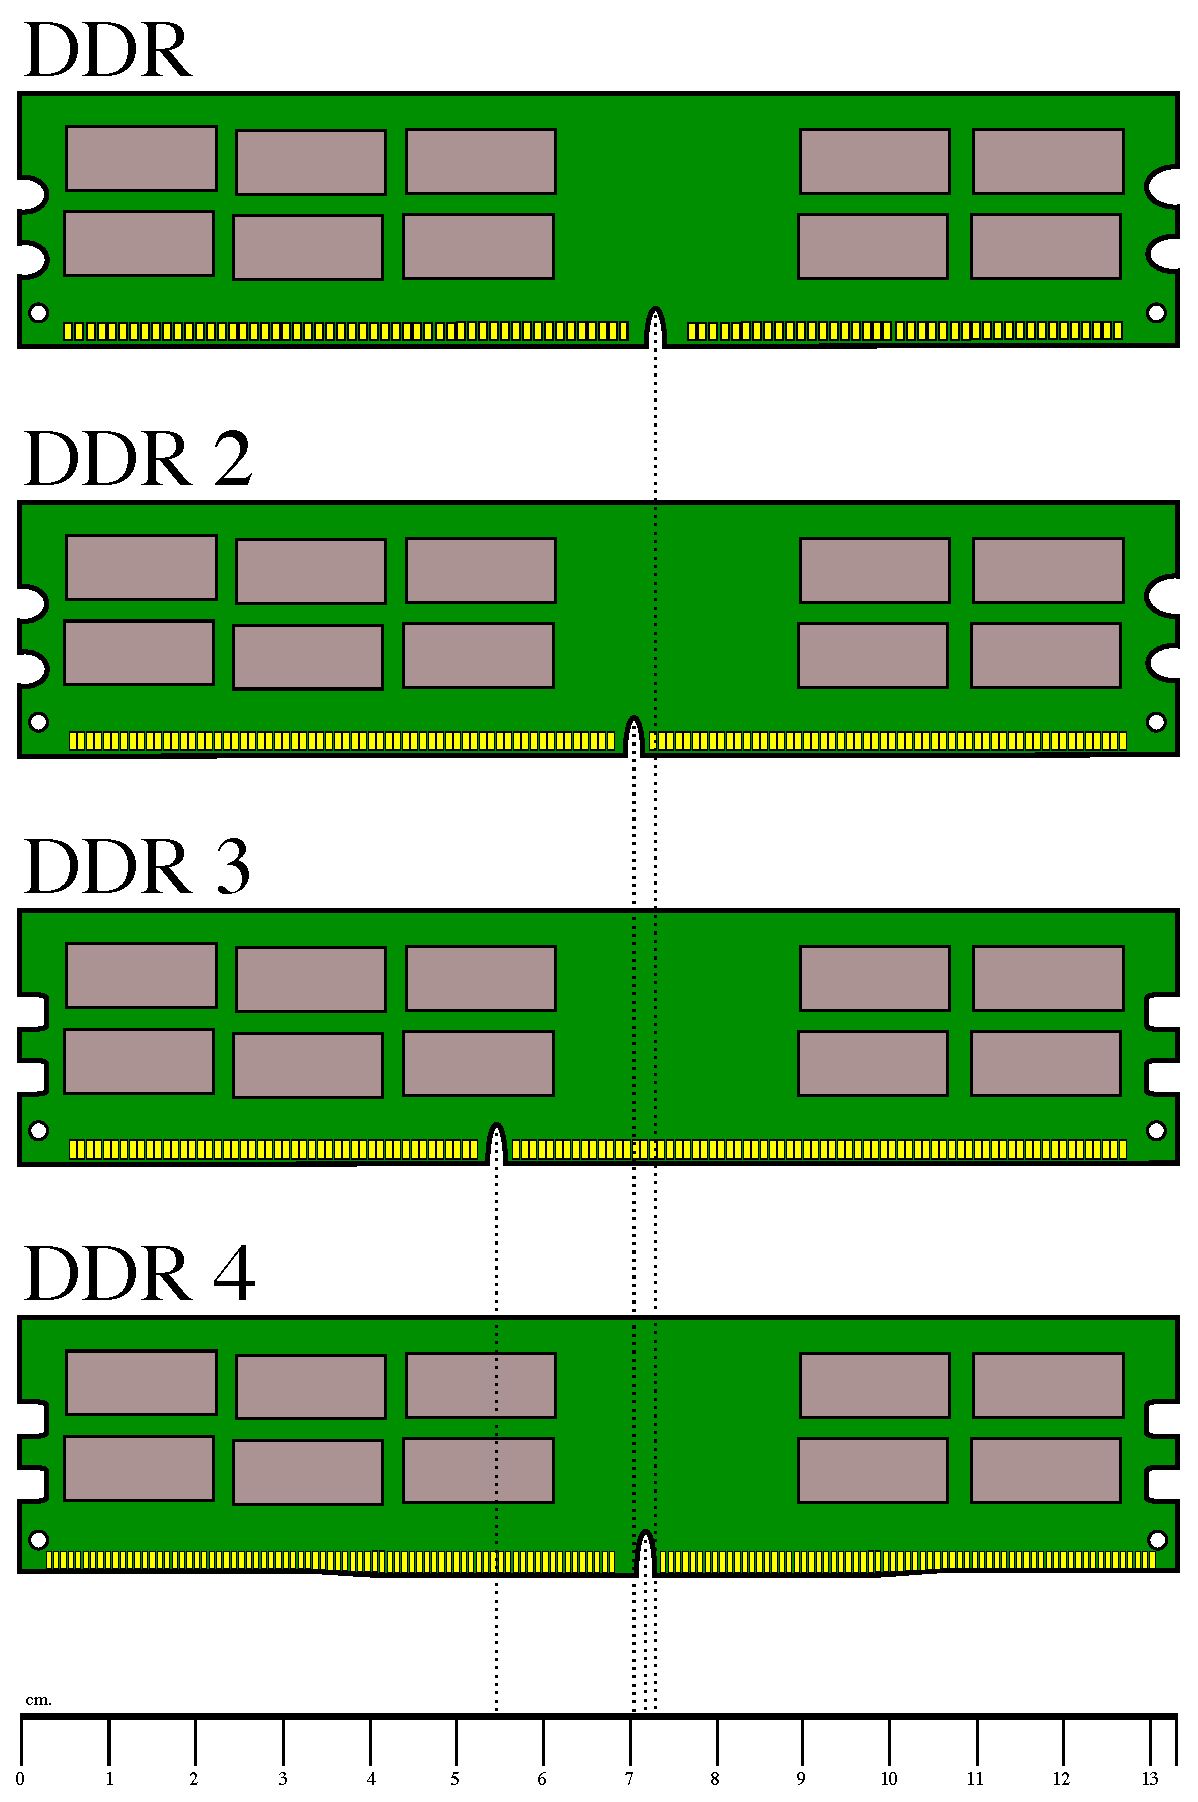
\includegraphics[width=0.63\linewidth]{images/5_memory/dimm.pdf}
			\caption{Per PC desktop: \protect\linebreak DIMM (Dual Inline Memory Module)}
			\label{fig:memory_dimm}
		\end{figure}

		\column{0.5\linewidth}
		\begin{figure}[!htbp]
			\centering 
			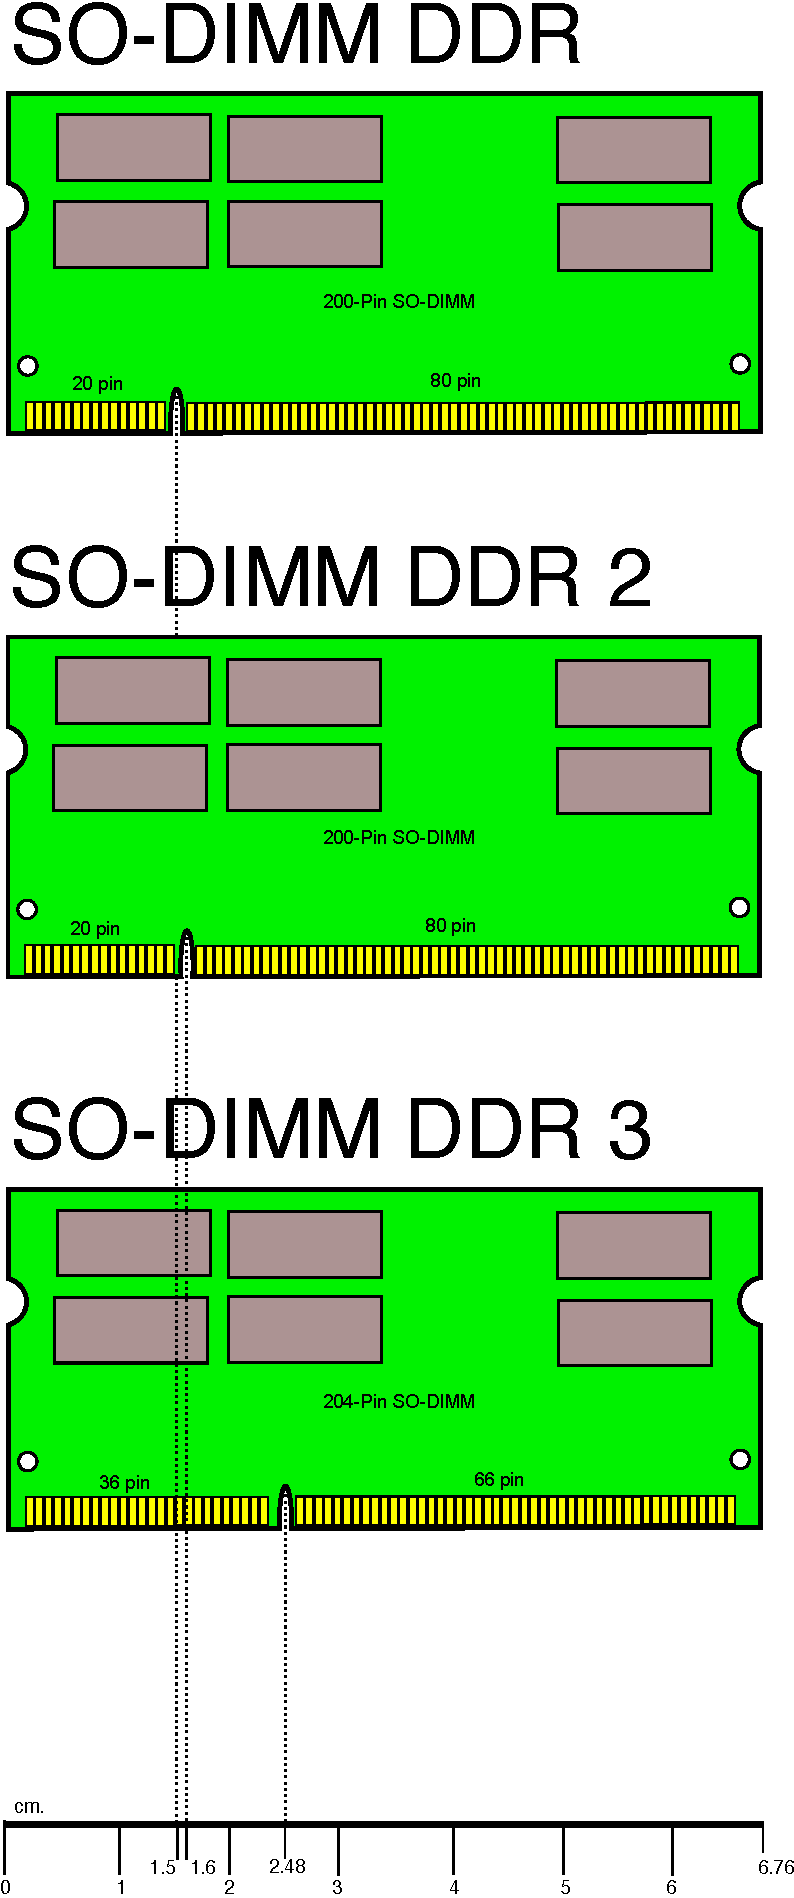
\includegraphics[width=0.4\linewidth]{images/5_memory/so_dimm.pdf}
			\caption{Per PC notebook: \protect\linebreak SO-DIMM (Small Outline DIMM)}
			\label{fig:memory_so_dimm}
		\end{figure}
	\end{columns}
	
\end{frame}




\begin{frame}
	\frametitle{La DRAM: dynamic RAM}
	 
	\begin{figure}[!htbp] 
		\centering
		%\advance\leftskip-0.25cm
		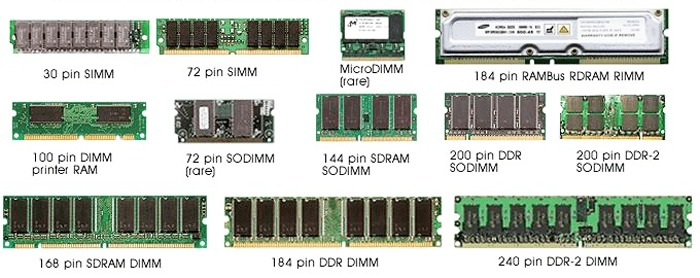
\includegraphics[width=1.0\linewidth]{images/5_memory/ram_types.jpeg}
		%\caption{}
	\end{figure}
	
\end{frame}






%\subsubsection[La SDRAM: synchronized dynamic RAM]{La SDRAM: synchronized dynamic RAM}
% https://www.nexthardware.com/forum/ram/41922-latenze-ram-parametri-e-descrizione-cura-di-swarzy.html
\begin{frame}
	\frametitle{La RAM: valutare le prestazioni di una RAM}
	
	\begin{block}{}
		La velocità di trasferimento è notevolmente influenzata dai fenomeni di latenza, che si verificano durante le operazioni di lettura/scrittura e che dipendono strettamente dal tipo e dalla qualità del chip, nonché dalla frequenza di funzionamento. Ad ogni banco di memoria vengono associati dei tempi caratteristici detti timing, misurati in unità di cicli di clock: a valori più bassi corrispondono prestazioni migliori, a parità di frequenza.\\~\\
		
		I timing più importanti sono (vedi \underline{\href{https://it.wikipedia.org/wiki/DDR\_SDRAM}{link}}):
		\begin{itemize}
			\item CAS Latency Time (tCl)
			\item RAS to CAS Delay Time (tRCD)
			\item RAS Precharge Time (tRP)
			\item Active-to-Precharge Delay (tRAS)
			\item Row Cycle Time (tRC)
		\end{itemize}
		
	\end{block}

	
	
\end{frame}


\subsubsection[La SRAM: static RAM]{La SRAM: static RAM}
\begin{frame}
	\frametitle{La SRAM: static RAM}
	  
	\begin{block}{}
		Le \textbf{SRAM}, acronimo di static RAM, sono sempre memorie volatili ma non necessitano di refresh. I flip-flop sono alla base della memorizzazione di un singolo bit in queste tipologie di memoria.\\~\\
		I banchi di SRAM consentono di mantenere le informazioni per un tempo teoricamente infinito, hanno \textbf{bassi tempi di lettura} e \textbf{bassi consumi}. La necessità di usare molti componenti per cella le rende però \textbf{più costose} delle DRAM.\\~\\
		Sono solitamente usate per le memorie cache, dove elevate velocità e ridotti consumi sono caratteristiche fondamentali. Ad esempio, possono essere trovate nella cache L1, L2 o L3 di un processore.
		
	\end{block}
\end{frame}


% https://superuser.com/questions/196143/where-exactly-l1-l2-and-l3-caches-located-in-computer
\begin{frame}
	\frametitle{La DRAM: dynamic RAM}
	 
	\begin{figure}[!htbp] 
		\centering
		%\advance\leftskip-0.25cm
		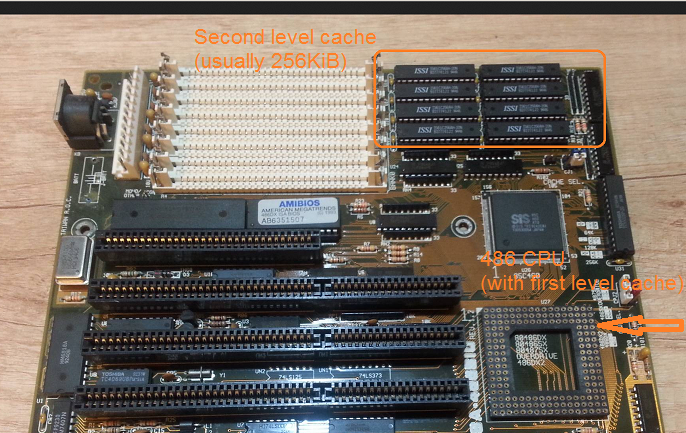
\includegraphics[width=0.62\linewidth]{images/5_memory/cache_1.png}
		\caption{\textbf{80486 (1989):} questa è la prima CPU di questa generazione che ha un po' di cache sulla CPU. È una cache unificata da 8 KB, il che significa che viene utilizzata per dati e istruzioni. In questo periodo diventa comune inserire 256 KB di memoria statica veloce sulla scheda madre come cache di 2° livello. Quindi cache di 1° livello sulla CPU, cache di 2° livello sulla scheda madre.}
	\end{figure}
	
\end{frame}


\begin{frame}
	\frametitle{La DRAM: dynamic RAM}
	 
	\begin{figure}[!htbp] 
		\centering
		%\advance\leftskip-0.25cm
		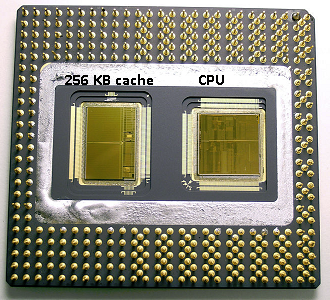
\includegraphics[width=0.42\linewidth]{images/5_memory/cache_2.png}
		\caption{\textbf{\href{https://en.wikipedia.org/wiki/Pentium\_Pro}{Pentium Pro '80686'} (1995):} a seconda del modello, questo chip aveva una cache integrata da 256Kb, 512KB o 1MB. Si noti che metà dello spazio nel chip è utilizzato dalla cache. E questo è per il modello da 256KB. Il prezzo di mercato era piuttosto alto per l'epoca. Si noti inoltre che questo chip contiene due matrici. Uno con la CPU e la prima cache, l'altro con la seconda cache da 256 KB.}
	\end{figure}
	
\end{frame}


\begin{frame}
	\frametitle{La DRAM: dynamic RAM}
	 
	\begin{figure}[!htbp] 
		\centering
		%\advance\leftskip-0.25cm
		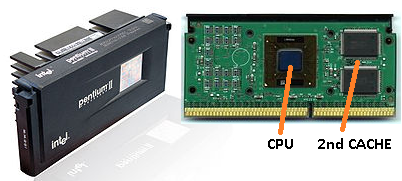
\includegraphics[width=0.8\linewidth]{images/5_memory/cache_3.png}
		\caption{\textbf{\href{https://en.wikipedia.org/wiki/Pentium\_Pro}{Pentium-2}:} per ragioni economiche la seconda cache viene spostata fuori dalla CPU. Solo successivamente, man mano che la tecnologia è avanzata, diventò più accessibile dal punto di vista dei costi rimettere la seconda cache all'interno della CPU.}
	\end{figure}
	
\end{frame}



\begin{frame}
	\frametitle{La DRAM: dynamic RAM}
	 
	\begin{figure}[!htbp] 
		\centering
		%\advance\leftskip-0.25cm
		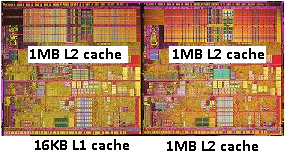
\includegraphics[width=0.8\linewidth]{images/5_memory/cache_4.png}
		\caption{\textbf{Pentium-D (duo):} che fondamentalmente corrispondono a due core pentium-4 sullo stesso chip. La cache di secondo livello viene condivisa tra i due core, una cache di secondo livello condivisa è globalmente più veloce di avere due cache di secondo livello indipendenti di dimensioni dimezzate.}
	\end{figure}
	
\end{frame}


\begin{frame}
	\frametitle{La DRAM: dynamic RAM}
	 
	\begin{figure}[!htbp] 
		\centering
		%\advance\leftskip-0.25cm
		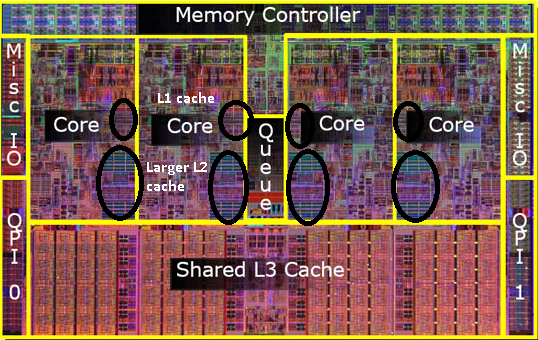
\includegraphics[width=0.8\linewidth]{images/5_memory/cache_5.png}
		\caption{\textbf{Processore i7:} più cores, stesso ragionamento, usando una cache di terzo livello condivisa tra i core.}
	\end{figure}
	
\end{frame}





